\documentclass[12pt,a4paper,titlepage,listof=totoc,bibliography=totoc,chapteratlists=0pt]{scrreprt}
\input{global-const.tex}
\input{header}

\def\thesislang{en}

\makeatletter
\def\bstctlcite{\@ifnextchar[{\@bstctlcite}{\@bstctlcite[@auxout]}}
\def\@bstctlcite[#1]#2{\@bsphack
	\@for\@citeb:=#2\do{%
		\edef\@citeb{\expandafter\@firstofone\@citeb}%
		\if@filesw\immediate\write\csname #1\endcsname{\string\citation{\@citeb}}\fi}%
	\@esphack}
\makeatother

\clubpenalty=10000 
\widowpenalty=10000
\displaywidowpenalty=10000
\interfootnotelinepenalty=10000

\title{\thesistitle}
\makeatletter
\@ifundefined{fourthauthor}{
  \@ifundefined{thirdauthor}{
    \author{\firstauthor, \secondauthor}
  }{
    \author{\firstauthor, \secondauthor, \thirdauthor}
  }
}{
  \author{\firstauthor, \secondauthor, \thirdauthor, \fourthauthor}
}
\makeatother

\makeindex
\makeglossaries
\newacronym{trp}{TRP}{TestRail Procedure}
\newacronym{ebnf}{EBNF}{Extended Backus–Naur form}

% Usage:
% \gls{label} lowercase in text
% \Gls{label} Uppercase in text
% \newacronym{label}{abbrev}{full}
% \newglossaryentry{label}{settings}



\begin{document}
\bstctlcite{IEEEexample:BSTcontrol}
\newcommand{\reminder}[1]
{ \textcolor{red}{<[{\bf\marginpar{\mbox{$<==$}} #1 }]>} }
\newcommand{\icode}[1]{\lstinline$#1$}
%\urlstyle{same}
%\setstretch{1.5}
\setstretch {1.433}
\renewcommand{\arraystretch}{1.2}

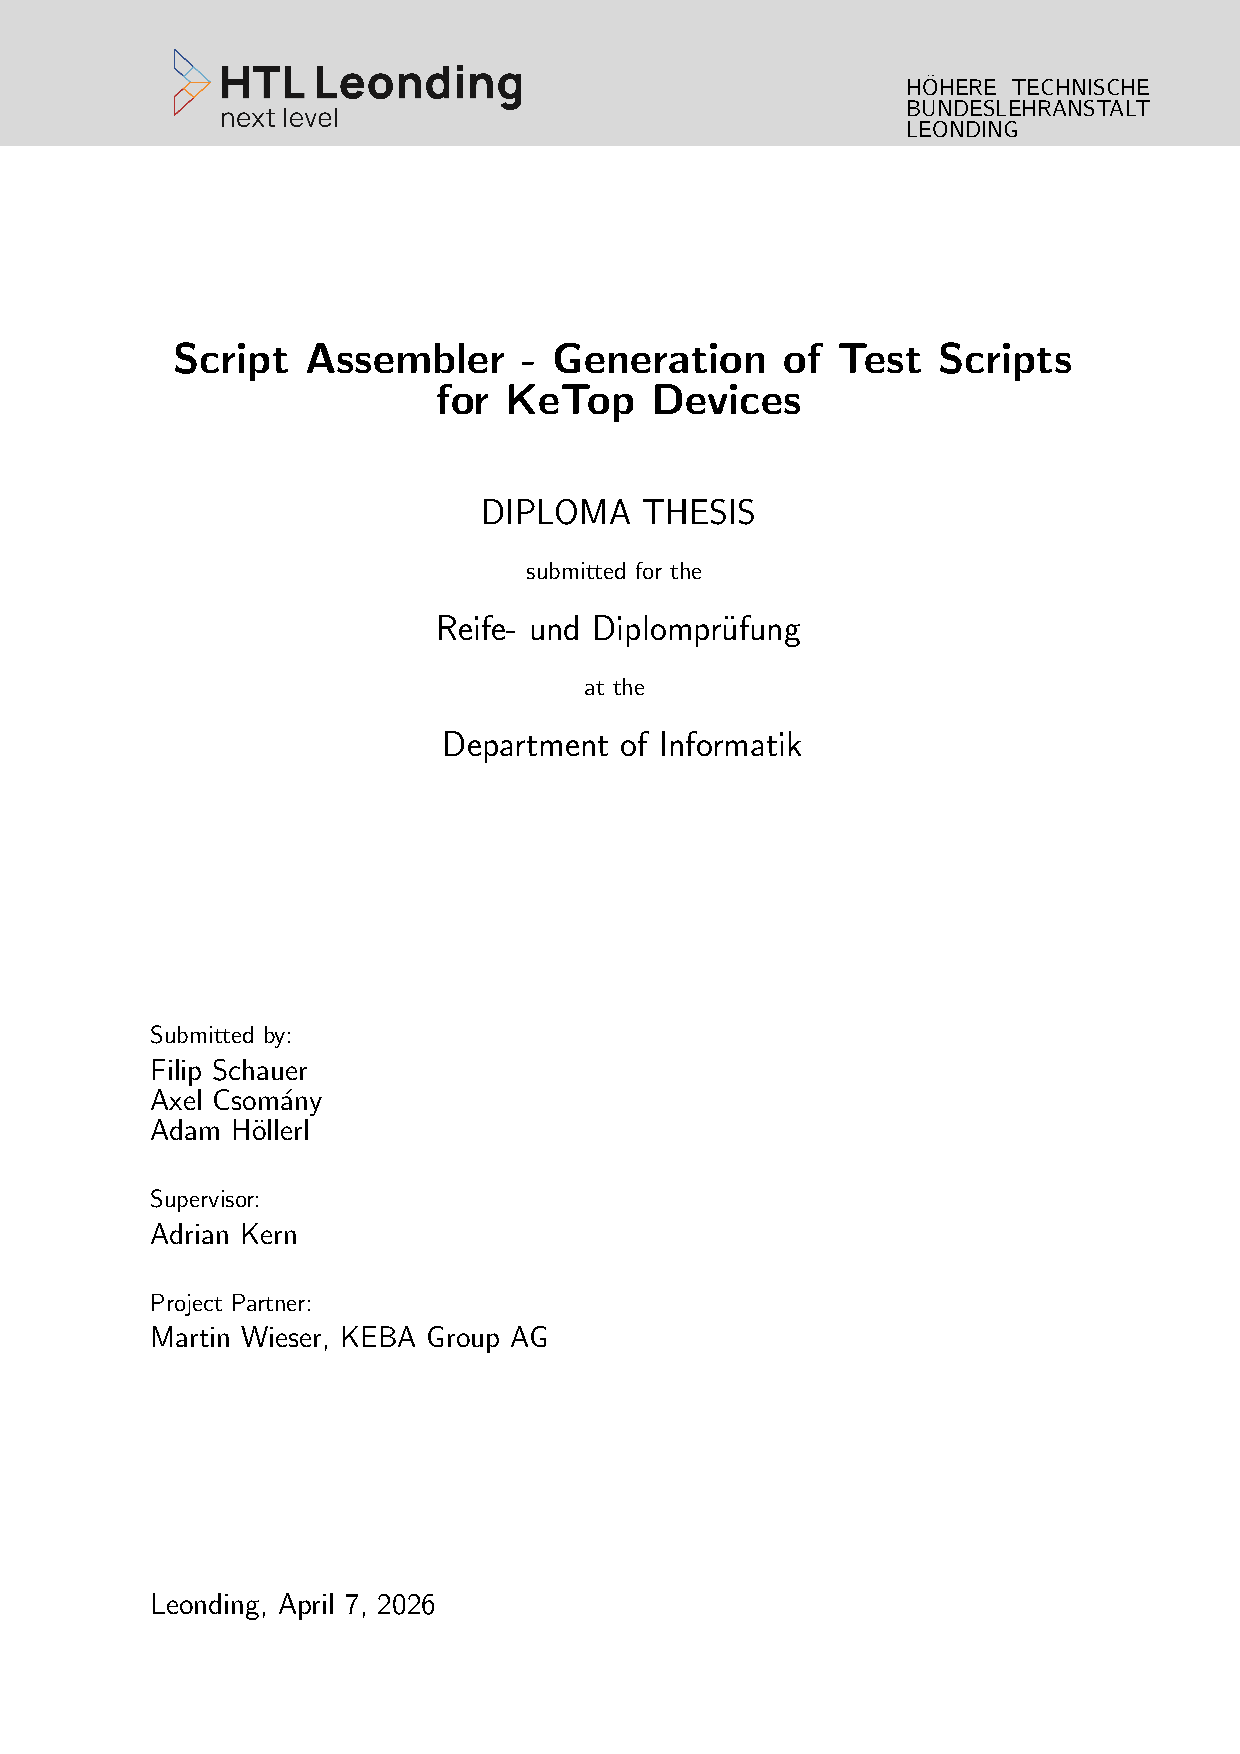
\includepdf{./titlepage/coversheet}
\pagenumbering{Roman}
\newpage
\input{oath}
\begin{spacing}{1}
    \chapter*{Abstract}
\end{spacing}

This thesis presents and documents new features and improvements to the internal testing system of the KEBA Group AG, an Austrian technology company specializing in automation systems for industry, banking and energy applications. 

After analyzing the initial problems and how to solve them, various used technologies and concepts are explained. This includes generally known systems such as Python and PostgreSQL, as well as more specific concepts such as the Robot Framework and the Monaco Editor.

Next, the thought process and implementation of the new features and improvements is described in detail. The new functionalities include the creation of a new EBNF-based test script format, the definiton of a new set of keywords for the test scripts and the development of a new alternative database system for the test data. 



\newpage
\begin{spacing}{1}
    \chapter*{Zusammenfassung}
\end{spacing}

Diese Diplomarbeit präsentiert und dokumentiert neue Funktionen und Verbesserungen am internen Testsystem der KEBA Group AG, einem österreichischen Technologieunternehmen, das sich auf Automatisierungssysteme für Industrie, Banken und Energieanwendungen spezialisiert.

Nach der Analyse der anfänglichen Probleme und deren möglichen Lösungen werden verschiedene verwendete Technologien und Konzepte erklärt. Dazu gehören allgemein bekannte Systeme wie Python und PostgreSQL sowie spezifischere Konzepte wie das Robot Framework und der Monaco Editor.

Anschließend wird der Denkprozess und die Implementierung der neuen Funktionen und Verbesserungen im Detail beschrieben. Zu den neuen Funktionalitäten gehören die Erstellung eines neuen EBNF-basierten Testskriptformats, die Definition von neuen Schlüsselwörtern für die Testskripte und die Entwicklung eines neuen alternativen Datenbanksystems für die Testdaten.

\chapter*{Acknowledgements}

The team behind this diploma thesis would like to wholeheartedly thank Martin Wieser and Martin Fuchs for their continuious guidance and support throughout the making of this project.

Furthermore, we especially thank Adrian Kern for his essential guidance and his patience.

\section*{Filip Schauer's Acknowledgements}

Without my parents and my sister by my side, I probably would have given up by now. I would like to thank them for their consistent support throughout my education, my internships, and this thesis. 

\section*{Axel Csomány's Acknowledgements}

I want to give huge thanks to my friends and family, that have always been supporting me.

My most special thanks is dedicated to my mother. It is thanks to her that I made it this far. May you rest in peace.

\section*{Adam Höllerl's Acknowledgements}

I would like to thank my family for their constant support, encouragment

\pagestyle{plain}

\IfStrEq{\thesislang}{de}
{
	\renewcommand{\lstlistlistingname}{Quellcodeverzeichnis}
}
{
 % keep at list of listing
}
% Set English listing, figures and tables names when thesislang is 'en'
\IfStrEq{\thesislang}{en}{
	\renewcommand{\lstlistlistingname}{List of Listings}
	\renewcommand{\listfigurename}{List of Figures}
	\renewcommand{\listtablename}{List of Tables}
}{}
\tableofcontents
\newpage
\setcounter{RPages}{\value{page}}
\setcounter{page}{0}
\pagenumbering{arabic}
\pagestyle{scrheadings}

% ==========================================
% PART I: INTRODUCTION
% ==========================================
\part{Introduction [X, F]}\label{part:introduction}

\chapter{Background [X]}\label{chap:background}
\setauthor{Axel Csomány}
\section{KEBA Group AG}

For more than 50 years the technology company KEBA Group AG has been providing various customers with solutions to their unique problems. Among its three main branches, the Industrial Automation branch focuses primarily on the needs of the individual situation as the hardware and its software get built.

The company was founded 1968 in Linz, Austria. Today with 28 establishments in 16 different countries and more than 2000 employees they are internationally active.

\chapter{Initial Problem [X]}\label{chap:problem}
\setauthor{Axel Csomány}
\section{Current Testing Strategy and its Flaws}

So called "KeTops" are used as operating devices to control machines of varying structure and complexity. These machines and their corresponding KeTops differ in their configuration from each customer which is why fitting test scripts are required. These test scripts examine all aspects of the device from the installed operating system to software specific behaviors. 

The \textit{Script Assembler} which is used in current production is able to merge a number of test scripts together for this use. The hard-coded nature and resulting limited maintainibility of the Script Assembler is its primary flaw. Furthermore all data concerning tests are saved and maintained in a TestRail database which although functional, heavily limits the expandability and independence of the testing environment.

\section{Acceptance Tests}

The Robot Framework is a test automation framework designed to create and execute the test scripts in the current system. These tests are acceptance tests, which are a type of test that is created before the actual implementation of the software. The purpose of acceptance tests is to define the expected behavior of the system from the perspective of the customer or end-user. They serve as a guide to ensure that the development team is building the software according to the expectations of said customer \cite{WikiRobotFramework}.

Acceptance tests typically consist of terms understandable by both technical and non-technical parties, making them understandable regardless of the expertise of the reader. They intend to cover all the requirements and functionalities of the system and serve as a list of criteria for acceptance \cite{WikiAcceptanceTestDrivenDev}.

\subsection{Different Types of Tests and the V-Model}

The V-Model emphasizes the importance of consistent testing throughout the development process of software. In the first half of the V-Model, the focus is on defining the concept of the system as a whole and its requirements. Further on, the definition is broken down into smaller and smaller components, until we reach the detailed design of the software. Afterwards, the implementation takes place, which is the point where the actual code is written.

The second half of the V-Model focuses on testing each corresponding unit on the same level of the first half. During each design phase, a corresponding set of tests is created, which are responsible for testing the software at that level.

For example, during the module design phase, unit tests are created, which are responsible for testing the code at its most basic level, ensuring the system functions without bugs or errors \cite{WikiVModel}.

The V-Model displays the design and testing phases in a V shape, as seen in figure \ref{fig:v-model}.

\begin{figure}[h]
    \centering
    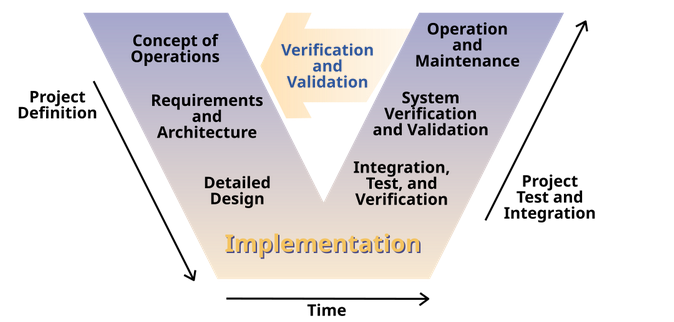
\includegraphics[width=0.5\textwidth]{pics/v-model.png}
    \caption{V-Model of software development and testing \cite{WikiVModel}}
    \label{fig:v-model}
\end{figure}

\section{Goals and Objectives}

This project aims to eliminate all of the listed problems and concerns while building upon and improving the existing capabilites of the Script Assembler. 

\begin{itemize}
    \item \textbf{EBNF parsing:} \\
    The existing structure of the test scripts should be formed into its own EBNF language which is then integrated into the Script Assembler. This eliminates a majority of the hard-coded parts of the software. Furthermore the editor should provide appropriate syntax highlighting when writing or editing a test script.

    \item \textbf{Keyword support:} \\
    New functionalities should be implemented which allows the editor of test scripts to specify aspects like the version and the operating system the test has to be run on. The structure of keywords need to be precisely set in the EBNF language.

    \item \textbf{Database mock:} \\
    The structure of the currently used TestRail database should be studied and an accurate mockup should be created. A seamless switch between the mock and the real TestRail instance has to be implemented as well.
\end{itemize}

\chapter{Used Technologies [F]}\label{chap:technologies}
\setauthor{Filip Schauer}
Just like the \gls{trp} project for which this project aims to provite an extension for, it was mainly written in the Python programming language. Aside from that, other tools have also been used or are otherwise important to be mentioned. The goal of this section is to give a broad overview of each of the technologies that we utilized or otherwise worked with when having written our project. 

\subsection{Python}

Python is a high-level, interpreted, dynamically typed object oriented programming language with a focus on allowing programmers to create applications, scripts, or connections between existing programs, quickly.\cite{py-summary}


% ==========================================
% PART II: KEYWORDS
% ==========================================
\part{Keywords [F, X, A]}\label{part:keywords}

\chapter{Keywords Specification [F]}\label{chap:keywords-specification}
\setauthor{Filip Schauer}
% !TEX root = ../../thesis.tex

In programming, a \textit{keyword} is a predefined word with a reserved meaning. Keywords can generally not be used for any other purpose, and they make up a programming language's syntax~\cite{keyword}.

In our Script Assembler, we use custom keywords in a similar way, although it may be difficult to define whether or not it is useful to refer to our parser's syntax as a \textit{programming language}. 

In this chapter, the term \textit{whitespace} is defined to refer to any amount of space or tab characters. Here, for convenience, line-breaks are chosen to specifically not fall under said definition.

\section{Robot files}

In the \gls{trp} project, the Robot Framework provides the primary scripting language that makes up the tests to be run on KeTop devices. 

A Robot file contains so-called \textit{test cases}, which are blocks commonly made up of a few lines of code~\cite{robot-framework}. Despite most parts of the syntax being irrelevant to the Script Assembler's workings, in order to get a feel for the nature of this project it may still be useful to have a look at an example of a Robot script file as is seen in Listing~\ref{lst:robot_example_script}, which is taken from Robot Framework's official home page:

\begin{lstlisting}[caption={Example code of a Robot script file~\cite{robot-framework}.}, label={lst:robot_example_script}]
*** Settings ***
Documentation     A test suite for valid login.
...
...               Keywords are imported from the resource file
Resource          keywords.resource
Default Tags      positive

*** Test Cases ***
Login User with Password
    Connect to Server
    Login User            ironman    1234567890
    Verify Valid Login    Tony Stark
    [Teardown]    Close Server Connection

Denied Login with Wrong Password
    [Tags]    negative
    Connect to Server
    Run Keyword And Expect Error    *Invalid Password    Login User    ironman    123
    Verify Unauthorised Access
    [Teardown]    Close Server Connection
\end{lstlisting}

As is made clear from the example above, some lines may be preceded by whitespace. Since the Robot Framework achieves nesting by having lines be preceded by an integer multiple of exactly four spaces certain lines of code may be syntactically erroneous or interpreted differently when that amount of whitespace is changed~\cite{robot-framework-style-guide}. This is an example of a programming convention that in this thesis will be referred to as \textit{significant indentation}. Python, for instance, works in a similar way, requiring a predefined use of leading whitespace to achieve grouping of statements~\cite{py-indentation}.

Despite Robot Framework's general ease of use, proficient support for extensibility, and versatile testing capabilities, the control over the specific execution flow is limited~\cite{robot-framework-pros-cons}. In the context of \textit{KEBA Group AG}, a single \textit{KeTop} may need to run multiple Robot script files, and a Robot script file may need to be reused for multiple KeTops. However, since it may be required for a test to be made of a single script file, it might be necessary to \textit{stitch together}, or in other words to concatenate, the contents of multiple Robot script files into one. 

Without the Script Assembler, a user may run into issues where they, for instance, would like a certain piece of code to only be included on KeTops satisfing a certain condition like being of a predefined operating system, or for certain pieces of code to be executed at a time that is either before or after the remaining parts, as the Robot Framework may not provide a useful way to achieve the required flow. 

\section{What Keywords Are}

Our project allows for custom keywords, all of which being preceded by the \verb|@| character, to be defined to act as either \textit{options} or \textit{modifiers}. In a provided file, these keywords must be defined at the start of the line, optionally preceded by indentation for nesting purposes. Lines containing such valid keywords will not be included in the concatenated output file. 

A keyword may be defined to have either no or any number of optional or required arguments. If set, these arguments may then consist of any sequence of characters without line-breaks that is prefixed by the keyword with at least one whitespace inbetween. 

The difference between options and modifiers lies in that options do not include a \textit{block body}, while modifiers do. A \textit{block body} is defined to be made up of all lines of text that, when read from top to bottom, succeed the line of the keyword, up until and not including the first line that is found that does not include at least one additional level of indentation than that of the line of the keyword, or up until the end of the file, ignoring all lines that are either empty or are solely made of whitespace. The \textit{scope} of the block body refers to the parts of the code that belong to it, as opposed to the parts of the code that do not. A level of indentation is defined to be made up of either four spaces or one tab character. 

To make up for the extra level of indentation used to define the span of the body text, the parsed body text will be stripped of that one line of indentation. Non-keyword lines, and lines that do not belong to the block body of a modifier will simply be ignored by the Script Assembler and will thus be appended into the output Robot file as-is. This means that, if the provided file does not contain anything that may be matched as a keyword, the parser should leave it as-is, aside from possible minor whitespace changes. In the case of a valid Robot file, this may only not be the case in rare exceptions, as the \verb|@| character is generally not utilized in Robot files that are to be executed on a KeTop.

\section{Examples}

\subsection{Options}

For instance, take the following code snippet, which includes the option \verb|@NO_KETOP|, which takes no arguments:

\begin{lstlisting}[caption=Example of an Option before parsing., label={lst:option_example_before_parser}]
@NO_KETOP
Install MS
\end{lstlisting}

When the line containing \verb|@NO_KETOP| is encountered, the \verb|no_ketop| flag, for which the concrete behaviour is explained in Chapter~\ref{chap:keywords-list}, is enabled for the output script. Since that specific line will not be included in the output script, assuming Listing~\ref{lst:option_example_before_parser} to be the only input to the parser, the output file may look like the following:

\begin{lstlisting}[caption={Parser result of Listing~\ref{lst:option_example_before_parser}.}, label={lst:option_example_after_parser}]
Install MS
\end{lstlisting}

\subsection{Modifiers}

Another example is using the modifier \verb|@VERSION|:

\begin{lstlisting}[caption=Example of a Modifier before parsing., label={lst:modifier_example_before_parser}]
Execute on Ketop    echo A
@VERSION BIOS > 1.0.1
    IF    ${SINGLE_MODE} is $False
        Execute on Ketop    echo B
    END
Execute on Ketop    echo C
\end{lstlisting}

Here, the line two, which is made up of \verb|@VERSION BIOS > 1.0.1|, represents a boolean condition relating to the version of the KeTop device. The block body of this condition is made up by the lines three to five. According to the specification of the \verb|@VERSION| keyword, that block body will be included only if the condition stated in its argument is satisfied.

This means that, again assuming Listing~\ref{lst:modifier_example_before_parser} to be the only input to the parser, if the condition \verb|BIOS > 1.0.1| is satisfied, the output may look like the following:

\begin{lstlisting}[caption={Parser result of Listing~\ref{lst:modifier_example_before_parser} if the condition is met.}, label={lst:modifier_example_after_parser_condition_met}]
Execute on Ketop    echo A
IF    ${SINGLE_MODE} is $False
    Execute on Ketop    echo B
END
Execute on Ketop    echo C
\end{lstlisting}

Note the removal of one level of indentation of what used to be the block body. If, instead, the case of the condition is not satisfied, the output may instead be:

\begin{lstlisting}[caption={Parser result of Listing~\ref{lst:modifier_example_before_parser} if the condition is not met.}, label={lst:modifier_example_after_parser_condition_not_met}]
Execute on Ketop    echo A
Execute on Ketop    echo C
\end{lstlisting}

\section{Recursion}

Keywords may also be defined recursively. Recursion is generally defined as being \textit{the process in which a function calls itself directly or indirectly}~\cite{recursion}. In the case of the Script Assembler, it refers to the fact that block bodies of modifiers may also include modifiers, of which the block bodies may then also include modifiers, and so forth. To show this possibility, consider the following example:

\begin{lstlisting}[caption={Example of modifiers being defined recursively.}, label={lst:recursive_modifier_example}]
@BRACKETSTART
    @OS WIN10
        @VERSION BIOS >= 1.7.0
            Upload Script To KeTop    E2Speed.ps1
\end{lstlisting}

Here, the block body of \verb|@BRACKETSTART| is made up of lines two to four, of which the block body of \verb|@OS| is made up of lines three and four, of which the block body of \verb|@VERSION| is made up of line four. Despite the order of \textit{which blocks are nested inside which} not making a difference with how all existing modifiers are specified, in general, the parser will interpret this from the outside to the innermost level of nesting, similar to how nesting is handled by most ordinary programming languages. 

This means that, if the above snippet is the only input file that contains the \verb|@BRACKETSTART| keyword, given how that keyword is specified, the part of the output script that is the so-called \textit{bracket start} will be: 

\begin{lstlisting}[caption={Bracket-start parser result for Listing~\ref{lst:recursive_modifier_example} for satisfied conditions.}, label={lst:bracket_start_output_example}]
Upload Script To KeTop    E2Speed.ps1
\end{lstlisting}

In the case of both of the conditions from the respective specifications of the \verb|@OS| and \verb|@VERSION| keywords and with each of their respective arguments being met. Otherwise, the \textit{bracket start} of the output file will be empty. 

\section{Concatenation and Output}

In general, the files get concatenated in the same order that they are given, unless keywords that change that predefined flow are used. Then, to assure the final output Robot file is valid and executable on a KeTop, the following template code will be appended before the output of the entire parsing and concatenation operations:

\begin{lstlisting}[caption={Output file template appended before inserted test cases.}, label={lst:output_template_example}]
# Template file for HMI Automation
*** Settings ***
Resource          ../../../Robot/Resources/keywords.resource
Resource          ../../../Robot/Resources/variables.resource
Suite Setup       KeTop Suite Setup
Suite Teardown    KeTop Suite Teardown
Test Setup        KeTop Test Setup
Test Teardown     KeTop Test Teardown

*** Test Cases ***
# Here the test cases are inserted
\end{lstlisting}

Finally, the resulting code will be written to a file which will then be further handled to be run either locally or on a KeTop. 

\chapter{The Different Keywords [X]}\label{chap:keywords-list}
\setauthor{Axel Csomány}
This section aims to provide a comprehensive list of keywords and their corresponding definitions and uses in the context of the Script Assembler. 

\section{Options}

Options are one of the two types of keywords that can be used within a script. They are used to set specific parameters or configurations for the specific script execution, essentially acting as flags that modify certain behaviors when dealing with the script. It doesn't require a value to be assigned to it, so its presence alone is enough to trigger the intended effect. The position of the option keyword within the script is not crucial, so it can be placed anywhere within the script while keeping its intended effect intact.

During the making of the project, one option keyword has been implemented: 

\subsection{Option: NO\_KETOP}

The NO\_KETOP option keyword can be used by typing the following line anywhere within the script:

\begin{verbatim}
    @NO_KETOP
\end{verbatim}

If this option keyword is present, the "no\_ketop" flag will be set for the entire script. This ensures that certain components that check if a KeTop device is connected are disabled, allowing the script to run without the prerequisite of a KeTop device. This is most useful for specific test scripts that have to be run without a KeTop, like installation scripts. 

\section{Modifiers}

Modifiers are the second type of keywords that can be used within a test script. They differ from options in that they require a body, specified by the presence of indentation, to function properly. The body of a modifier contains further lines of the test script, the modifier keyword itself defines under what conditions the body should be included in the final script. Generally speaking, modifiers are used to either conditionally include or exclude certain parts of the script, or set them in a specific order. 

Bodies of modifiers can also contain other modifiers, allowing the creation of complex and more specific test scripts. 

During the making of the project, the following modifier keywords have been implemented:

\begin{itemize}
    \item VERSION
    \item OS
    \item BRACKETSTART and BRACKETEND
    \item PREAMBLE
\end{itemize}

\subsection{Modifier: VERSION}

The VERSION modifier keyword can be used following the syntax:

\begin{verbatim}
    @VERSION <component> <comparison> <version>
        <body>
\end{verbatim}

Where:
\begin{itemize}
    \item \textbf{<component>} is the label of the component that is being checked, for example "BIOS".
    \item \textbf{<comparison>} is a comparison operator, such as ">", "<", ">=", "<=", "==" or "!=".
    \item \textbf{<version>} is the version of the component that the test script is being run on, in the format of "X.Y.Z" where X, Y and Z are integers.
\end{itemize}

If the version modifier keyword is present, the body of the modifier will only be included in the final script if the condition concerning the component version is met. This allows for the creation of test scripts that behave differently based on the component version of the device. 

\subsection{Modifier: OS}

The OS modifier keyword can be used following the syntax:

\begin{verbatim}
    @OS <os>
        <body>
\end{verbatim}

Where:
\begin{itemize}
    \item \textbf{<os>} is the label of the operating system that is being checked, for example "WIN10".
\end{itemize}

If the OS modifier keyword is present, the body of the modifier will only be included in the final script if the device's operating system matches the specified system. 

\subsection{Modifier: BRACKETSTART and BRACKETEND}

The BRACKETSTART and BRACKETEND modifier keywords do not require any parameters, only the keyword itself and its body:

\begin{verbatim}
    @BRACKETSTART
        <body>

    @BRACKETEND
        <body>
\end{verbatim}

If a script containing a BRACKETSTART or BRACKETEND modifier keyword is being run together with other test scripts, the body of these modifiers will be run before and after the content of all other test scripts respectively. If a batch of test scripts contains multiple scripts containing these modifiers, the bodies of the modifiers will be run in the order they appear in the batch, meaning that the body of the first BRACKETSTART modifier will be run before the body of the second BRACKETSTART modifier. The same principle applies to the BRACKETEND modifiers.

Therefore, these modifiers can be used to set up tests that require a certain amount of time to have passed, before the result can be observed. For example, if a test script is meant to check the behavior of a device after it has been active for 30 minutes, the BRACKETSTART modifier can be used to set up the test, and the BRACKETEND modifier can be used to check the results after the 30 minutes have passed. In the meantime, other test scripts can be run between the two "bracket tests", allowing for a more efficient use of time when running a batch of test scripts.

\subsection{Modifier: PREAMBLE}

The PREAMBLE modifier keyword can be used following the syntax:

\begin{verbatim}
    @PREAMBLE <index>
        <body>
\end{verbatim}

Where:
\begin{itemize}
    \item \textbf{<index>} is an integer that specifies the order in which the preambles are run, with 1 being the first preamble to be run.
\end{itemize}

When one or multiple test scripts containing a PREAMBLE modifier keyword is being run together with other test scripts, the body of the PREAMBLE keyword will be run before the content of all other test scripts, including lines in the body of a BRACKETSTART modifier. In the case of multiple PREAMBLE modifiers being present in the batch of test scripts, the bodies will be run in the order of their specified index.

The PREAMBLE modifier can be used to write scripts that test certain installation processes and their successful completion before the rest of the test scripts are run.

\section{Visual Example}

Consider the following diagram:

\begin{figure}[ht]
    \centering
    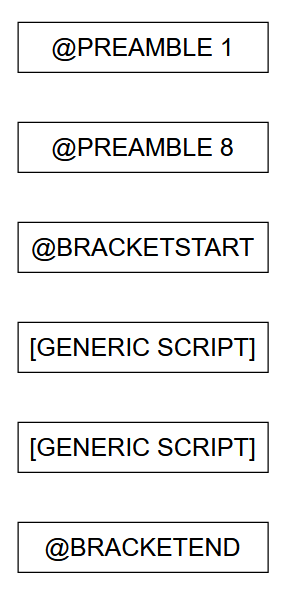
\includegraphics[width=0.35\textwidth]{pics/script-order.png}
    \caption{Simple Diagram depicting the order scripts with a certain modifier keyword are run in.}
    \label{fig:script-order}
\end{figure}

Here, it can be seen how some specific test scripts are arranged in the final script.

\begin{enumerate}
    \item The bodies of the PREAMBLE modifiers are ordered first if present. In the case of multiple PREAMBLE scripts being present, the specified index is used to order them accordingly. As seen in the diagram, leaving out certain indices doesn't lead to any issues, the ordering occurs as intended.
    
    \item The bodies of the BRACKETSTART modifiers are ordered next if present. In the case of multiple BRACKETSTART scripts being present, the order they appear in the batch is maintained.
    
    \item At this point, the content of all test scripts not containing any order-modifying keywords are placed. Their order is determined by the order they appear in the batch.
    
    \item Lastly, the bodies of the BRACKETEND modifiers are ordered if present. In the case of multiple BRACKETEND scripts being present, they follow the same principle as the BRACKETSTART modifiers, meaning that the order they appear in the batch is maintained.
\end{enumerate}

% ==========================================
% PART III: EBNF
% ==========================================
\part{EBNF [A, F]}\label{part:ebnf}

\chapter{Overview of EBNF [A]}\label{chap:ebnf-overview}
\setauthor{Adam Höllerl}
% !TEX root = ../../thesis.tex

\section{Motivation for Formal Syntax Descriptions}

To be able to run tests automated on every kind of KeTop, there is a need to modify test scripts depending on the given environment. That is why an extended Robot Framework language was needed. The Extended Backus-Naur Form (EBNF) was chosen for this, to make this new language easily extendable and deterministic to implement if adopted by other developers.

In practice, in the field of computer science, it is clear that a precise description of a language is the most important foundation. It is therefore essential that applications, communication protocols or programs function according to clear syntactic rules so that they are always interpreted in the same way by humans and machines. Natural language provides many different ways of describing something. There are ambiguities in language, and these can lead to errors in interpretation. These findings are not new. They have been known for a long time. Nevertheless, there is still no common standard that everyone adheres to, especially when languages have been implemented independently by different developers~\cite[p.~V]{ISO/IEC149771996InformationBNF}.

Syntactic metalanguages exist to solve this problem. The goal of a metalanguage is to describe another language. This means there is a difference between the language that is described and the language used to describe it.

In programming, a metalanguage is a language used to describe the syntax and structure of another language, called the object language. For example, BNF and EBNF are metalanguages used to define programming languages such as ALGOL. The structure of sentences and expressions in a metalanguage can be defined using a so-called metasyntax. For example, one could indicate that the word ``noun'' can itself function as a noun in a sentence by writing: ``noun'' is a \texttt{<noun>}~\cite{WikipediaMetalanguage}.


\section{The Backus-Naur Form (BNF)}

One of the most important metalanguages for programming has been BNF (the so-called Backus-Naur Form). BNF started with ALGOL 60 in 1960. ALGOL 60 needed a clear, formal way to describe its syntax. John Backus and Peter Naur therefore created BNF. It made it possible to define language rules precisely. This was the first time syntax was described formally. The history of ALGOL 60 is crucial because it gave BNF its first real use. BNF became the foundation for defining many programming languages. It is still essential in compilers and language design today~\cite[ p.~3]{Mossenbock2025}.

As BNF was first used for ALGOL 60 and became the model for many later languages, over time, people added changes or extensions, which created some confusion. Despite this, BNF showed the importance of clear, formal syntax.

Therefore, Extended BNF was later developed from BNF and included the most common extensions. The large amount of variants motivated the standardization effort that resulted in the standard named \emph{ISO/IEC~14977} by the International Organization for Standardization~(ISO)~\cite[p.~V]{ISO/IEC149771996InformationBNF}.

\section{The Evolution to Extended BNF (EBNF)}

For early programming languages such as ALGOL 60, BNF was adequate. However, the increased complexity of modern languages required a more systematic notation to describe their syntax effectively.

Therefore, the so-called Extended Backus-Naur Form (EBNF) was introduced. The inventor of Extended BNF - EBNF, is Niklaus Wirth, a Swiss computer scientist. EBNF is based on BNF but it adds more elements.

\begin{quote}
``One cannot fail to notice the lack of "common denominators."''~\cite{Wirth1977WhatDefinitions}
\end{quote}

Niklaus Wirth stated this in his first article in the journal ``Communications of the ACM'' in 1977 about EBNF.

He explained that there is a lack of common standards or unified fundamental principles across different language definitions and notational forms. Each language definition tends to use slightly different variants of the Backus-Naur form based notation. There is no generally accepted standard, and the differences are often small but unnecessarily varied. He stated that a more uniform notation would improve scientific work and comparison. EBNF is his solution for this problem. 

As mentioned EBNF is clearly based on BNF, but it adds more elements. EBNF can define exact numbers of elements, describe exceptions, add comments, use flexible rule names, and allow extensions. This makes grammar definitions shorter and it is easier to read them. But EBNF also has restrictions. It can only handle languages with elements in order and is not able to describe very complex grammar~\cite[pp.~VII-VIII]{ISO/IEC149771996InformationBNF}.

The main disadvantage of BNF according to ISO/IEC~14977 was:

\begin{quote}
``Backus-Naur Form (used in ALGOL 60) has problems if the metasymbols \texttt{< > ::=} occur in the language being defined. Some common forms of construction (e.g.\ comments) cannot be expressed naturally; other constructions (e.g.\ repetition) are long winded.''~\cite[p.~VII]{ISO/IEC149771996InformationBNF}
\end{quote}


The added advantages, but also the limitations of EBNF, will be discussed in more detail in later sections and chapters.

\section{Wirth's Approach to Syntax Definition}

Having established the historical need for a unified standard in the previous section, it is now necessary to examine the concrete syntactic rules proposed by Niklaus Wirth in 1977. In his article published in the journal Communications of the ACM (CACM), Wirth addressed the existing problems of syntactic notation directly. His contribution marked an important step in the formal development of language definitions.

Wirth did not intend to introduce a completely new theoretical concept. Instead, his objective was to improve the existing Backus-Naur Form in a systematic way. BNF had already proven to be useful. However, it contained ambiguities and practical limitations.

The notation presented in his article was therefore designed to be more practical and clearer in structure. It focused on improving readability and standardization rather than expanding theoretical expressive power. The goal was not innovation for its own sake. The goal was clarity, consistency, and easier application in real technical environments.

Wirth listed the following properties to extend BNF~\cite{Wirth1977WhatDefinitions}:

\begin{enumerate}
    \item The notation clearly separates meta symbols, terminal symbols, and nonterminal symbols. \\
    Example: \texttt{syntax = "production".} \\
    Here, \texttt{syntax} is a nonterminal symbol. \texttt{"production"} is a terminal symbol. The equals sign and the dot are structural meta symbols.
    
    \item Symbols used for structure can also be used as normal language symbols. This avoids artificial restrictions. \\
    Example: If quotation marks are used as meta symbols, they can still appear inside text if written twice, like \texttt{""} in many programming languages.
    
    \item The notation contains a simple way to express repetition. This reduces the need for recursion in simple cases.
    
    \item The notation avoids explicit representation of the empty string, such as by using \texttt{<empty>} or $\varepsilon$.
    
    \item The notation is based on the \gls{ascii} character set. This makes it easy to use in most technical environments.
\end{enumerate}

In his article, he showed the power of EBNF by defining its own syntax as an example (see Figure~\ref{fig:defebnf}):

\begin{quote}
``This meta language can therefore conveniently be used to define its own syntax, which may serve here as an example of its use. The word identifier is used to denote nonterminal symbol, and literal stands for terminal symbol. For brevity, identifier and character are not defined in further detail.''\cite{Wirth1977WhatDefinitions}
\end{quote}

\begin{figure}[h]
    \centering
    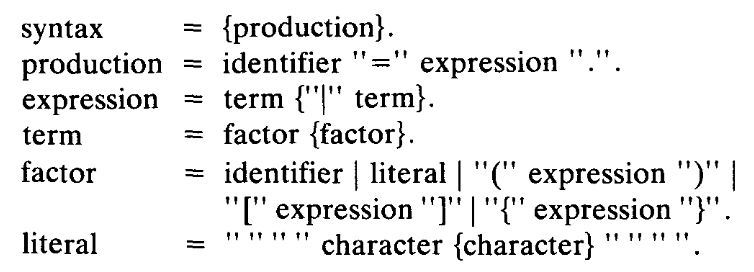
\includegraphics[width=0.75\linewidth]{pics/Definition_of_EBNF_in_EBNF.png}
    \caption{Definition of EBNF in EBNF in ``What Can We Do about the Unnecessary Diversity of Notation for Syntactic Definitions?'' from N. Wirth~\cite{Wirth1977WhatDefinitions}}
    \label{fig:defebnf}
\end{figure}


\section{Core Syntactic Extensions}

The following overview focuses in more detail on the differences between BNF and Extended Backus-Naur Form (EBNF) as described in Concepts of Programming Languages by Robert W. Sebesta~\cite[pp.~149-151]{SebestaConceptsEdition}.

It is worth noting that these extensions do not add to the descriptive capabilities of BNF. Their purpose is simply to make formal grammars easier to read and write. BNF is theoretically sufficient for describing context-free languages, but EBNF provides a more concise notation for complex structures.

\subsection{Core Syntactic Extensions in EBNF in detail}

Sebesta identifies three primary extensions common to most versions of EBNF:

\begin{itemize}
    \item \textbf{Optionality} (\texttt{[...]}): \\
    Brackets are used to denote a part of a right-hand side (RHS) that may occur once or not at all. \\
    Example: \texttt{[meow]} means meow or empty.
    
    \item \textbf{Repetition} (\texttt{\{...\}}): \\
    Braces indicate that the enclosed part can be repeated any number of times, including zero. This replaces the need for recursion when describing simple lists. \\
    Example: \texttt{\{chirp\}} can be empty, chirp, chirpchirp, chirpchirpchirp, and so on. \\
    Example for the usage for lists: \texttt{list = <item> \{<item>\}}, which represents a list of one or more items.
    
    \item \textbf{Multiple-Choice Options} (\texttt{(...|...)}): \\
    A set of alternatives can be written in parentheses, with the vertical bar (i.e., the OR operator \texttt{|}) used to separate the possible choices. \\
    Example: \texttt{(pancake | waffle)} represents either pancake or waffle.
\end{itemize}

In this notation, brackets, braces, and parentheses serve as metasymbols rather than terminal symbols of the language being described~\cite[pp.~149-151]{SebestaConceptsEdition}.

\subsection{Further Syntactic Extensions in EBNF based on ISO/IEC 14977}

However, there are more differences between BNF and EBNF in the ISO/IEC 14977 definition:~\cite[p.~VII]{ISO/IEC149771996InformationBNF}

\begin{itemize}
    \item \textbf{Defining an explicit number of items:} In some cases it is needed to describe, that e.g., a field must have an exact length. In BNF, this is difficult. Often, the programmer has explained it then informally in English. Now EBNF solves this by allowing an integer followed by a repetition-symbol (\texttt{*}). With this solution, the programmer can specify the exact number of items. This makes rules much shorter.
    
    \item \textbf{Exceptions:} Sometimes it would be easier to define a rule by specifying what is not allowed. But BNF cannot easily say ``any character except a quote''. EBNF has a solution for that. EBNF uses an except-symbol (\texttt{-}) to define rules by exclusion. This makes definitions shorter and easier. Therefore, for example, a programmer can define a group of symbols and then subtract specific exceptional cases, such as ``any character except a quote''.
    
    \item \textbf{Formal comments:} Comments are an important feature, that BNF is not offering. EBNF provides a formal way to add comments using \texttt{(*} and \texttt{*)}. And these notes do not change the machine's logic.
    
    \item \textbf{Flexible names:} In BNF, names for categories often need brackets. EBNF uses an explicit comma (\texttt{,}) as a so-called concatenate symbol to link parts of a rule. This removes the restriction that category names or meta-identifiers must be single words or enclosed in brackets, allowing for more flexible naming. It also ensures that the layout of the syntax like spaces or line breaks has no effect on the defined language.
    
    \item \textbf{Extensions:} Programmers can add their own features to EBNF. These are called ``special sequences'' and are placed between question marks (\texttt{?}). This makes the start and end of any extension very easy to find. Extensions were used several times in earlier versions of the solution presented in this thesis, but were eliminated in the final version because there was no longer a need for them.
\end{itemize}

\subsection{Comparative Notation BNF and EBNF}

While classical BNF is theoretically sufficient for describing any context-free language, it is often complicated and repetitive in practice. The main cause therefore is, that it relies, as described in the previous chapter, exclusively on recursion to express lists and optional elements. In the following illustration one can see the advantage of EBNF introducing specialized meta symbols, such as braces, brackets, and parentheses~\cite[p.~153]{SebestaConceptsEdition}.

\begin{figure}[h]
    \centering
    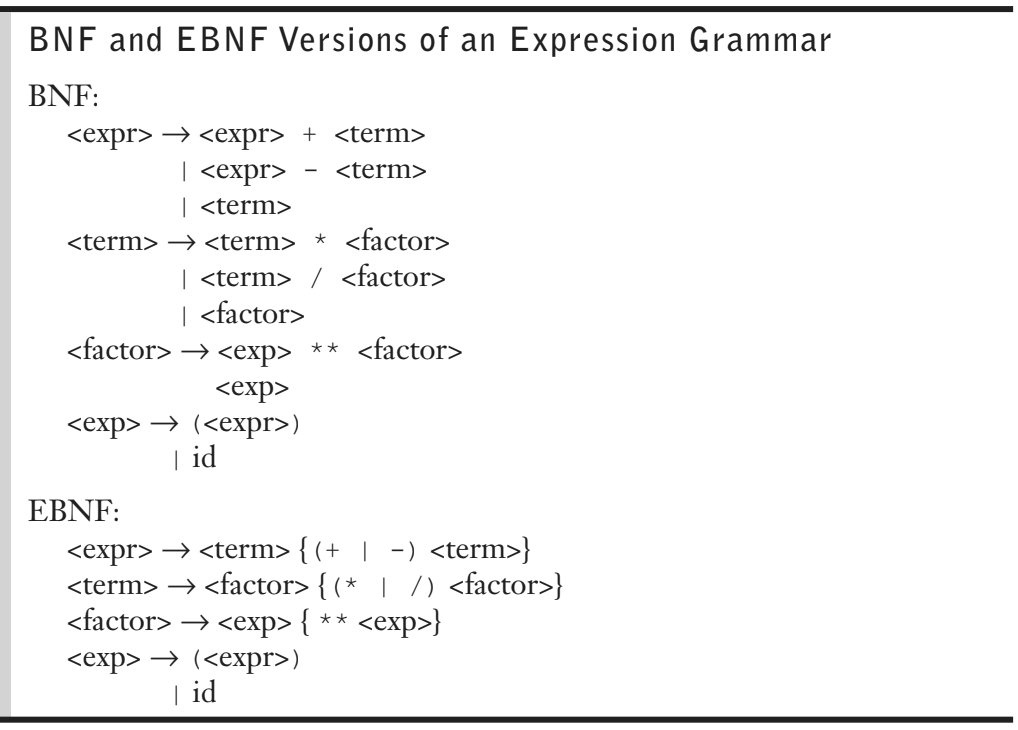
\includegraphics[width=0.75\linewidth]{pics/BNFANDEBNF.png}
    \caption{Comparison between BNF and EBNF by Sebesta~\cite[p.~153]{SebestaConceptsEdition}}
    \label{fig:bnfvsebnf}
\end{figure}


As demonstrated in the example in Figure~\ref{fig:bnfvsebnf}, the structural differences lead to a significant reduction in the number of rules required:

\begin{itemize}
    \item \textbf{Repetition via Braces in this example:} In the BNF version of the expression grammar, an \texttt{<expr>} must be defined recursively to handle a sequence of additions or subtractions. EBNF replaces this recursion with braces \texttt{\{...\}}, which denote that the enclosed part can be repeated indefinitely or left out entirely.
    \item \textbf{Multiple-Choice Options in this Example:} The example uses parentheses \texttt{(...)} combined with the OR operator \texttt{|} to group choices. This for example allows the EBNF version to handle both addition and subtraction in a single line. In BNF it requires a more complex approach.
\end{itemize}

\subsection{Modern Variations and Standardization}

While an official standard exists (ISO/IEC~14977:1996), it is rarely used in practice. There have several variations of EBNF emerged in recent years, which deviate from the standardized syntax, such as using a colon instead of an equal sign or a dot instead of a semicolon. Also the project described in this thesis partially deviates from ISO standards due to using the EBNF dialect of the Lark Python library. 

\section{ISO/IEC 14977 Standards for Assembler Logic}

While the previous chapters describe the advantages of EBNF in terms of readability and compactness, the ISO definition has an additional function. The ISO standard ISO/IEC 14977 also defines strict technical rules.

These are very important for error-free processing by an automated tool such as a script assembler, as they ensure that the grammar definition remains mathematically unambiguous.

\subsection{Operator Precedence}

For every EBNF grammar, the strictly defined hierarchy of meta-symbols is essential, as it prevents ambiguities in the rules.
The order of the symbols is clearly defined in the ISO standard without any leeway and is specified as follows: (the strongest is the repetition symbol. This takes precedence, followed by the exclude symbol, and so on).
\begin{enumerate}
\item Repetition symbol (*): For specifying exact numbers of repetitions.
\item Except symbol (-): For defining sets by exclusion.
\item Concatenate symbol (,): For explicitly linking consecutive elements.
\item Definition separator symbol (|): For separating alternatives.
\item Defining symbol (=): Formally assigns an expression to a nonterminal.
\item Terminator symbol (;): To clearly mark the end of a production rule.
\end{enumerate}

\cite[p.~1]{ISO/IEC149771996InformationBNF}

\subsection{Layout Neutrality Through Gap Separators}

Ideally, a script assembler should be able to process scripts regardless of their visual formatting. The ISO standard is helpful here, as it defines so-called ``gap separators'' (such as spaces, tabs, or line breaks)~\cite[pp.~5]{ISO/IEC149771996InformationBNF}. These characters have no formal meaning outside of terminal strings. This has the significant advantage of allowing for flexible grammar design without affecting the assembler's logic. Since gap separators and comments have no formal effect on the defined language, the script assembler can ignore these characters during analysis, which, for example, increases its robustness against different programming styles.

In summary, several advantages arise. The grammar definition remains mathematically consistent for automated tools. Furthermore, it is beneficial that the grammar can be made more readable and understandable for human readers through formatting and annotations.

\subsection{Syntactic Exceptions}

As mentioned earlier, the Except symbol (\texttt{-}) allows the assembler to define specific instruction sets. An example of this would be ``all characters except a semicolon.'' However, the ISO standard also imposes very clear technical limitations on this function, as otherwise paradoxes could arise:

\begin{quote}
``If a syntactic exception is permitted to be an arbitrary syntactic factor, Extended BNF could define a wider class of languages than the context-free grammars, including attempts which lead to Russell-like paradoxes... Such a license is undesirable and the form of a syntactic exception is therefore restricted to cases that can be proved to be safe.''~\cite[p.~2]{ISO/IEC149771996InformationBNF}
\end{quote}

A good explanation for the Russell Paradox, formulated by Bertrand Russell, is the so-called barber's example: In a village, the barber shaves precisely all the men who don't shave themselves, and only these men. The question of whether the barber shaves himself leads directly to a contradiction: If he shaves himself, he shouldn't, by definition; if he doesn't shave himself, he should~\cite{WikipediaBarbierParadoxon}.

This example illustrates that such self-referential definitions can lead to logical inconsistencies in formal systems.


\subsection{Alternative Representations for System Compatibility}

To guarantee that a grammar functions on different systems, the ISO standard allows the substitution of certain special characters if they are missing. For example, the characters \texttt{(:} and \texttt{:)} can replace \texttt{\{} and \texttt{\}}, or a period (\texttt{.}) can replace a semicolon at the end of a rule. This ensures that the grammar remains readable and functional on different platforms without losing its original structure~\cite[p.~5]{ISO/IEC149771996InformationBNF}.

\subsection{Special Sequences as a Formal Interface for Assembler Extensions}

Although special sequences were already described in the previous section as a general extension option, they are listed again here to specifically clarify their ``technical'' role as placeholders. In the logic of a script assembler, they serve as a standardized mechanism to mark parts of the language that cannot be defined by EBNF itself (e.g., specific character sets)~\cite[p.~VII]{ISO/IEC149771996InformationBNF}.

By enclosing them in question marks (\texttt{?...?}), the grammar remains formally valid for the assembler tool. In this work, they thus can provided the flexibility for possible future functional extensions without violating the fundamental syntactic rules of the ISO standard~\cite[p.~3]{ISO/IEC149771996InformationBNF}.


\subsection{Evaluating the Standard for our Script Assembler}

After introducing the theoretical foundations of EBNF, it is necessary to evaluate how the ISO standard was applied in the context of the script assembler. The goal of the project was not to implement a complete parser for the Robot Framework. Instead, the focus was on building a preprocessor for specific control tags such as \texttt{@OS}. For this reason, the resulting grammar is not a strict implementation of the ISO standard. It represents a pragmatic combination of formal rules and practical requirements.

A central aspect of this evaluation is the concept of layout neutrality. The ISO standard defines spaces, tabs, and line breaks as so-called gap separators. These elements have no formal meaning and can be ignored by the parser. This principle improves flexibility and readability. However, it could not be applied completely in this project. Inline spaces and tabs between control tokens are treated as insignificant and are therefore ignored. This allows test scripts to remain flexible in their formatting.

Line breaks, however, require a different treatment. Robot Framework scripts are structured line by line. This means that line breaks carry semantic meaning. They define the structure of the script. Therefore, line breaks could not be treated as layout-neutral elements. Instead, they were explicitly defined as structural tokens in the grammar. This is a necessary deviation from the ISO specification to ensure correct processing of the input.

Further deviations from the standard were made in the handling of syntactic constraints. The ISO standard introduces syntactic exceptions to define rules by exclusion. However, this mechanism can become complex and difficult to understand. In some cases, it can even lead to problematic definitions. For this reason, syntactic exceptions were not used in the assembler.

Instead, the implementation relies on regular expressions. \Gls{regex} provides a practical way to capture and process text patterns. It allows the parser to treat sections of Robot Framework code as plain content. The internal structure of these sections is not analyzed. This simplifies the grammar and reduces its complexity. As a result, the grammar becomes easier to read and maintain.

\chapter{Approaches to EBNF [A]}\label{chap:ebnf-approaches}
\setauthor{Adam Höllerl}
% !TEX root = ../../thesis.tex

\section{Requirements}

When creating new formal grammar, one quickly is confronted with a common problem in software development. On one side, you want a clean design, but on the other there is this old legacy system at the company that everyone is used to. For the development of the Script Assembler, this means that it must not only be able to process multi-line structures correctly, but also that the legacy system used at KEBA must continue to function with the new formal grammar, and unfortunately, backward compatibility is a must-have.

The legacy system used before the Script Assembler is a simple preprocessing system, that was based on basic string matching. This solution uses markers that start with an \texttt{@} sign. Those were already existant:
\begin{itemize}
    \item \textbf{\texttt{@BRACKETSTART}, \texttt{@BRACKETEND}:} These strings marked sections of code. The system just checked if a line exactly matched these strings to know if the following Robot Framework code should be appended at the beginning or the end of the final script.
    \item \textbf{\texttt{@NO\_KETOP}:} This was a global option that meant a KeTop device was not needed for the test. It could be written anywhere in the file, and the script just searched the whole document for it without looking at the context.
\end{itemize}

This solution checked if a specific string was present inside a file or a line and did not use a formal parser. This worked fine for isolated, simple use cases, but not with complex, context-sensitive multi-line structures or dynamic block delineations. Without a parser, the hardcoded logic simply becomes an unmaintainable mess over time.

For this reason, designing the new formal grammar became hard to manage, because three major restrictions had to be taken into account, as clarified in the first meetings by KEBA:
\begin{itemize}
    \item \textbf{Deterministic Parsing:} The system needs strict, unambiguous rules to cleanly differentiate syntactic constructs and reliably deal with multi-line scopes. 
    \item \textbf{Backward Compatibility:} It was a strict requirement that the old legacy scripts kept working exactly like before. The functionality had to be preserved. A disruption of the established workflow for the testing team was not an acceptable option.
    \item \textbf{Future Extensibility:} The system must be very robust, because it was stated, that new custom annotations and hardware-specific conditions will definitely be added in the future. A complete rewrite of the parser for every new feature would simply not be an option.
.
\end{itemize}
The testing team at KEBA was already deeply familiar with the \texttt{@} prefix. Early design discussions brought up the idea to introduce distinct prefixes to simplify the parsing. The suggestion was to introduce \texttt{\#} for global options, and \texttt{\&} for block statements. The idea was, that the tokenization process would become significantly easier and more accurate this way. The evaluation feedback then showed the problem that the distinct prefixes break all existing test suites. A complete disruption of the developers workflow would be the result.

 This created a conflict. A new parser is strictly necessary, but the legacy \texttt{@} prefix and the overall backward compatibility must still remain intact. This conflict dominated the first design phase and led to the following solution. Though the strictness of the ``Backward Compatibilty'' restriction was not as clear at that point.
 To establish a good understanding of the available options and technical trade-offs, two contrasting EBNF approaches were modeled. The evaluation happened before the final syntax design was established.


\section{Minimal EBNF Approach}

One of the two strategies explored was the minimal EBNF approach. The idea behind this specific design was to capture the general script structure as broadly as possible. Theoretically, this offers maximum flexibility and makes future extensions very easy.

Listing~\ref{lst:minimal_ebnf} demonstrates this broad structural definition. The grammar does not strictly define every possible keyword. Instead, it simply distinguishes between standard Robot Framework lines, single-line operators, and multi-line operators. 


\begin{lstlisting}[caption={The Minimal EBNF grammar}, label={lst:minimal_ebnf}, float=htbp]
script = {line, nl}, [line].
line = robot | operator | multiline_operator.
robot = ? robot code line ?.
operator = '@', word, { ws, argument }.
multiline_operator = operator, [nl], '{' { robot, nl } '}'.
nl = "\n".
ws = " " | "\t".
argument = ? some argument for example comparison operators or strings ?.
\end{lstlisting}

\subsection{Problems of the Minimal Approach}

While the parser implementation stays lightweight and adaptable with this approach, there is a blind spot and it completely fails at validating the actual code structure:
\begin{enumerate}
    \item \textbf{Unresolved Ambiguities:} The grammar failed to strictly define and categorize specific keywords. It could not differentate between standalone options (e.g., \texttt{@NO\_KETOP}) and block-defining modifiers (e.g., \texttt{@VERSION}). The parser was basically blind to the meaning of the words and no correct validation was possible.
    \item \textbf{Scope Definition Conflicts:} A critical issue emerged during the following design phases when indentation was chosen over explicit brackets (e.g., \texttt{\{} and \texttt{\}}) as the primary method for defining scopes. The minimal grammar was just defined too loosely for it to be able to differentiate between either an option that has a body despite it not being allowed to (e.g., developer misinterpreting functionality). The parser was not able to detect the syntax error and invalid code might pass through.
\end{enumerate}


\section{Detailed EBNF Approach}

While the Minimal Approach explored maximum flexibility, a completely different and rather strict grammar was developed. This EBNF approach uses clear rules and a strict separation of all constructs. The main goal was a much better parsing clarity.

As shown in Listing~\ref{lst:detailed_ebnf},  this iteration uses distinct prefixes for different types of constructs. It also introduces explicit termination symbols to make the structure clear.

\begin{lstlisting}[caption={The Detailed EBNF grammar}, label={lst:detailed_ebnf}, float=htbp]
S = { ' ' | '\t' } ;
robot_line = S , ?robot_script_line? , S ;
option_line = S , '#' , S , option , S ;
statement_line = S , '&' ,  S , statement , '\n' , { line , '\n' } , S , '&/' , S , '\n' ;
line = robot_line | statement_line | S ;
script = { option_line , '\n' } , ( ( { line , '\n' } , [line] ) | [option_line] ) ;

statement = version ;
option = "NO_KETOP" ;
section = "BRACKETSTART" | "BRACKETEND" ;

version = "VERSION" , S , ( '>' | '<' | '=' | '>=' | '<=' ) , S , ?version_number? ;
\end{lstlisting}


Looking closer at the code, on can see, that in this specific design, \texttt{\#} was introduced for global options, and \texttt{\&} was utilized for statements, which were explicitly terminated by \texttt{\&/}. Since this approach was never fully completed \texttt{@} was not used yet, but the idea was to use it only for sections. The grammar also checks the expected arguments very strictly. For instance, the \texttt{VERSION} statement forces the user to use mathematical comparison operators and a specific version number format (line 12).

\subsection{Problems of the Detailed Approach}

This approach was very precise and stable. Unfortunately, there were two severe drawbacks that made it unusable for the final product:
\begin{enumerate}
    \item \textbf{Loss of Backward Compatibility:} The introduction of \texttt{\#} and \texttt{\&} caused problems with the existing \texttt{@} prefix used by the existing option. Changing all the old code was not an option. Furthermore it seemed more intuitive to just have one prefix for all types.
    \item \textbf{Excessive Rigidity:} The rules for how an argument must look are too strict. For example, the forced mathematical operators in the \texttt{version} rule make the grammar very rigid. This means every time a new modifier is added with new arguments, the EBNF has to be updated to match the arguments exactly. This made the Script Assembler harder to extend.
\end{enumerate}

\section{Conclusion}

Testing these two different approaches provided important details for the final EBNF. The Minimal Approach showed the possible dangers of structural ambiguity. It is clear that the parser needs to ``understand'' the difference between a standalone option and a block-defining modifier. On the other hand, the Detailed Approach proved that excessive rigidity is also not completely perfect. Making the parsing process too easy for the machine just makes extending unneccessary hard.

The conclusion from this evaluation phase was that the final grammar definitely needed a hybrid design to work. On the inside, it requires the precision of the Detailed Approach, which  means in detail that all keywords must be strictly defined and categorized internally so the parser can recognize valid scopes and modifiers correctly. But at the same time, it still has to keep the same look and the backward compatibility of the old legacy approach by using the \texttt{@} prefix, everywhere, while also making the argument structure much more relaxed to make it easier to add extensions later on.

The idea of explicit termination symbols like \texttt{\&/} was completely dropped in favor of indentation-based scoping, and the old ``sections'' were just changed into standard modifiers.

The combination of all these different requirements finally leads to the final functional grammar used in Script Assembler.


\chapter{EBNF's Indentation Problem [F]}\label{chap:ebnf-problem}
\setauthor{Filip Schauer}
\section{Final EBNF Requirements}

To get to our final \gls{ebnf}, we have to represent all of the following:

\begin{itemize}
    \item The entire script is made of ``lines'', seperated by line breaks, each of which can be a ``robot line'', an ``option line'', or a ``modifier line''. 
    \item There are two different types of keywords: ``options'' and ``modifiers''. Valid ``options'' include \verb|@NO_KETOP| and valid ``modifiers'' include \verb|@VERSION|, \verb|@OS|, \verb|@PREAMBLE| \verb|@BRACKETSTART|, and \verb|@BRACKETEND|.
    \item It should be possible for both ``modifiers'' and ``options'' to have optional arguments until the end of the line. The nature of the argument itself or whether or not a specific keyword should require or allow for an argument should be, for simplicity and ease of extensibility, handled by the parser and therefore do not lie within the scope of the \verb|ebnf|. 
    \item ``Modifier lines'' include a ``block body'', which is also made up of additional ``lines'' which may be a ``robot line'', ``option line'', or, recursively, a ``modifier line''. 
    \item A block body is marked by each line of text being preceded by an indentation character, which may either be a tab character or four spaces. 
    \item All other lines are handled as ``robot lines''.
\end{itemize}

Note that in the listing above, there is a differentiation between the \gls{ebnf} object ``lines'' and the term ``line of text'', which stands for a literal string terminated by a new line charecter or the end of the file. 

However, what follows is a non-rigorous proof by contradiction that it is impossible to fully define a language that meets all the above requirements in \gls{ebnf}.

\section{Impossibility of Indentation}

What follows are three statements that, for the purposes of this non-rigorous proof, are each assumed to be true. 

Firstly, it is possible to specify the ``modifier line'' as a single, re-usable component, because it must be possible for a ``modifier line'' including its ``block body'' to refer back to itself to allow for recursion. 

Secondly, as stated in the requirements above, a ``block body'' of a ``modifier line'' may be made up of any number of lines of text, each of which should be preceded by an indentation. 

Thirdly, when a ``modifier line'' B is defined inside the ``block body'' of another ``modifier line'' A, it is possible to specify that each ``line'' of the ``block body'' of ``modifier line'' B should be preceded by indentation.

However, the third statement would require ``modifier line'' B to be defined differently to ``modifier line'' A, as each of its line of text of its ``block body'' must be predeced by an indentation as stated in the second statement. This means that, in order to require indentation as prefix for every inner ``line'', a ``modifier line'' may not allow for the same kind of ``modifier line'' as would be used in other parts of the script to be used in its ``block body'', which violates the first statement which requires ``modifier lines'' to be defined as single and re-usable components. Therefore, it is not possible for all three statements to be true at once. 

\section{A Solution}

A simple solution to this problem is to not define the entire language in \gls{ebnf}, but rather, to require a ``preprocessor'' to sanitize the input script in a way that makes it suitable for \gls{ebnf}. 

In our project, the task of the preprocessor is to transpile the indentations required for defining the scope of a block body to a more \gls{ebnf}-friendly way. 

Instead, the preprocessor uses indentation to determine the scope of a block body. Then, that indentation is stripped from all lines of the block body, and a ``special sequence of text'' is appended below the block body to specify its end. This way, the \gls{ebnf} does not have to take into account the fact that an inner block body would otherwise require every line to have a prefix. Instead, a ``modifier line'' is able to ``sandwich'' any lines in between a clear beginning (which is the line that the ``modifier'' is defined) and a clear end (which is the mentioned ``special sequence of text'').

The choice of that ``special sequence of text'' should be one that is not expected to be in the input script. For Script Assembler, we chose \verb|@END|, as we have already reserved the \verb|@| character for our purposes, there is no keyword with that name, and it still leaves for human-readable code if a user were to look at the code after the preprocessor but before parsing.

A side effect of this is that a user may be able to specify the scope of a block body using \verb|@END| as opposed to how it is defined in the specification. However, this can easily be mitigated by requiring the preprocessor to simply not allow the use of \verb|@END|. 


\chapter{Our EBNF [F]}\label{chap:our-ebnf}
\setauthor{Filip Schauer}
From the requirements above, the following code block is the final \gls{ebnf} that was settled on. In this chapter, we will go into detail about its syntax and meaning. 

\begin{lstlisting}
start = { N } , { line , { N } } ;

robot line = ? regex: /[^(@|\n)].+?(?=\n)/ ? ;

option line = "@" , option ;

modifier line = "@" , modifier , block body , "@END" ;

block body = { N } , { line , { N } } ;

line = modifier line | option line | robot line ;

modifier = allowed modifiers , [arg] ;
option = allowed options , [arg] ;

arg = ? regex: /[ \t]+[^\n]*/ ? ;

N = "\n" ;

allowed options = "NO_KETOP" ;
allowed modifiers = "VERSION" | "OS" | "PREAMBLE" | "BRACKETSTART" | "BRACKETEND" ;
\end{lstlisting}

It is important to note that ``inline whitespace'', i.e.\ sequences made up of only spaces or tabs, are ignored here. This is useful, as it significantly reduces the size and complexity of the \gls{ebnf}, since there is no need for our syntax to take whitespace into account, with the exception of ``robot lines'' and ``args'', and the library used for parsing an input defined in a grammer that resembles \gls{ebnf}, which is specified in detail in the next chapter, also allowing for the option to ignore inline whitespace. 

Additionally, it is necessary to define the specific ``allowed options'' and ``allowed modifiers'' in the \gls{ebnf}, as otherwise there would not be a easy and general way to differentiate between options and modifiers. 

\section{Its Components}

\verb|start| refers to the entire script. This name was chosen because it matches the name that our library has reserved for this purpose. It is made up of any amount of \verb|line|s and empty lines. 

A \verb|line| may either be a \verb|modifier line|, \verb|option line|, or \verb|robot line|

A \verb|robot line| is defined as being any line of text that is not empty, does not start with an \verb|@| character, and that ends with a line break character. Here, a \gls{regex} is used for this matching.

Both \verb|option| and \verb|modifier| refer to their respective allowed keywords, followed by an optional \verb|arg| (``argument''), which is defined as being a string which begins with an inline whitespace character and ends with the end of the line.

An \verb|option line| is a line starting with \verb|@| and a valid \verb|option|.

A \verb|modifier line| starts with an \verb|@| character, is followed by a modifier, then by a \verb|block body|, then by the sequence ``\verb|@END|'', which, as explained in the chapter above, is to be provided by the preprocessor. A \verb|block body| is refers to any amount of \verb|line|s, including or not including empty lines. 

\verb|N| is simply used for convenience and is defined to be a single line break character. 



% ==========================================
% PART IV: IMPLEMENTATION
% ==========================================
\part{Implementation [F, A, X]}\label{part:implementation}

\chapter{Introduction [F]}\label{chap:implementation-introduction}
\setauthor{Filip Schauer}
% !TEX root = ../../thesis.tex

In this part, explain own implementation for the Script Assembler in detail. Aside from \textit{Syntax Highlighting}, everything was written in the \textit{Python} programming language.

The following chapters belong to this part:
\begin{itemize}
    \item Chapter~\ref{chap:preprocessor}: \textit{Preprocessor}. This chapter goes over the \textit{Preprocessor}, which converts significant indentation of a \textit{modifier}'s \textit{block body} into a reserved keyword that is understood by the \textit{Parser}. In Chapter~\ref{chap:ebnf-problem}, the need for this preprocessor is explained in detail.
    \item Chapter~\ref{chap:parser}: \textit{Parser}. This chapter goes over the \textit{Parser}, which uses the \textit{Lark} library in combination with a modified form of our EBNF from Chapter~\ref{lst:our_ebnf} to recursively parse an input script to an output script and brackets. 
    \item Chapter~\ref{chap:option-modifier-format}: \textit{Option/Modifier Format}. Here, our implementation for handling the respective keywords within the parser is explained. 
    \item Chapter~\ref{chap:trp-integration}: \textit{TRP-Integration}. Since our project is used within the \gls{trp} project, we explain the changes we made to the existing project to integrate our Script Assembler.
    \item Chapter~\ref{chap:syntax-highlighting}: \textit{Syntax Highlighting}. Since the existing \gls{trp} project's \textit{Angular} frontend uses a code editor known as \textit{Monaco Editor}, we implemented \textit{Syntax Highlighting}, in other words text colorization based on keyword syntax, which we go over in this chapter.
    \item Chapter~\ref{chap:extensibility}: \textit{Extensibility}. In this chapter, we explain how the Script Assembler may be extended with additional keywords, give examples to keywords that may be useful in the future, and discuss the limits of our parser. 
    \item Chapter~\ref{chap:database}: \textit{Database}. Here, we explain the \textit{Mockup Database}, which we built to allow the project to run independently to the proprietary \textit{TestRail} system and to aid with testing.
\end{itemize}

In the \gls{trp} project, the following files and directories make up nearly the entirety of the Script Assembler and its components, where the \verb|.| directory refers to the project's root:
\begin{itemize}
    \item \verb|./TRP/broker/managers/case/script_assembler|: The core logic of the Script Assembler's preprocessor and parser is defined in this directory. It includes the following files:
    \begin{itemize}
        \item \verb|preprocessor.py|: Here, the \verb|Preprocessor| class is found alongside its logic. This file is shown and explained in Chapter~\ref{chap:preprocessor}.
        \item \verb|parser.py|: This file defines the \verb|parse_script| function, which serves as an entry point to the preprocessor and parser. This is explained in Chapter~\ref{chap:parser}. 
        \item \verb|formatter.py|: This file includes the \verb|Formatter| class, which includes the core logic of the recursive parsing mechanism of the given script in the form of a \textit{Lark} \verb|Tree| object. We explain this mechanism in detail in Chapter~\ref{chap:parser}.
        \item \verb|datatypes.py|: Data classes (i.e.\ classes with the \verb|@dataclass| annotation) that are used by the parser are found in this file and also explained in Chapter~\ref{chap:parser}.
        \item \verb|option_modifier_format.py|: This file is used by the \verb|Formatter| and specifies how each respective keyword should be handled. In Chapter~\ref{chap:option-modifier-format}, we explain the inner workings of this, and Chapter~\ref{chap:extensibility} explains how one might use this file to define keywords that may be needed in the future.
        \item \verb|parser_exception.py|: Here, two custom exceptions related to the parser can be found: \verb|ParserSyntaxError| and \verb|ParserInternalError|. They are explained in Chapter~\ref{chap:exceptions-and-warnigs}.
    \end{itemize}
    \item \verb|./TRP/common/dbfunc.py|: This file includes the \verb|DBSession| class, which implements the same functions as \verb|TRSession| of \verb|testrailfunc.py| (which is found in the same directory) in order to connect to and interact with our \textit{PostgreSQL} mockup database. Chapter~\ref{chap:database} explains this in detail.
    \item \verb|./Angular/src/app/app.module.ts|: This represents the primary configuration file for the \textit{Angular} project, which has been provided by our project partner, Martin Wieser from KEBA Group AG.\@ It includes the configuration for \textit{Monaco Editor}.\@ Chapter~\ref{chap:syntax-highlighting} explains how we expanded it to allow for \textit{Syntax Highlighting} for our keywords.
    \item \verb|./TRP/broker/managers/case/casemanager.py|: This file has been provided by our project partner, Martin Wieser from KEBA Group AG.\@ For our project, the\\ \verb|assemble_robot_script| method is important, as it was modified by us to integrate our Script Assembler into the existing \gls{trp} project, which is explained in Chapter~\ref{chap:trp-integration}.
\end{itemize}


\chapter{Preprocessor [A]}\label{chap:preprocessor}
\setauthor{Adam Höllerl}
% !TEX root = ../../thesis.tex

\section{Introduction}

As already established earlier on, the Script Assembler introduces a custom syntax added on top of the Robot Framework. It uses annotations such as \texttt{@VERSION} to control the test suit setup. To process this grammar the implementation uses the Lark parsing library~\cite{LarkGithub}. However while the chosen indentation-based syntax is very intuitive for the developers, it introduces technical difficulties for the parser.

Indentation-based scoping is context-sensitive. To find out if a line belongs to a block, the parser needs to know the indentation level of the previous annotation. That requires it that the current indentation depth is saved. While the Lark library provides its own indenter utility for parsing whitespace-scoped languages, it processes indentation globally~\cite{LarkDocsIndent}.
Because the Script Assembler has to differentate between its own language and the contained Robot Framework code, Lark's indenter would generate tokens for Robot Framework code indents which might lead to blocks that close too early.


That is why an additional preprocessing step is required before the Lark parser can evaluate the script. This step is handled by a preprocessor, whose goal is to isolate the meta-language indentation from the content-language indentation before parsing the script.


\section{Design and Transformation Rules}

\subsection{Content vs. Meta-Language Conflict}

The fundamental problem is that both languages use spaces and indentation to define logic and structure. In the Robot Framework, spaces and tabs separate keywords from arguments, and indentation marks the contents of blocks like \texttt{FOR} loops and \texttt{IF} statements, as shown with green highlights in Figure~\ref{fig:indents_highlights}.

At the same time, the Script Assembler uses indentation to determine which lines belong to a specific modifier, as shown with orange highlights in Figure~\ref{fig:indents_highlights}. This leads to the problem of having to somehow seperate those two kind of indents and thus the need for our own Preprocessor instead of the Lark Indenter.

\begin{figure}[h]
    \centering
    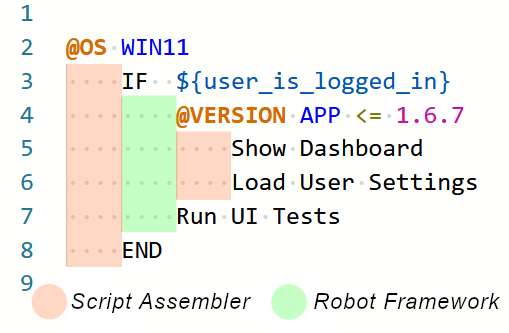
\includegraphics[width=0.75\textwidth]{pics/IndentsHighlights.png}
    \caption{Difference between meta-language and content-language indents. }
    \label{fig:indents_highlights}
\end{figure}

\subsection{Explicit Block Scoping}


To make the syntax context-free, the implicit visual scoping provided by indentation must be changed to explicit block scoping. Clear start and end markers must be defined. This is comparable to the use of curly braces \texttt{\{\}} in C\# or Java, or to opening and closing tags like \texttt{<div>} and \texttt{</div>} in HTML.


For each modifier found by the Preprocessor, the start of the block is simply the modifier itself. The end of the block, shown by a decrease in indentation in the raw script. The Preprocessor marks this by inserting the keyword \texttt{@END}.


With these clear boundaries, the EBNF grammar in Lark is simplified. It only needs to search for the \texttt{@END} token to recognize the end of a block, allowing it to completely ignore the surrounding whitespace.


\subsection{Preserving Indents}


The following example uses several annotations nested within standard Robot Framework control structures. Listing~\ref{lst:raw_script} shows a typical raw Preprocessor input script written by a test developer.


\begin{lstlisting}[caption={Raw input script with nested modifiers}, label={lst:raw_script}, float=htbp]
Setup Test Environment
    @VERSION BIOS == 1.6.1
        Log    Checking BIOS Version
        @OS WIN11
            Install Driver    audio_win11.sys
        Restart Node
\end{lstlisting}


In Listing~\ref{lst:raw_script}, a Robot Framework keyword (\texttt{Setup Test Environment}) is the root scope. Within these block, the outer Script Assembler layer performs a BIOS version check. This block contains a normal Robot command (\texttt{Log}) followed by an inner modifier that checks the operating system. This inner modifier contains a command for a driver installation. Finally, a \texttt{Restart Node} command is executed within the BIOS block, but outside the inner operating system check.


The Preprocessor should calculate the active layers of modifiers and remove only the leading indents belonging to these specific layers. Listing~\ref{lst:preprocessed_script} shows the expected output.


\begin{lstlisting}[caption={Expected Preprocesssor output}, label={lst:preprocessed_script}, float=htbp]

Setup Test Environment
@VERSION BIOS == 1.6.1
    Log    Checking BIOS Version
@OS WIN11
    Install Driver    audio_win11.sys
@END
    Restart Node
@END

\end{lstlisting}


Comparing the two listings shows perfectly how the Preprocessor is supposed to work. The modifier lines themselves (lines 2 and 4 in Listing~\ref{lst:preprocessed_script}) are completely stripped of their indentation. This is needed since the EBNF grammar only sees modifiers that begin with an \texttt{@} symbol, so if it is padded with tabs it is not recognized.

Additionally and most importantly the indentations of the contained language are preserved while the modifier indents are not. For example in the raw text the line \texttt{Install Driver    audio\_win11.sys} was indented three times. Once for the BIOS version check modifier, once for the OS check modifier and once for the actual Robot Framework block. In the result the two modifier indents are removed, leaving only the Robot Framework one.
\texttt{Restart Node}

Finally, the decrease of indentation before the \texttt{Restart Node} command triggers the Preprocessor to insert the \texttt{@END} tag and the open end adds another one lines 6 and 8 in Listing~\ref{lst:preprocessed_script}).


\section{Evolution of the Algorithm}


Developing an appropriate algorithm for this was a technical challenge. The algorithm has to correctly identify mixed indentation levels and clearly distinguish between a line that defines a new lexical scope and a line that just belongs to an existing scope. Parsing context-sensitive, whitespace-dependent meta-languages is a highly complex process, as demonstrated by the evolution of the Preprocessor logic.


\subsection{Linear Depth Counting Approach}


The first version of the Preprocessor used a simple linear mechanism for counting layers. The basic idea was that the depth of a modifier block directly correlated to a simple integer counter. 


In this naive approach, the algorithm maintained a single integer variable called \texttt{current\_layer}, starting at zero. The Preprocessor iterated through the script line-by-line, searching for the \texttt{@} symbol. When it found a modifier, it incremented the \texttt{current\_layer} counter by one. For all following lines, the algorithm removed a number of leading indents exactly equal to the value of \texttt{current\_layer}.


To find the end of a block, the algorithm compared the total number of indents on the current line against the \texttt{current\_layer} variable. If a line had fewer indentations than the active layer count the algorithm assumed that the block had ended. It then inserted an \texttt{@END} tag and decremented the counter. This logic worked in simple situations. However, it contained a fundamental flaw regarding relative and absolute indentation depths.


\subsection{Collision with the Structure of the Content}


The linear depth counting approach unfortunately failed when Script Assembler annotations were mixed with Robot Framework commands that use indents inside a modifier. At that point the absolute count of tabs of a line is no longer just determined by the Script Assembler modifier depth.

Listing~\ref{lst:problem_script} demonstrates the specific edge case that exposed the flaw in the naive algorithm.


\begin{lstlisting}[caption={Problematic edge case}, label={lst:problem_script}, float=htbp]
@VERSION BIOS == 1.2.3
    FOR    ${item}    IN    @{ITEMS}
        @VERSION KBDRIVER != 0.2.5
            Add Item To Cart    ${item}
        Sleep    0.5s
    END
\end{lstlisting}


When verifying the algorithm with Listing~\ref{lst:problem_script}, the error occurs in line 5.

\begin{enumerate}

    \item \textbf{First Modifier:} On line 1, the first \texttt{@VERSION} modifier sets the \texttt{current\_layer} to 1.

    \item \textbf{Inner Modifier:} On line 3, the inner \texttt{@VERSION} modifier increments the \texttt{current\_layer} to 2.

    \item \textbf{Conflicting Line:} On line 5, the \texttt{Sleep} command has exactly 2 leading tabs (one from the outer modifier, and one from the \texttt{FOR} loop).

\end{enumerate}

The algorithm compares the \texttt{Sleep} line's tab count (2) to the \texttt{current\_layer} (2). Since the numbers are equal, the algorithm assumes that the \texttt{Sleep} command is still in the inner \texttt{@VERSION} block. But this is wrong, since the inner \texttt{@VERSION} block started with two tabs, thus requiring any code inside of it to have 3 tabs. This means that the \texttt{Sleep} command actually exits the inner block.

That is why the algorithm unfortunately fails, as seen in Listing~\ref{lst:problem_script_output}. It is counting tabs in \texttt{current\_layer} integer for the indentation and completely ignores how many of these tabs were actually introduced by the contained language.

\begin{lstlisting}[caption={Wrong output of the problematic script with the first approach}, label={lst:problem_script_output}, float=htbp]
@VERSION BIOS == 1.2.3
FOR    ${item}    IN    @{ITEMS}
@VERSION KBDRIVER != 0.2.5
    Add Item To Cart    ${item}
Sleep    0.5s
@END
END
@END
\end{lstlisting}

\subsection{Stack-Based Approach}


To fix this collision, the algorithm required a different approach. Instead of tracking a simple depth integer, it had to explicitly store the absolute indentation level at the exact moment each modifier scope was opened. 

The revised Preprocessor uses a stack to keep track of the indents. Whenever the Preprocessor finds a new modifier, it calculates the exact number of leading tabs on that line and pushes this absolute tab count onto the top of the stack.


This approach maps the nested structure of the text to a linear state history. The value at the top of the stack is always the baseline tab count of the currently active innermost modifier.


Re-evaluating Listing~\ref{lst:problem_script} using this stack-based approach yields the correct behavior:

\begin{itemize}

    \item \textbf{Line 1:} Outer modifier has 0 tabs. Stack becomes: \texttt{[0]}.

    \item \textbf{Line 3:} Inner modifier has 2 tabs. Stack becomes: \texttt{[0, 2]}.

    \item \textbf{Line 4:} Content has 3 tabs. The value 3 is greater than 2 (top of stack). The content belongs to the inner block.

    \item \textbf{Line 5:} The \texttt{Sleep} command has 2 tabs. The value 2 is less than or equal to 2 (top of stack). 

\end{itemize}

\begin{lstlisting}[caption={Correct output of the problematic script with the final approach}, label={lst:problem_script_correct}, float=htbp]
@VERSION BIOS == 1.2.3
FOR    ${item}    IN    @{ITEMS}
@VERSION KBDRIVER != 0.2.5
    Add Item To Cart    ${item}
@END
    Sleep    0.5s
END
@END
\end{lstlisting}

When the algorithm processes line 5, it sees that the current tab count (2) is less than or equal to the top of the stack (2). This triggers the scope resolution logic. The Preprocessor removes the top value from the stack and correctly inserts the \texttt{@END} tag to terminate the inner \texttt{@VERSION} block. Finally, it reaches the end of the file, and since it still has one modifier to close, it ends the output with a final \texttt{@END}.

By using a stack, the Preprocessor can perfectly keep track of at which level a modifier starts and  also where it should end. This makes it entirely unaffected of whatever indentation structures the content uses.

\section{Implementation Details}


The theoretical concepts and the stack-based state machine were implemented in Python. The resulting \texttt{Preprocessor} class encapsulates the state variables, the regular expressions for token identification, and the transpilation loop that processes the script line-by-line. 


\subsection{Initialization and Utilities}


The Preprocessor is initialized with specific regular expressions. These expressions identify valid modifiers and are passed to the Preprocessor by the Parser, removing the need to maintain them in two places. Furthermore, the class defines utility functions to manage the indentations.
Listing~\ref{lst:impl_utils} shows this class initialization alongside these core utility functions.


\begin{lstlisting}[language=Python, caption={Class initialization and indentation utility functions}, label={lst:impl_utils}, float=htbp]
import re
from broker.managers.case.script_assembler.parser_exception import ParserSyntaxError
from logging import Logger

log: Logger = Logger("SCRIPT ASSEMBLER")

class Preprocessor:
    modifier_regex: str
    option_regex: str
    indent_regex: str = r"^(?:\t| {4})+"

    def __init__(self, modifier_regex: str, option_regex: str) -> None:
        self.modifier_regex = modifier_regex
        self.option_regex = option_regex

    def count_indents(self, line: str) -> int:
        """Counts the number of indents at the start of a line."""
        
        match = re.match(self.indent_regex, line)
        if not match:
            return 0
            
        indent_str = match.group()        

        # Count number of indents
        tabs: int = indent_str.count('\t')
        spaces: int = indent_str.count('    ')

        return tabs + spaces

    def remove_indents(self, line: str, amount: int) -> str:
        """Removes 'amount' indents from the beginning of a line."""
        
        match = re.match(self.indent_regex, line)
        if not match:
            return line  # No indents to remove
            
        indent_str = match.group()
        indents = re.findall(r"\t| {4}", indent_str)

        # Remove x indents
        remaining_indents = ''.join(indents[amount:])
        rest_of_line = line[len(indent_str):]

        return remaining_indents + rest_of_line

\end{lstlisting} 


An important detail in Listing~\ref{lst:impl_utils} is the definition of \texttt{indent\_regex}. Different code editors and \glspl{ide} format files differently. The regular expression \verb!r"^(?:\t| {4})+"! handles this reliably. It matches any continuous sequence of leading whitespace. It strictly treats either a single tab character or exactly four spaces as one logical unit of indentation.

This regular expression is then used by two utility functions. First, the \texttt{count\_indents} method calculates the indentation depth of a line. It sums the \texttt{\textbackslash t} characters and blocks of four spaces. This process reduces the visual indentation into a single integer.

Second, the \texttt{remove\_indents} method removes the tabs of the meta-language while preserving the tabs of the content. It stores all indentations into an array. After that, it removes the first elements based on the \texttt{amount} parameter. This parameter corresponds to the current depth of the modifier stack. Finally, it restores the line by puts back together the remaining indents with the actual code.


\subsection{Main Processing Loop}


The \texttt{preprocess} method handles the line-by-line transformation. Listing~\ref{lst:impl_loop} shows the initialization of the state tracking variables: the \texttt{result} string buffer, the \texttt{layer\_tabs} stack, and the \texttt{is\_modifier\_empty} flag.


\begin{lstlisting}[language=Python, caption={Initialization of the main preprocessing loop}, label={lst:impl_loop}, float=htbp, firstnumber=46]

    def preprocess(self, script: str) -> str:

        log.info("Starting preprocessing of robot script...")
        result: str = ""
        layer_tabs: list[int] = []
        is_modifier_empty: bool = False

        for line in script.splitlines():
            stripped: str = line.strip()
            if stripped == "":
                continue
                
            log.debug(f"Processing robot script line: \"{stripped}\"")

            mod: bool = False
            
            if stripped.startswith("@"):
                if stripped == "@END":
                    raise ParserSyntaxError("Cannot have @END in script since it is an internal keyword")
                mod = re.fullmatch(self.modifier_regex, stripped.split(' ')[0][1:]) is not None

            # [...]    

\end{lstlisting}


First, the loop skips any empty lines.
Before using the slower \texttt{re.fullmatch} operation, the algorithm checks is the line starts with an \texttt{@} symbol and thus is a modifier. This filters out the majority of lines. 

If the line begins with that symbol, we check if the modifier is \texttt{@END}. Since this is an internal token only used for terminating the blocks, users are not allowed to use it in raw scripts. That means if it exists in the code, we raise a \texttt{ParserSyntaxError}. This should basically never happen, since the intermediate code is never exposed to the user and \texttt{@END} tags are not highlighted by the later described syntax highlighting (see Chapter~\ref{chap:syntax-highlighting} or Figure~\ref{fig:syntax_highlighting}).

Finally, the algorithm checks if the modifier is valid by matching it against the \texttt{modifier\_regex} passed by the Parser. If it is valid, the \texttt{mod} flag is set to \texttt{True} for later use.

\subsection{Scope Handling}


After reading a line, the Preprocessor decides whether the line belongs to the current scope, opens a new scope, or closes existing scopes. Listing~\ref{lst:impl_stack} illustrates this stack management logic.


\begin{lstlisting}[language=Python, caption={The stack implementation for resolving indentation scopes}, label={lst:impl_stack}, float=htbp, firstnumber=69]

            # [...]
            if len(layer_tabs) > 0:
                tabs: int = layer_tabs[-1]
                cnt: int = self.count_indents(line)

                if mod:
                    line = stripped # don't want any indents on modifier lines

                if cnt <= tabs:
                    while len(layer_tabs) > 0 and cnt <= layer_tabs[-1]:
                        layer_tabs.pop()
                        result += "@END\n"

                        if is_modifier_empty:
                            raise ParserSyntaxError("Cannot have empty modifiers")

                result += self.remove_indents(line, len(layer_tabs)) + "\n"

                if mod:
                    layer_tabs.append(cnt) # adds count of tabs to the stack
                    log.debug(f"Processing modifier; Increasing layer by one")
                is_modifier_empty = False

            else:
                result += f"{line}\n"

            # [...]

\end{lstlisting}


If the stack is not empty, the algorithm compares the absolute indentation count of the current line (\texttt{cnt}) with the top value of the stack (\texttt{tabs}). If the current count is less than or equal to the top value, a scope ends.


This resolution is implemented using a \texttt{while} loop rather than a simple \texttt{if} statement. This ensures proper handling when a single line with fewer indents closes several nested modifier blocks simultaneuosly. For each level removed, the string \texttt{@END\textbackslash n} is appended to the result.


The empty modifier validation occurs inside this loop. If a block is closed but the \texttt{is\_modifier\_empty} flag is still set to \texttt{True} because no inner content was processed, transpilation aborts. This is needed since a modifier without code to modify is pointless. 

That is why the Preprocessor assumes that it is most likely either not correctly indented or a typo by the test developer and needs to raise an \texttt{ParserSyntaxError} to communicate that. Finally, the \texttt{remove\_indents} utility is called to strip the indents of the meta-language before the line is appended to the final output stream.



\subsection{Finalization}


At the end of the loop, new scopes are initialized, and the output is verified before being passed to the Parser, as seen in Listing~\ref{lst:impl_final}.


\begin{lstlisting}[language=Python, caption={Handling the root scope and finalizing the output stream at the end of the file.}, label={lst:impl_final}, float=htbp, firstnumber=97]

            # [...]

            if mod:
                is_modifier_empty = True
                
                if len(layer_tabs) == 0: 

                    # If there aren't any previous modifiers, add initial root layer
                    layer_tabs.append(0)


        # Close any remaining open scopes
        if len(layer_tabs) != 0:
        
            for _ in range(0, len(layer_tabs)):
                result += "@END\n"

        log.info("Finished preprocessing the robot script!")
        
        return result.replace('\r', '')

\end{lstlisting}


If the current line is a modifier and the stack is empty, a root level of \texttt{0} is pushed to the stack to serve as the absolute baseline.

After iterating through the entire file, the algorithm does a final cleanup. If the file ends without returning to zero indentations, the stack still contains unclosed modifier blocks. The logic iterates through all remaining items in the \texttt{layer\_tabs} stack, adding an \texttt{@END} tag for each. Finally, carriage returns are normalized to avoid cross-platform compatibility issues.


\section{Summary}


The Preprocessor acts as a hidden translation layer between the human-readable script and the more machine-centric requirements of the Parser. By using a stack the algorithm properly stores and processes the indentations of the meta-language. It removes the assembler's scoping indicators while retaining the precise indentation required for the Robot Framework runtime environment. Furthermore, the Preprocessor also handles the first validation by rejecting manually added \texttt{@END} keywords and empty modifiers.

\chapter{Parser [F]}\label{chap:parser}
\setauthor{Filip Schauer}
\section{Introduction}

In this chapter, we will focus on the \textit{parser}, which is the part of our project that reads the input sequence given by the preprocessor alongside context information and outputs a so-called \verb|FormattedResponse|. 

It is written in Python and relies heavily on the Lark library.

The parser recursively works its way through the \verb|Tree| object given by Lark, and iteratively builds up the script, brackets, and options for its output.

Figure~\ref{fig:parser-flowchart_full_combined} shows a flowchart diagram of the entire parser, where the parts that are discussed in this section are depicted in detail. 

\begin{figure}[H]
    \centering
    \begin{subfigure}[b]{\linewidth}
        \centering
        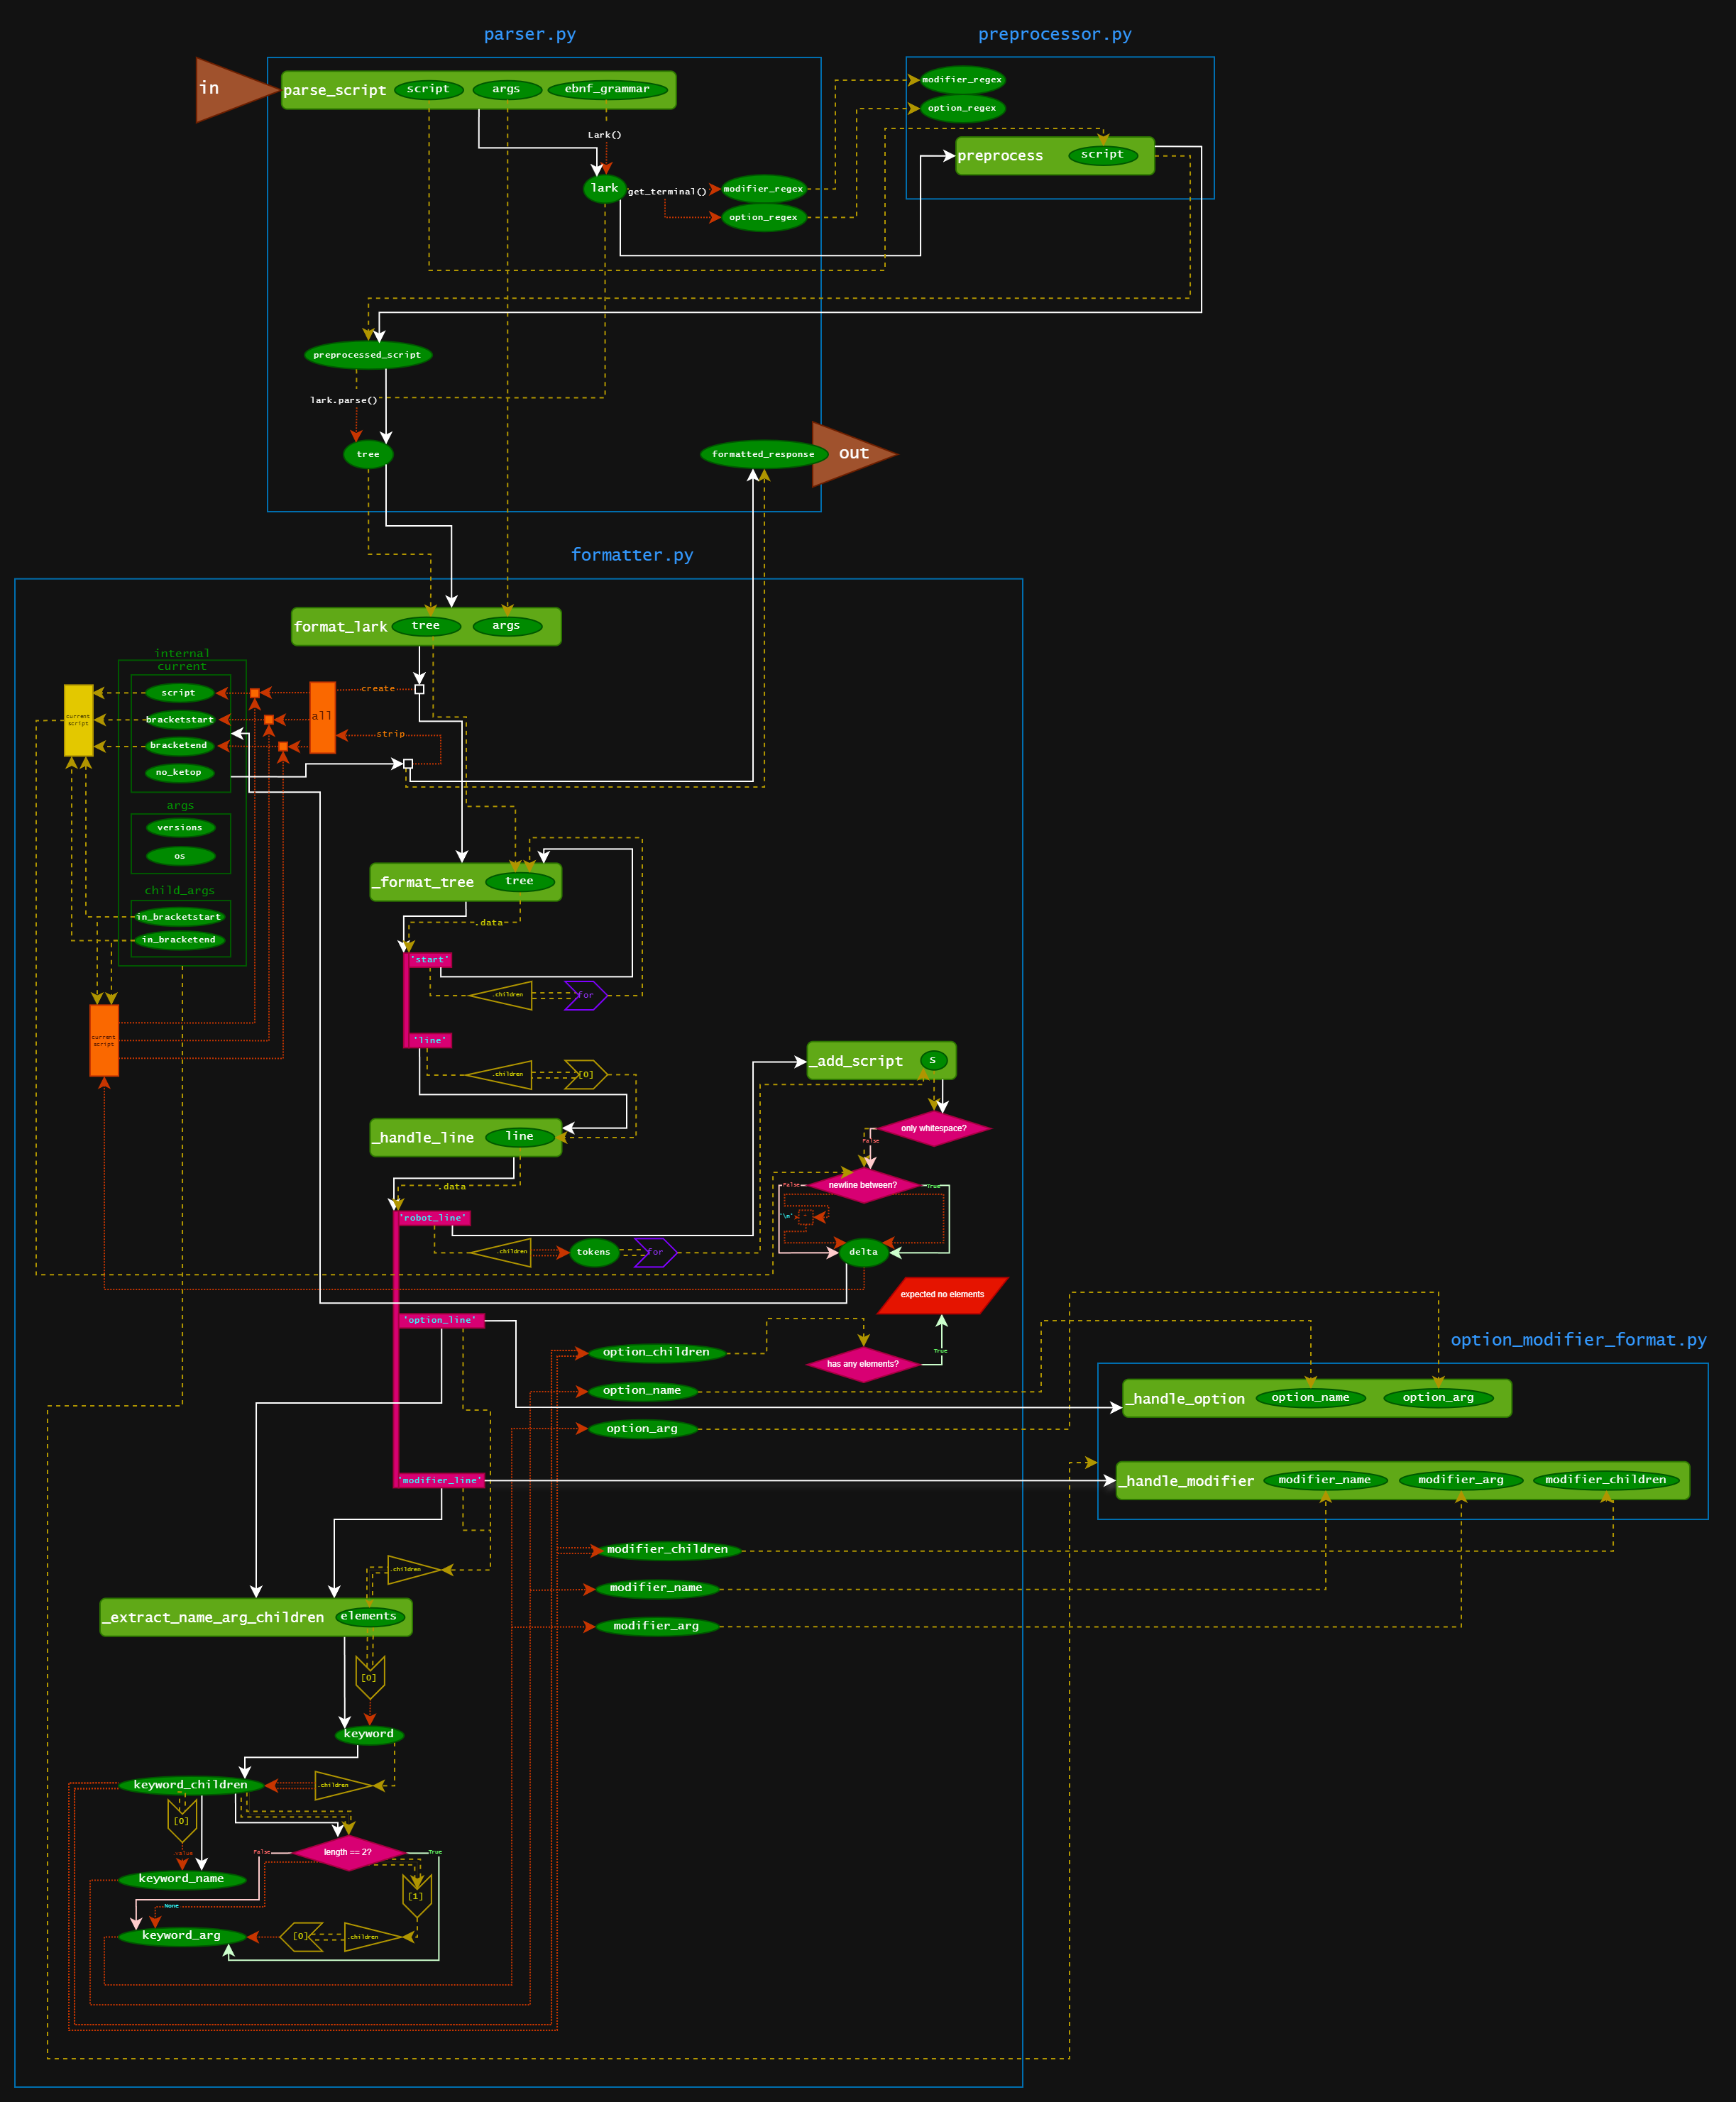
\includegraphics[width=0.35\linewidth]{pics/parser-flowchart/full.png}
        \caption{Downsized flowchart diagram of the parser.}
        \label{fig:parser-flowchart_full}
    \end{subfigure}\hfill
    \begin{subfigure}[b]{\linewidth}
        \centering
        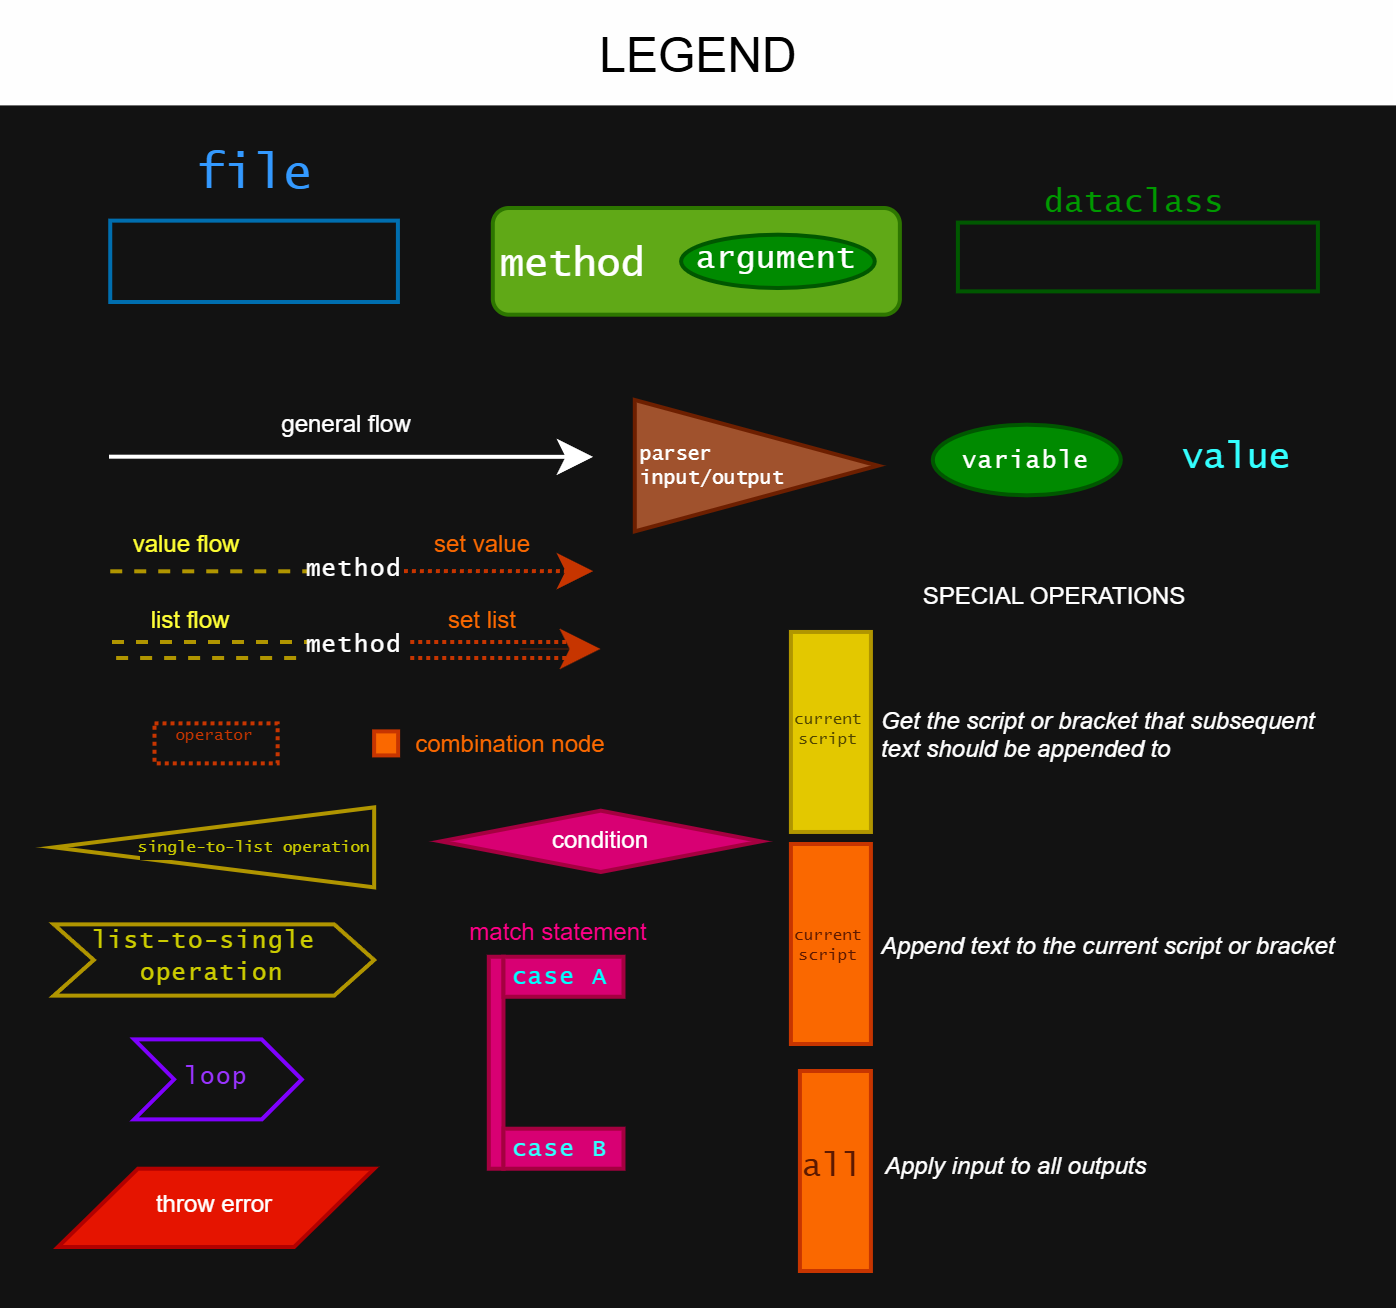
\includegraphics[width=0.6\linewidth]{pics/parser-flowchart/legend.png}
        \caption{Legend of the parser flowchart diagram.}
        \label{fig:parser-flowchart_legend}
    \end{subfigure}
    \caption{Full flowchart diagram of the parser with its legend.}
    \label{fig:parser-flowchart_full_combined}
\end{figure}

It is important to note that while Figure~\ref{fig:parser-flowchart_full} is at a size where it may not be possible to make out details, subsequent sections of this chapter include enlarged variants, as seen in Figures~\ref{fig:parser-flowchart_general_combined},~\ref{fig:parser-flowchart_line-formatting_combined},~\ref{fig:parser-flowchart_line-formatting_location}, and~\ref{fig:parser-flowchart_extract-name-arg-children_combined}.

\section{High-Level Overview}

In a nutshell, the parser takes an input in the form of a script as a string, a few contextual arguments as \verb|FormatterArgs|, and a Lark grammar, which resembles an EBNF grammar, as a string, and outputs a \verb|FormattedResponse|, as is evident by its method header:

\begin{lstlisting}[language=Python, caption={Method header of \texttt{parse\_script}.}, label={lst:method_header_parser_parse_script}]
def parse_script(script:str, args:FormatterArgs, ebnf_grammar:str)->FormattedResponse:
\end{lstlisting}

\subsection{Input: Script}

The script is the the raw Robot script that is to be parsed. Importantly, this input should not already have gone through the preprocessor step mentioned in Chapter~\ref{chap:preprocessor}, as it is done in the function.

\subsection{Input: Arguments}

In the method header, \verb|formatter_args| refers to an instance of the \verb|FormatterArgs| class, which is defined to be the following:

\begin{lstlisting}[language=Python, caption={Class definition of \texttt{FormatterArgs}.}, label={lst:class_definition_parser_formatter_args}]
@dataclass
class FormatterArgs:
    versions:dict[str, str] # label -> version
    os:str|None
\end{lstlisting}

This is used for providing the contextual input, which, in our case, is needed to evaluate the conditions specified in the \verb|@VERSION| and \verb|@OS| modifiers. 

Here, \verb|versions| should be a dictionary object that maps the label of a module to its actual version on the KeTop. In the actual implementation of \verb|@VERSION|, the operation specified in the argument will be checked against the version provided here for the respective module. 

\verb|os| refers to the operating system of the KeTop as a string, or \verb|None| if one is not provided or present (as is generally the case when, for instance, the \verb|no_ketop| flag is set). In the actual implementation of \verb|@OS|, the block body will only be included if the operating system specified in the argument equals the operating system provided here. If no operating system is provided, \verb|@OS| will always discard its block body.

\subsection{Input: Lark grammar}

The Lark grammar, in the method header labeled as \verb|ebnf_grammar|, represents ``a list of rules and terminals that together define a language''\cite{py-module-lark-grammar} as a string. While the Lark library uses its own syntax, it is based on EBNF~\cite{py-module-lark-grammar}.

In our project, the following string, which is a modified form of the our EBNF to abide by Lark's expected syntax, gets used:

\begin{lstlisting}[caption={Our EBNF defined using Lark's syntax.}, label={lst:our_ebnf_lark}]
start: N* (line N*)*

robot_line: /[^(@|\n)].+?(?=\n)/

option_line: "@" option 

modifier_line: "@" modifier ( N )* ( line N* )* "@" "END"

line: modifier_line | option_line | robot_line

modifier: ALLOWED_MODIFIERS arg?
option: ALLOWED_OPTIONS arg?

arg: /[ \t]+[^\n]*/

N: "\n"

%import common.WS_INLINE
%ignore WS_INLINE

ALLOWED_OPTIONS: "NO_KETOP" 
ALLOWED_MODIFIERS: "VERSION" | "BRACKETSTART" | "BRACKETEND" | "OS" | "PREAMBLE"
\end{lstlisting}

The following is changed in listing \ref{lst:our_ebnf_lark} compared to listing \ref{lst:our_ebnf}:
\begin{itemize}
    \item Grammar definition syntax is changed from \verb|=| to \verb|:| and the seperator character between terminals (\verb|,|) and the end-of-rule character (\verb|;|) are omitted.
    \item Repetition is changed from using curly braces (\verb|{...}|) to an asterisk (\verb|...*|). It is important to note that, while it is not needed for our EBNF, Lark also allows for the definition of \textit{one or more} using a plus sign (\verb|...+|) instead.
    \item Optionals are changed from using square brackets (\verb|[...]|) to \verb|...?|.
    \item \gls{regex} tokens are written using slashes (\verb|/.../|).
    \item Terminals (here \verb|N|, \verb|ALLOWED_OPTIONS|, and \verb|ALLOWED_MODIFIERS|) are defined using uppercase.
    \item The verbose definition of the \verb|block body| rule is omitted, and it is instead defined directly within a \verb|modifier_line|.
    \item Inline whitespace is being explicitely ignored using \verb|%import common.WS_INLINE| and \verb|%ignore common.WS_INLINE|. % it says there's an error here because of the percent sign, but it seems to work fine
\end{itemize}

It is important to mention that, while it might be possible to provide a different grammar, it is very likely to cause issues given the strict adherence of our parser to the above grammar. 

\subsection{Output: FormattedResponse}

As long as no exceptions occur, the output of the \verb|parse_script| function will be an instance of the \verb|FormattedResponse| class, which is defined to be the following:

\begin{lstlisting}[language=Python, caption={Class definition of \texttt{FormattedResponse}.}, label={lst:class_definition_parser_formatted_response}]
@dataclass
class FormattedResponse:
    script:str
    preamble_dict:dict[int, str]
    bracketstart:str
    bracketend:str
    no_ketop:bool 
\end{lstlisting}

Here, \verb|script| refers to the general part of the script that is not part of a \textit{bracket}. The term \textit{bracket} refers to a block body of either \verb|@PREAMBLE|, \verb|@BRACKETSTART|, or \verb|@BRACKETEND|. If a Robot script with no Script Assembler keywords is provided as input, aside from possible minor whitespace changes, it will be returned without edit in \verb|script|. 

\verb|preamble_dict| is a dictionary that maps the block bodies of \verb|@PREAMBLE| modifiers to the number given by their respective arguments. 

\verb|bracketstart| and \verb|bracketend| contain the block bodies of \verb|@BRACKETSTART| and\\
\verb|@BRACKETEND| respectively. 

\verb|no_ketop| represents whether or not the \verb|no_ketop| flag is enabled; i.e.\ whether or not the input script contains the \verb|@NO_KETOP| modifier.

\section{Lark}

Lark is a parsing library for Python which can parse any context-free grammar to an object known as a \textit{tree}~\cite{py-module-lark}.

After preprocessing, the Script Assembler uses the input script on Lark's \verb|parse| method to get a \verb|Tree| object which, amongst others, includes two important properties: \verb|data| and \verb|children|.

A \verb|Tree| object represents a rule with a name, for example, the outermost rule of a parsed script being \verb|"start"|, alongside, if present, its children, which, in the example of \verb|"start"| are \verb|"line"|s. A \textit{child} is commonly a \verb|Tree| as well, however it may also be a \verb|Token|~\cite{py-module-lark-api}.

According to Lark's official \gls{api} reference, a \verb|Token| is described as the following:

\begin{quote}
``A string with meta-information, that is produced by the lexer. When parsing text, the resulting chunks of the input that haven't been discarded, will end up in the tree as Token instances. The Token class inherits from Python's \verb|str|, so normal string comparisons and operations will work as expected.''\cite{py-module-lark-api}
\end{quote}

In our parser, we mainly work with \verb|Tree|s to differentiate between lines and keywords, and \verb|Token|s for the contents of robot lines and keyword arguments. 

\section{General Procedure}

The \verb|parse_script| starts by creating an instance of the \verb|Lark| class using the provided grammar. Using Lark's \verb|get_terminal| function, the allowed modifiers and options as specified in the grammar are fetched and, together with the input script, passed to the preprocessor. 

Afterwards, using Lark's \verb|parse| method, the preprocessed script is then converted to a \verb|Tree| object. This is passed to the \verb|format_lark| function, which utilizes the provided \verb|FormatterArgs| to turn it into a \verb|FormattedResponse|, which is then returned. 

Figure~\ref{fig:parser-flowchart_general_combined} highlights this procedure.

\begin{figure}[H]
    \centering
    
    \begin{subfigure}[b]{\linewidth}
        \centering
        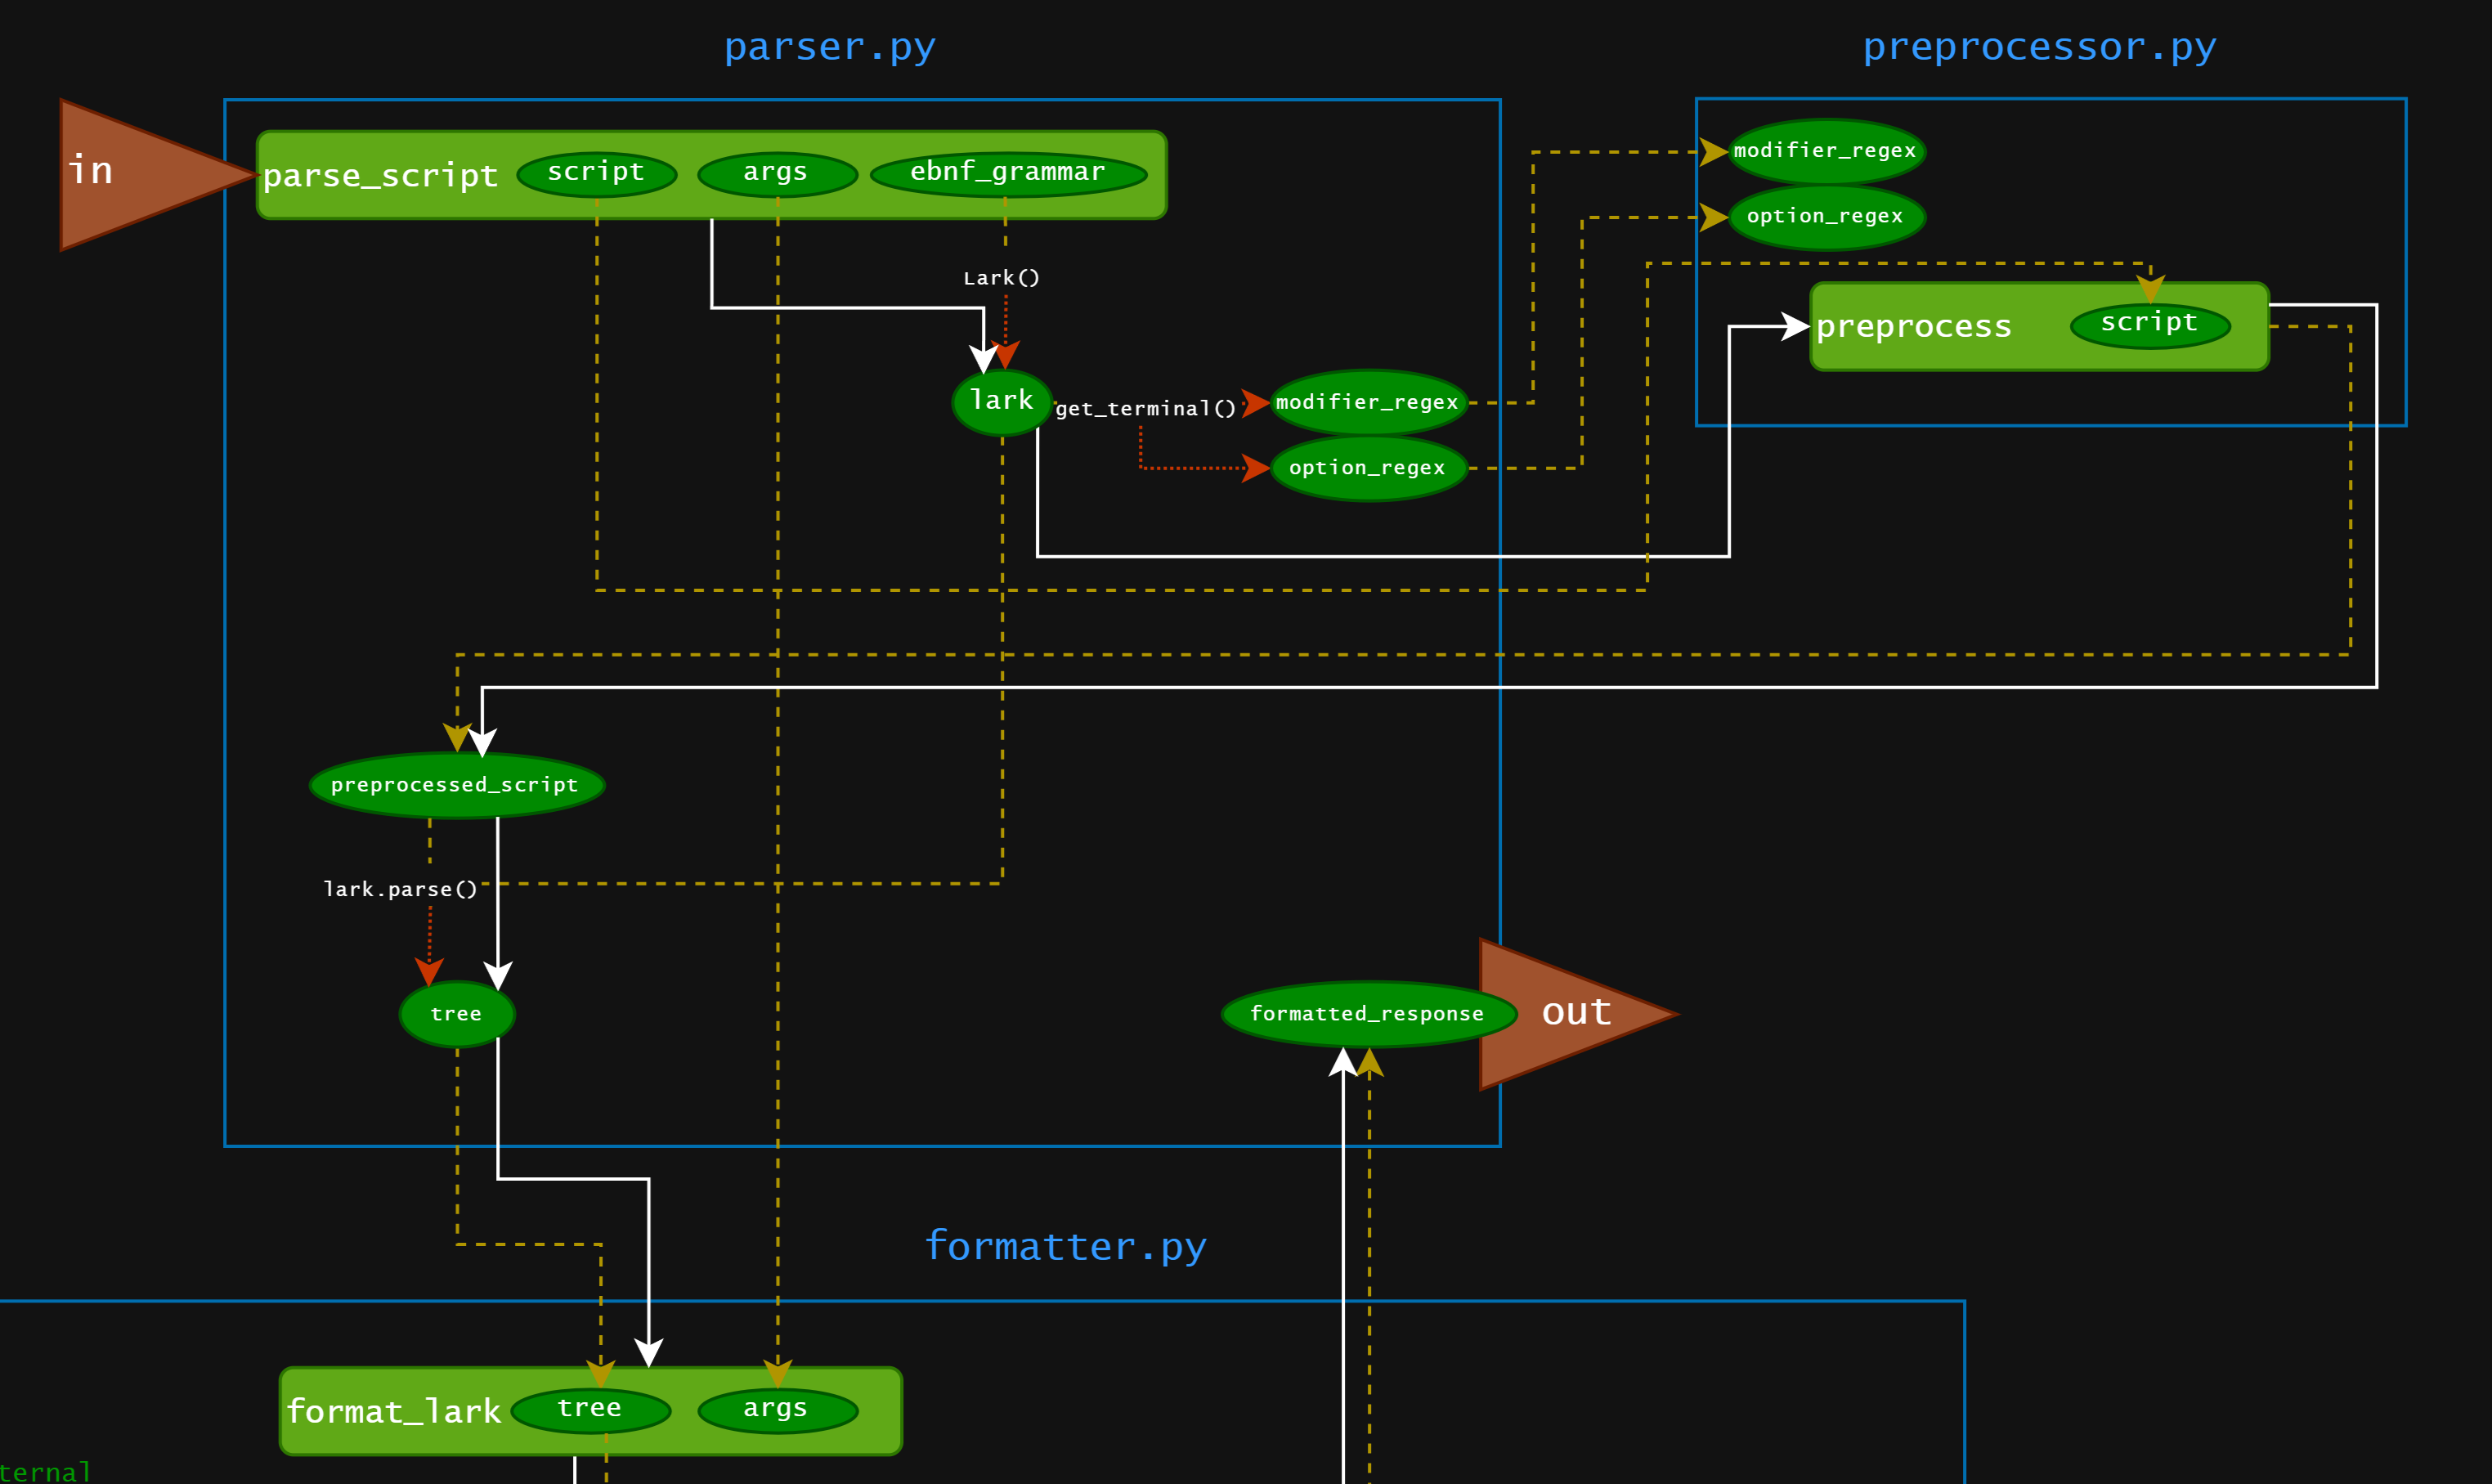
\includegraphics[width=\linewidth]{pics/parser-flowchart/general.png}
        \caption{The detailed part of the parser's flowchart diagram which illustrates the general procedure.}
        \label{fig:parser-flowchart_general}
    \end{subfigure}

    \vspace{6pt}

    \begin{subfigure}[b]{\linewidth}
        \centering
        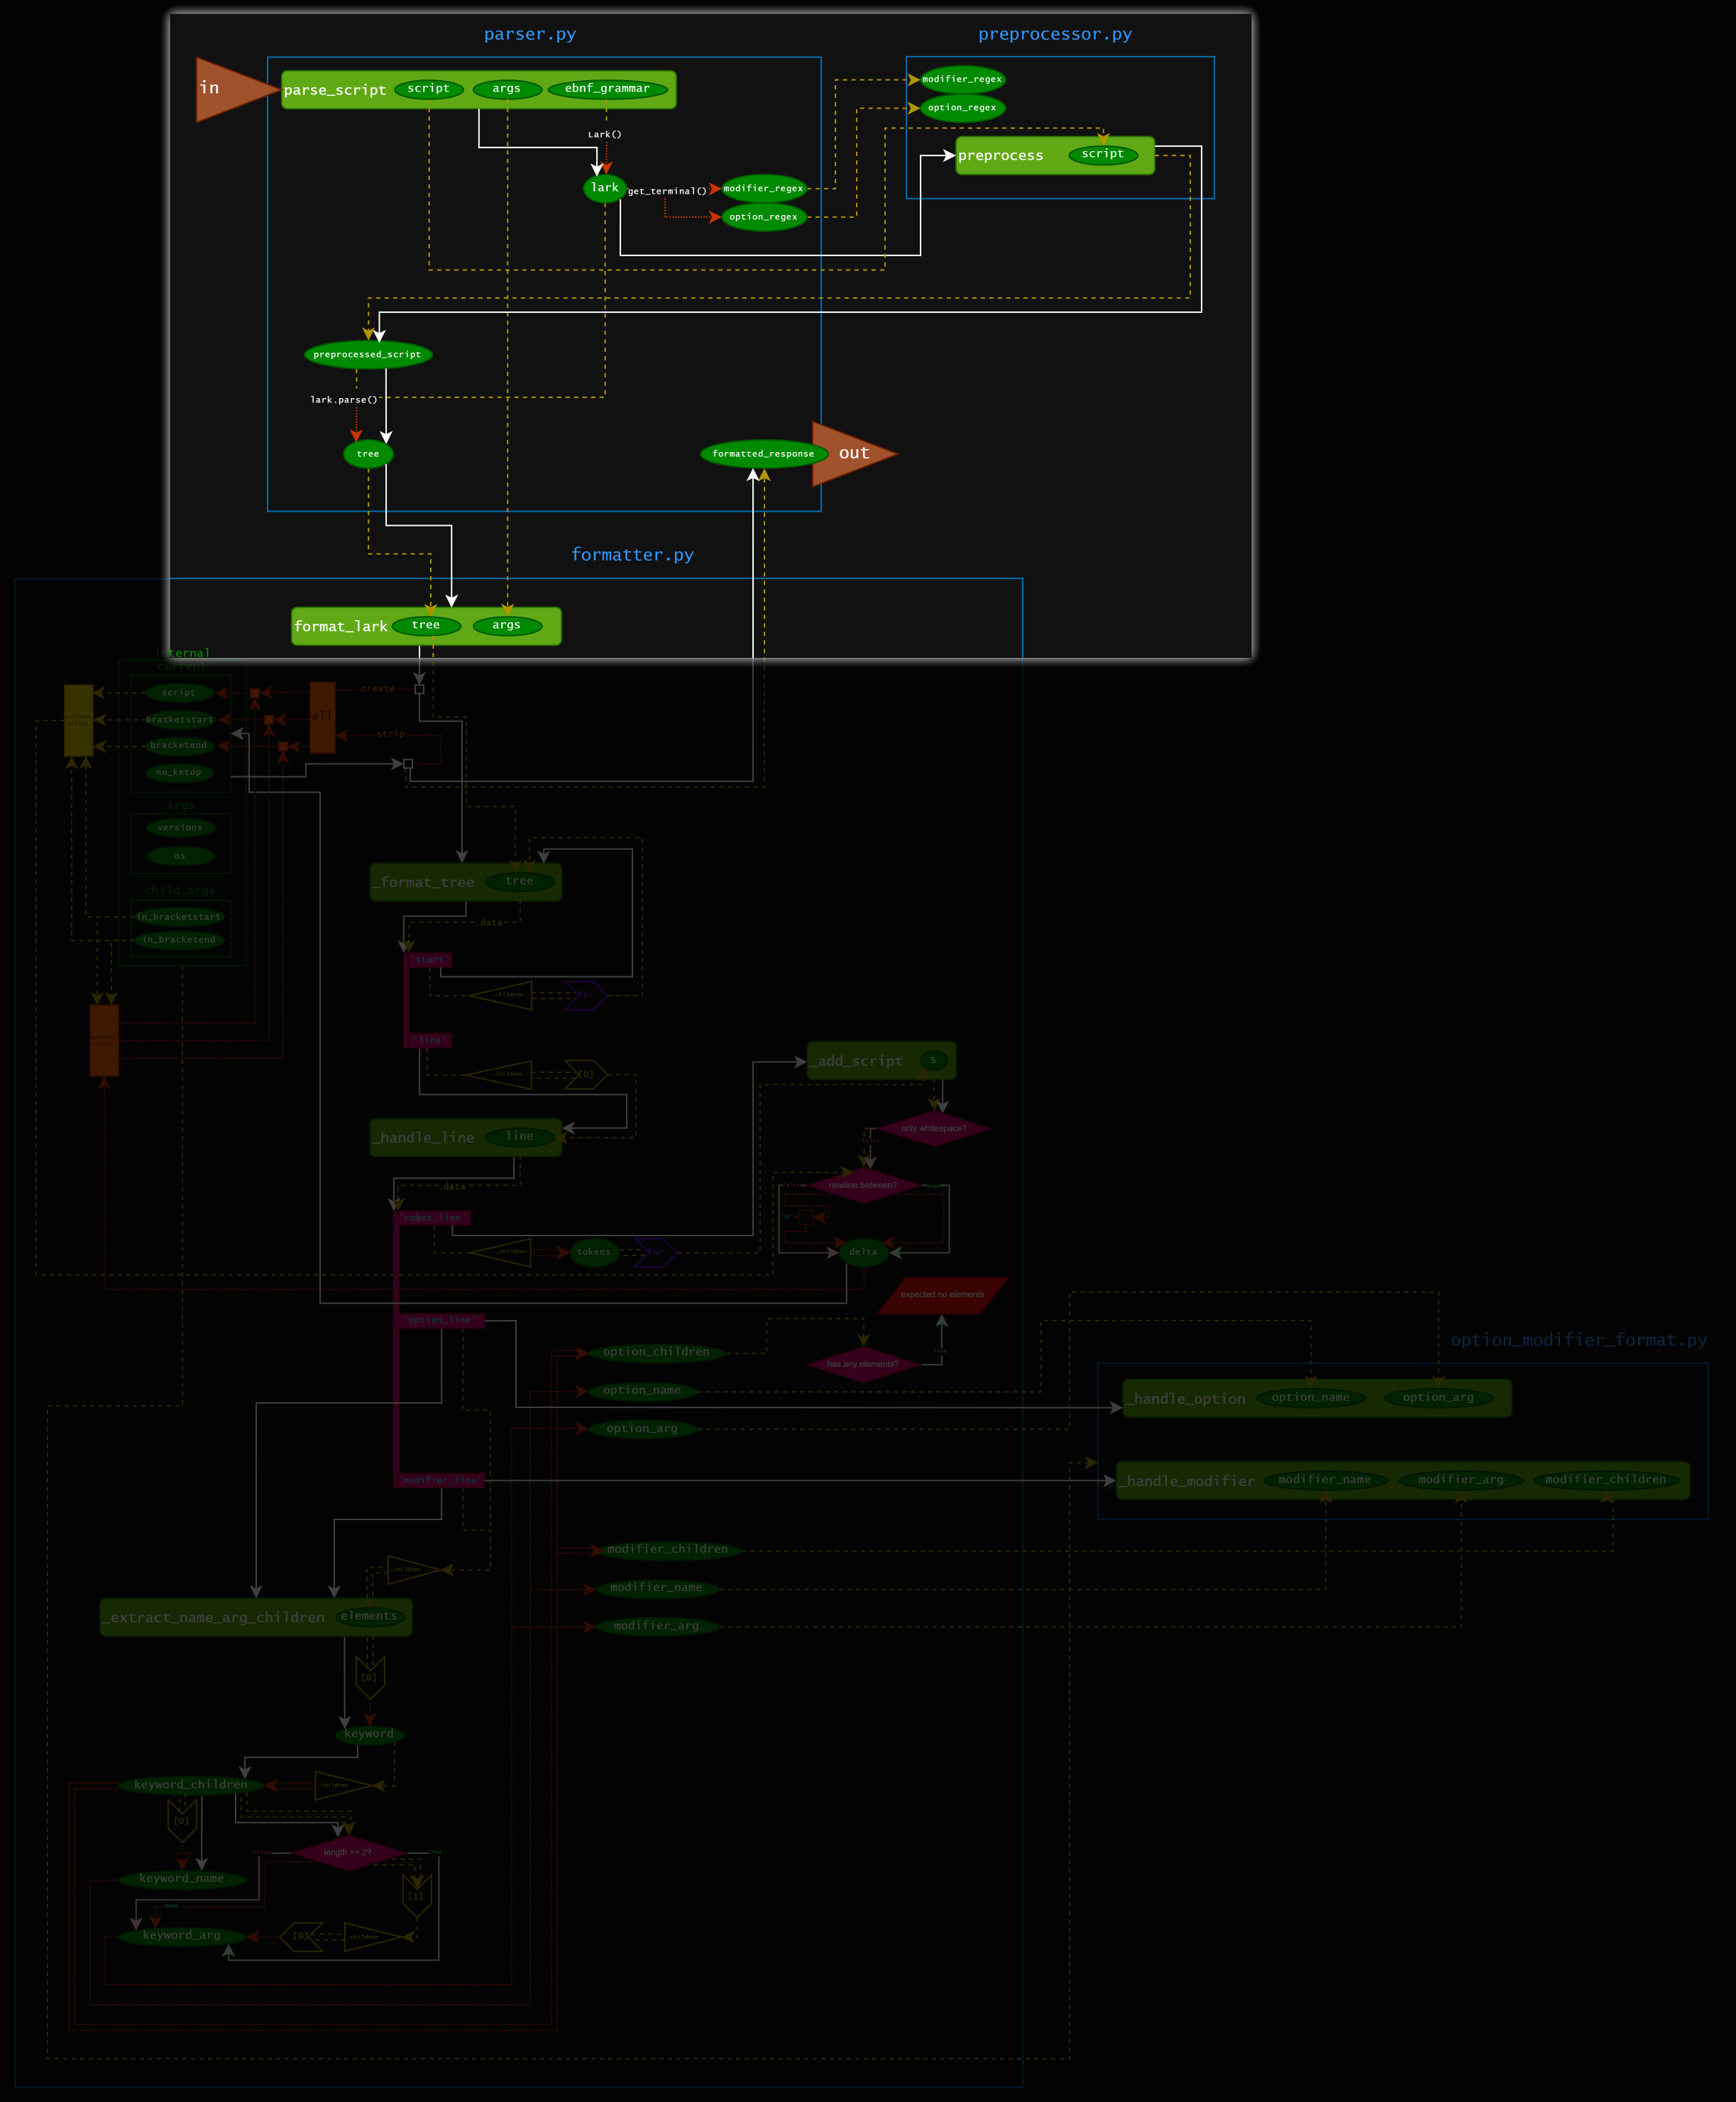
\includegraphics[width=0.35\linewidth]{pics/parser-flowchart/general_location.png}
        \caption{The location of the detailed inset within the full flowchart as seen in Figure~\ref{fig:parser-flowchart_full}.}
        \label{fig:parser-flowchart_general_location}
    \end{subfigure}

    \caption{The part of the flowchart diagram from Figure~\ref{fig:parser-flowchart_full_combined} that details the general procedure of the parser.}
    \label{fig:parser-flowchart_general_combined}
\end{figure}

\section{Formatter}

After a script has been preprocessed and parsed by Lark, the \verb|Tree| object is given to the method from the \verb|Formatter| class with the following header:

\begin{lstlisting}[language=Python, caption={Method header of \texttt{format_lark}.}, label={lst:method_header_parser_format_lark}]
def format_lark(self, tree:Tree, args:FormatterArgs)->FormattedResponse:
\end{lstlisting}

The \verb|Formatter| class recursively parses the \verb|tree|'s children to eventually return a \verb|FormattedResponse|. 

\subsection{FormatterInternal}

The formatter keeps track of the current state of the parsing using an internal property named \verb|current| that is of type \verb|FormatterInternal| which is defined as the following:

\begin{lstlisting}[language=Python, caption={Class definition of \texttt{FormatterInternal}.}, label={lst:class_definition_parser_formatter_internal}]
@dataclass
class FormatterInternal:
    current:FormattedResponse
    args:FormatterArgs
    child_args:ChildArgs
\end{lstlisting}

This \verb|FormatterInternal| instance is unique per formatting operation and it is passed to any functions that need the context of the formatter.\ \verb|args| represents the instance of \verb|FormatterArgs| that was provided to the parser that includes information on versions and operating system. 

When the \verb|format_lark| function finishes without error, it returns the \verb|current| property of the \verb|FormatterInternal| instance it uses to keep track. 

\subsection{ChildArgs}

\verb|child_args| is used for modifiers and their recursive nature. When a line belonging to the block body of a modifier is handled, it may need to be handled differently depending on factors such as whether or not that line should be part of a bracket. 

When a \verb|modifier_line| is hit, the function handling that modifier may return a new instance of \verb|ChildArgs|. Then, this instance will be used for all lines that belong to the block body of that modifier. 

The \verb|ChildArgs| class is defined to be the following:

\begin{lstlisting}[language=Python, caption={Class definition of \texttt{ChildArgs}.}, label={lst:class_definition_parser_child_args}]
@dataclass
class ChildArgs:
    preamble_index:int = 0
    in_bracketstart:bool = False
    in_bracketend:bool = False
\end{lstlisting}

Here, \verb|preamble_index| represents the index of the preamble bracket that new lines should be appended to. If this variable is set to \verb|0|, it means that the formatter is currently not inside of an \verb|@PREAMBLE| modifier. 

\verb|in_bracketstart| and \verb|in_bracketend| represent whether or not the formatter is currently within a respective \verb|@BRACKETSTART| or \verb|@BRACKETEND| modifier. If either of this is the case, new lines will be appended to the respective \verb|bracketstart| or \verb|bracketend| brackets, respectively.

Here, \verb|preamble_index|, \verb|in_bracketstart|, and \verb|in_bracketend| are mutually exclusive to one another, i.e.\ at most only one of them can be \textit{active} at a time.

\subsection{Line handling}

After the formatter is past the \verb|"start"| entry point of the initial \verb|Tree|, it will run \verb|dle_line| on each line element, which is a function with the following header:

\begin{lstlisting}[language=Python, caption={Method header of \texttt{_handle_line}.}, label={lst:method_definition_parser_handle_line`'}]
def _handle_line(self, line:Tree)->None:
\end{lstlisting}

This function differentiates whether the \verb|line| matches \verb|"robot_line"|, \verb|"option_line"|, or \verb|"modifier_line"| in the following way. Note that all functions listed below will be explained shortly. 

\begin{itemize}
    \item For \verb|"robot_line"|: Since Robot lines are made of, for the purposes of the parser, arbitrary text, they can be added to the output as-is using the \verb|_add_script| function.
    \item For \verb|"option_line"|: The function \verb|OptionModifierFormat.handle_option| is called with the current \verb|FormatterInternal|, the option's name (e.g.\ \verb|"NO_KETOP"|), and, if present, the argument string.
    \item For \verb|"modifier_line"|: The function \verb|OptionModifierFormat.handle_modifier| is called with the current \verb|FormatterInternal|, the modifier's name (e.g.\ \verb|"VERSION"|), if present, the argument string (i.e.\ \verb|BIOS > 1.0.0|), and its children. The children represent the modifier line's block body. Then, the output of this function is given to the \verb|_format_children| function for further processing.
\end{itemize}

\verb|_add_script| adds an input string to the output script or respective bracket. This is the function that appends text (Robot lines) to the final \verb|FormattedResponse|. Where exactly the text gets appended to depends on the state of the current \verb|child_args|. If \verb|child_args| specifies that the formatter is currently within a bracket, it will be appended to \verb|bracketstart|, \verb|bracketend|, or the given index of \verb|preamble_dict|, respectively; otherwise, it will be appended to \verb|script|.

\verb|OptionModifierFormat.handle_option| is part of a seperate class to handle the specific option and, in turn, alter flags of the \verb|current| (\verb|FormattedResponse|) provided in the \verb|FormatterInternal| instance. 

\verb|OptionModifierFormat.handle_modifier| is part of a separate class to handle the specific modifier. Unlike \verb|OptionModifierFormat.handle_option|, this function has return values: firstly, its children (which, as stated above, represent the block body) and the new instance of \verb|ChildArgs| to be used as context information for the lines in its block body. 

\verb|_format_children| sets the formatter's current \verb|ChildArgs| to the instance given as parameter, runs \verb|_handle_line| on each element of the provided list of \verb|Tree|s, and then changes the formatter's current \verb|ChildArgs| value back to what it was at the beginning of this function call. This way, a modifier's \verb|ChildArgs| only gets used for its children (block body). If a modifier does not need to pass custom \verb|ChildArgs| to its children, it may return the \verb|ChildArgs| of \verb|current| (\verb|FormatterInternal|), as opposed to a new instance. 

Figures~\ref{fig:parser-flowchart_line-formatting_combined} and~\ref{fig:parser-flowchart_line-formatting_location} highlight the precise procedure to recursively handle each line.

% Ensure floats before are flushed, then place figures at the top
\FloatBarrier
% Combine the two detailed images into one figure and put the location image separately
\begin{figure}[t!]
    \centering
    \begin{subfigure}[b]{\linewidth}
        \centering
        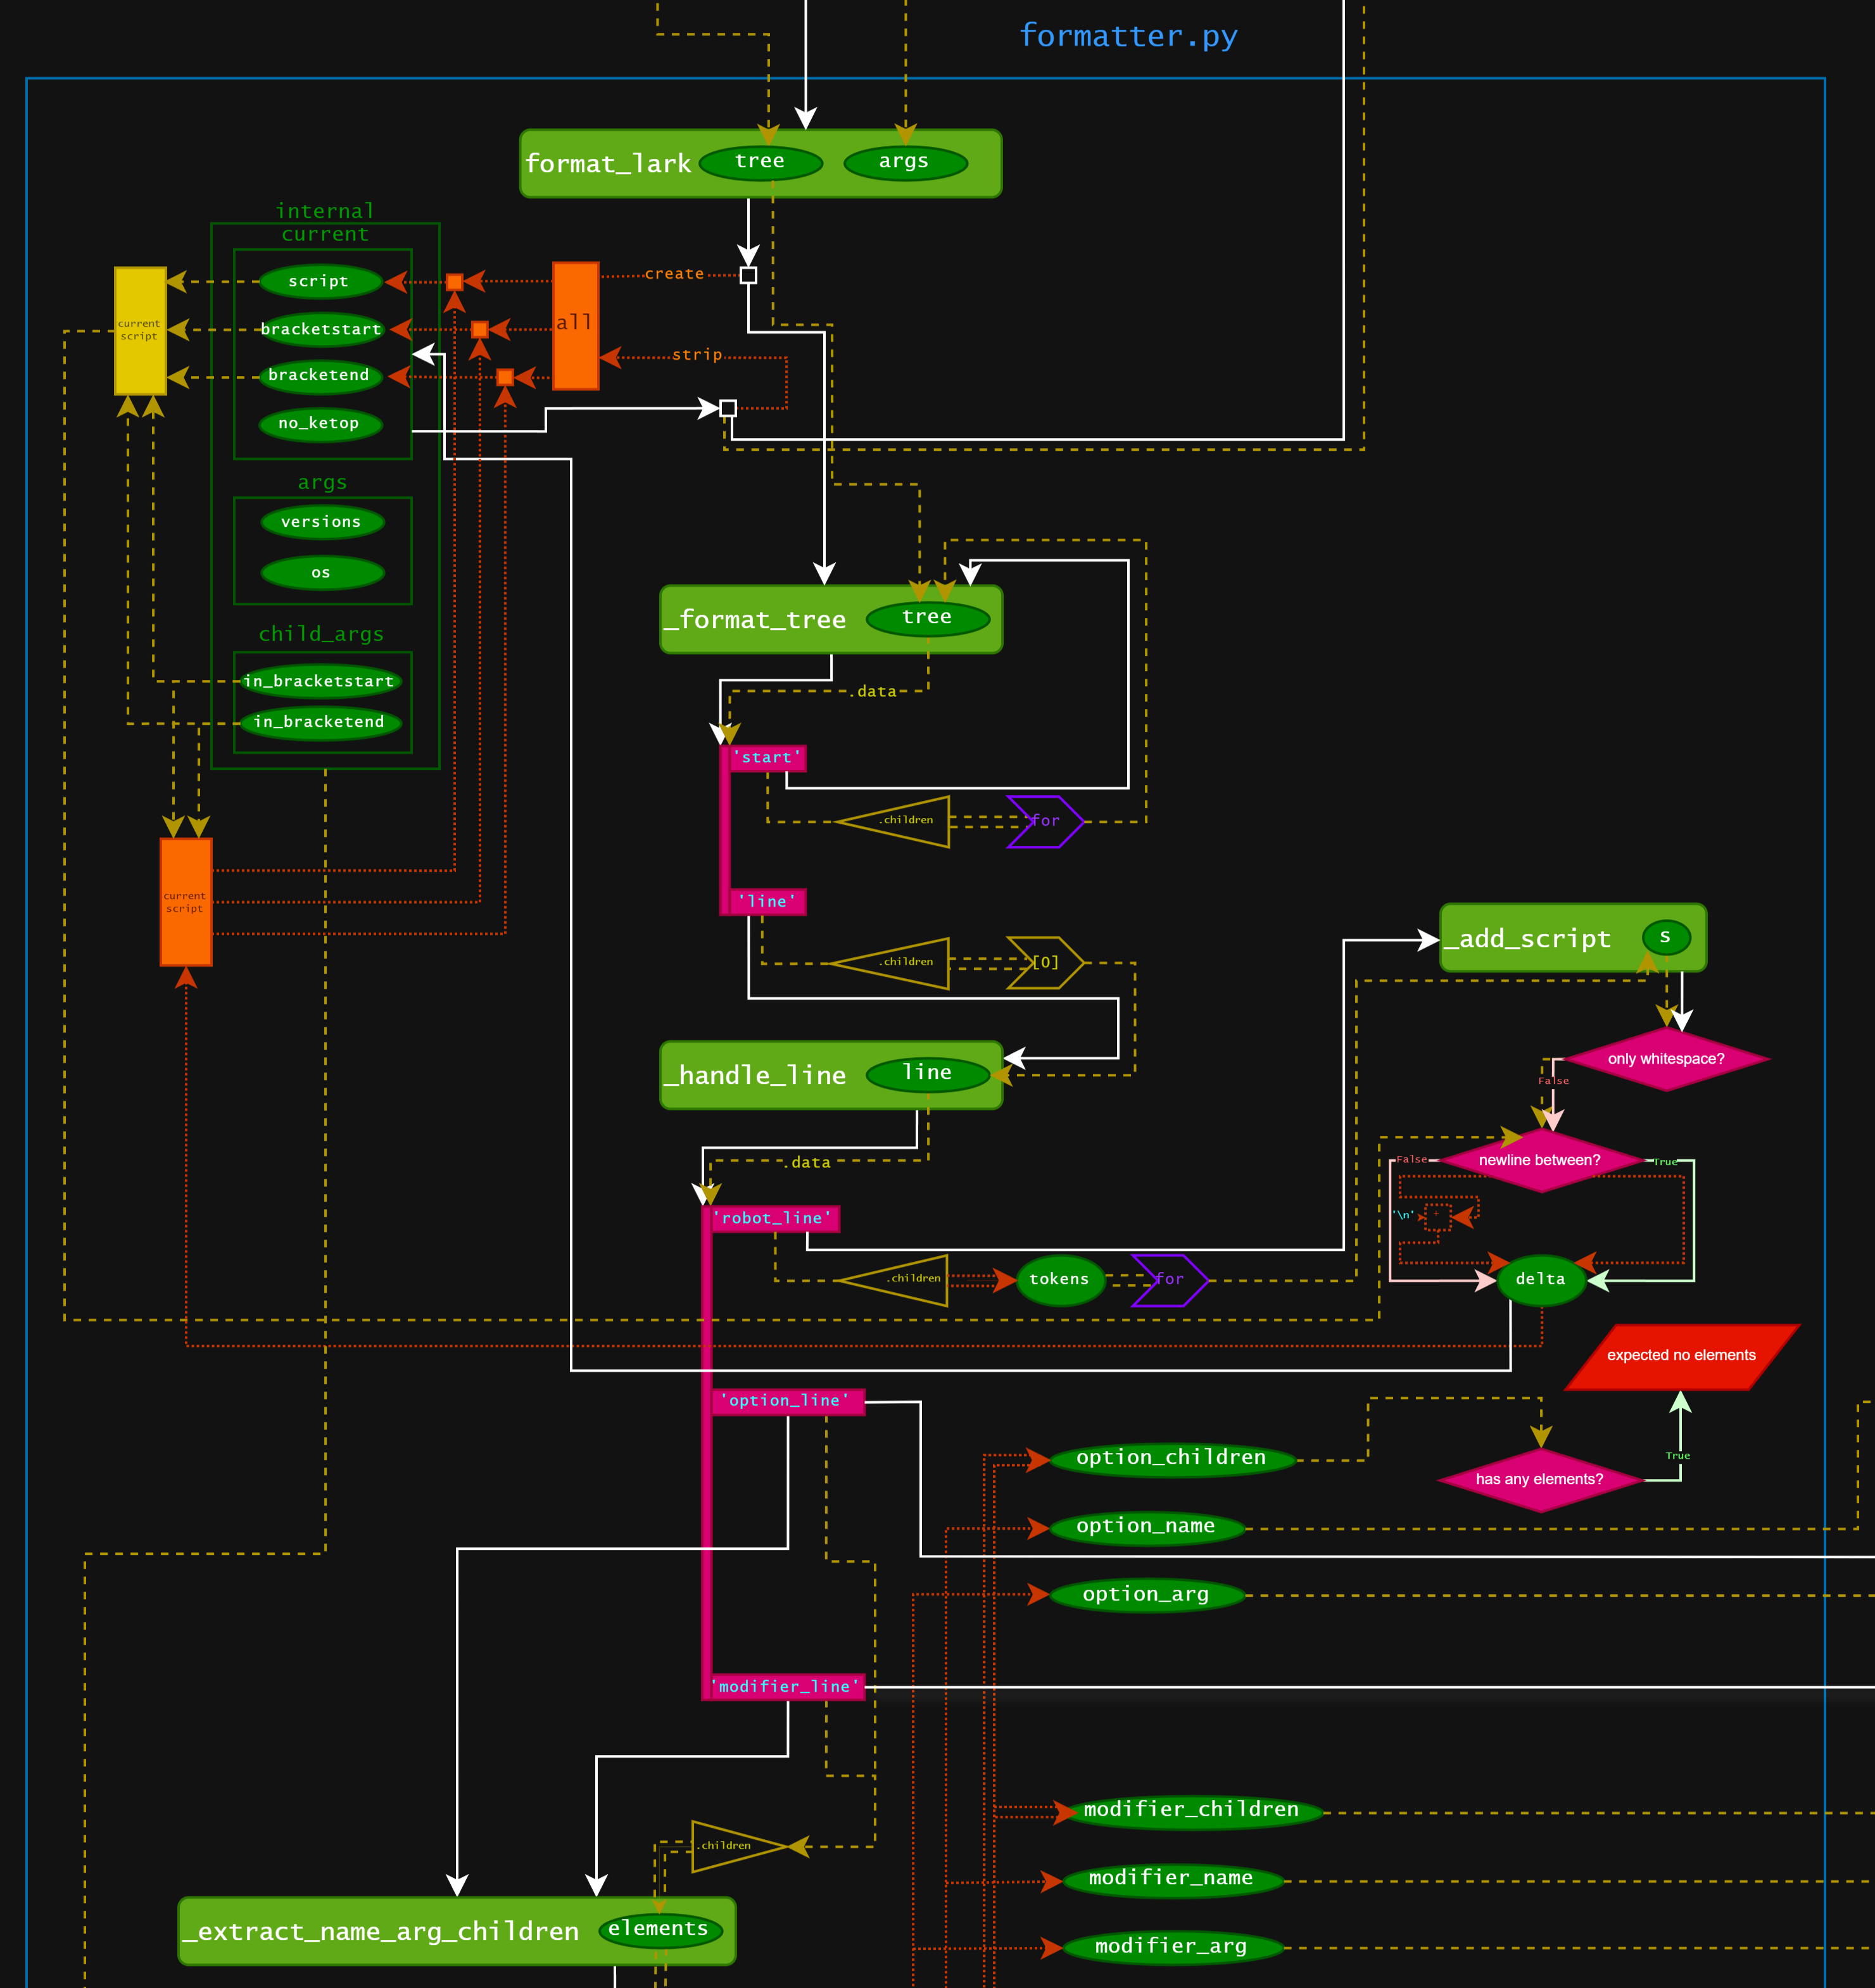
\includegraphics[width=\linewidth]{pics/parser-flowchart/line-formatting-1.png}
        \caption{The detailed part of the parser's flowchart diagram which illustrates how the main part of the formatter recursively handles lines.}
        \label{fig:parser-flowchart_line-formatting-1}
    \end{subfigure}

    \vspace{6pt}

    \begin{subfigure}[b]{\linewidth}
        \centering
        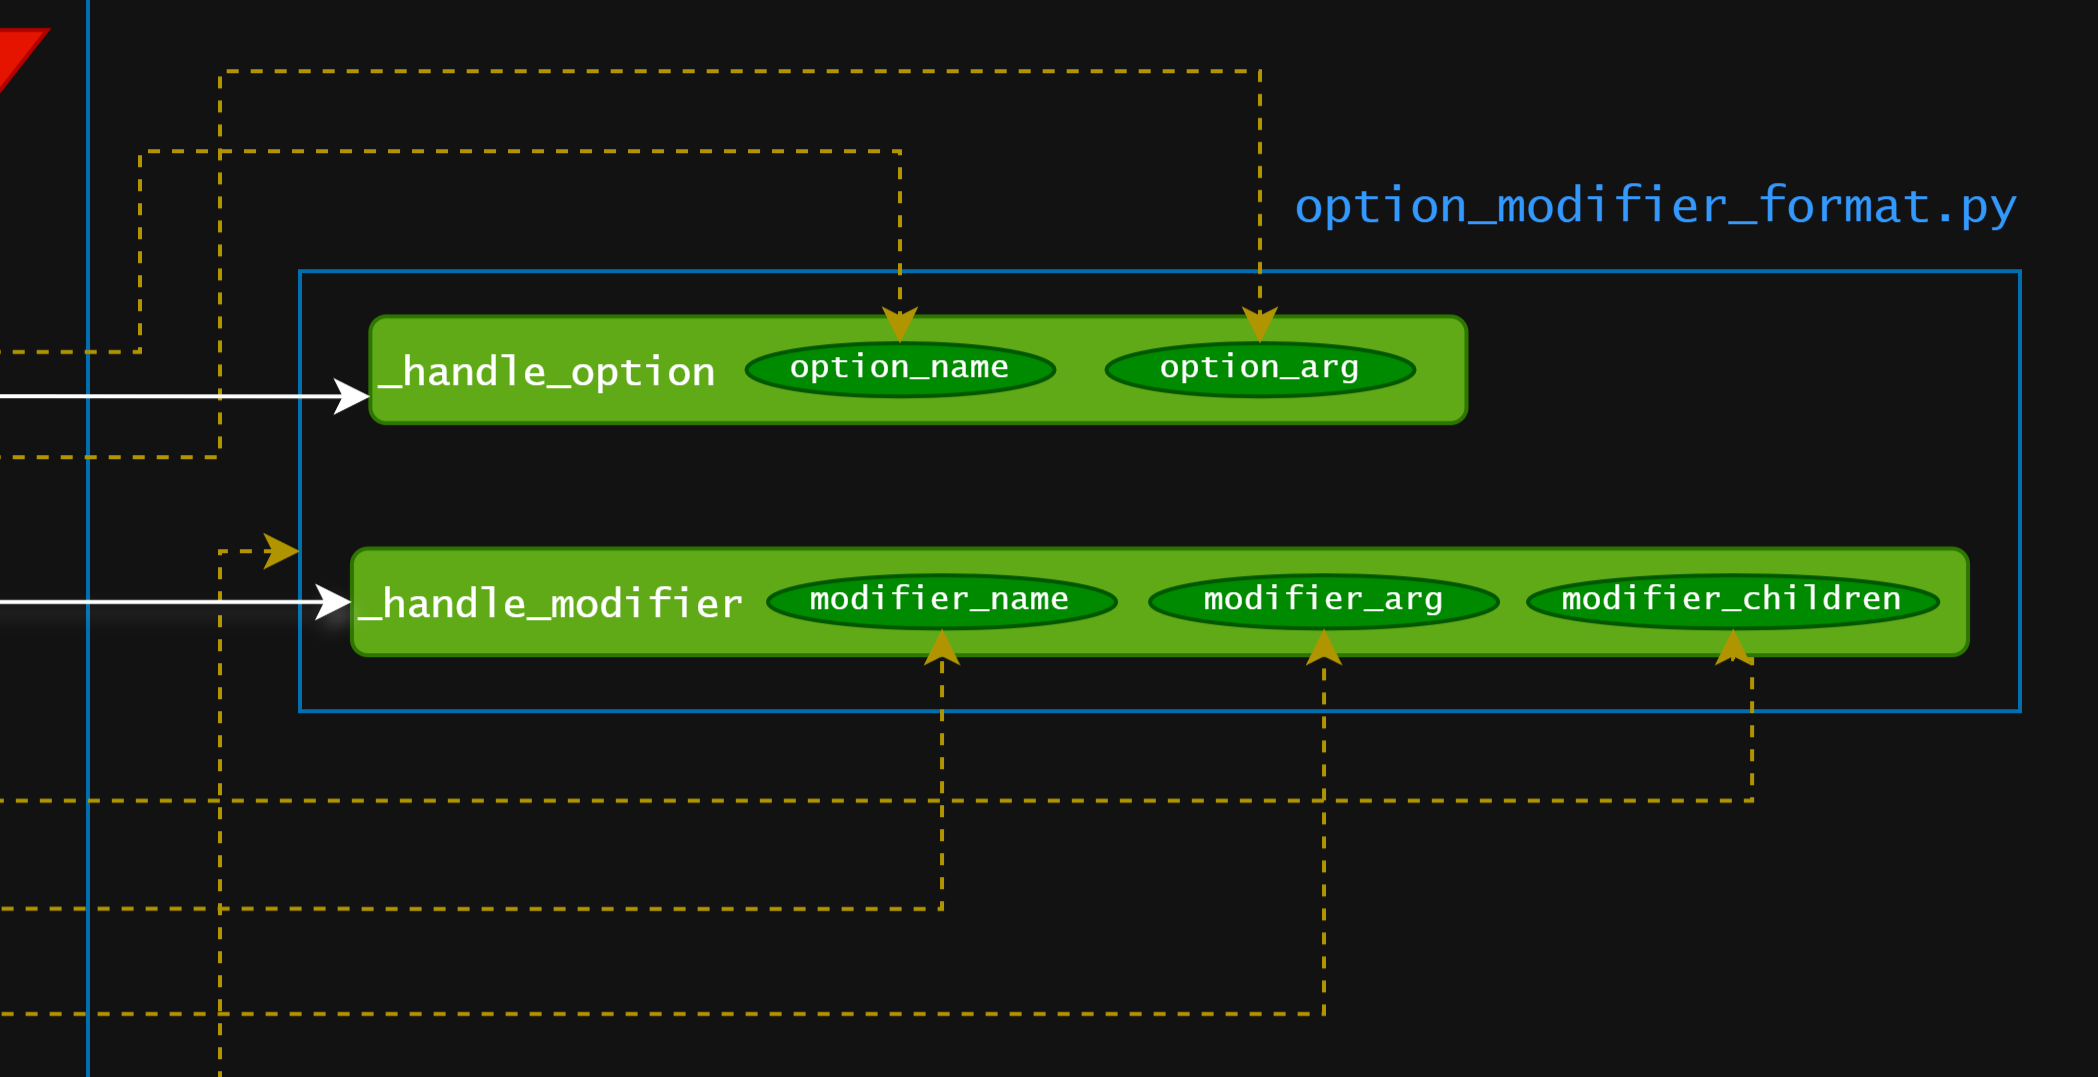
\includegraphics[width=0.7\linewidth]{pics/parser-flowchart/line-formatting-2.png}
        \caption{The detailed part of the parser's flowchart diagram which shows how arguments are passed to Option/Modifier Format.}
        \label{fig:parser-flowchart_line-formatting-2}
    \end{subfigure}

    \caption{Detailed insets for the parser flowchart shown in Figure~\ref{fig:parser-flowchart_full_combined}.}
    \label{fig:parser-flowchart_line-formatting_combined}
\end{figure}

\begin{figure}[t!]
    \centering
    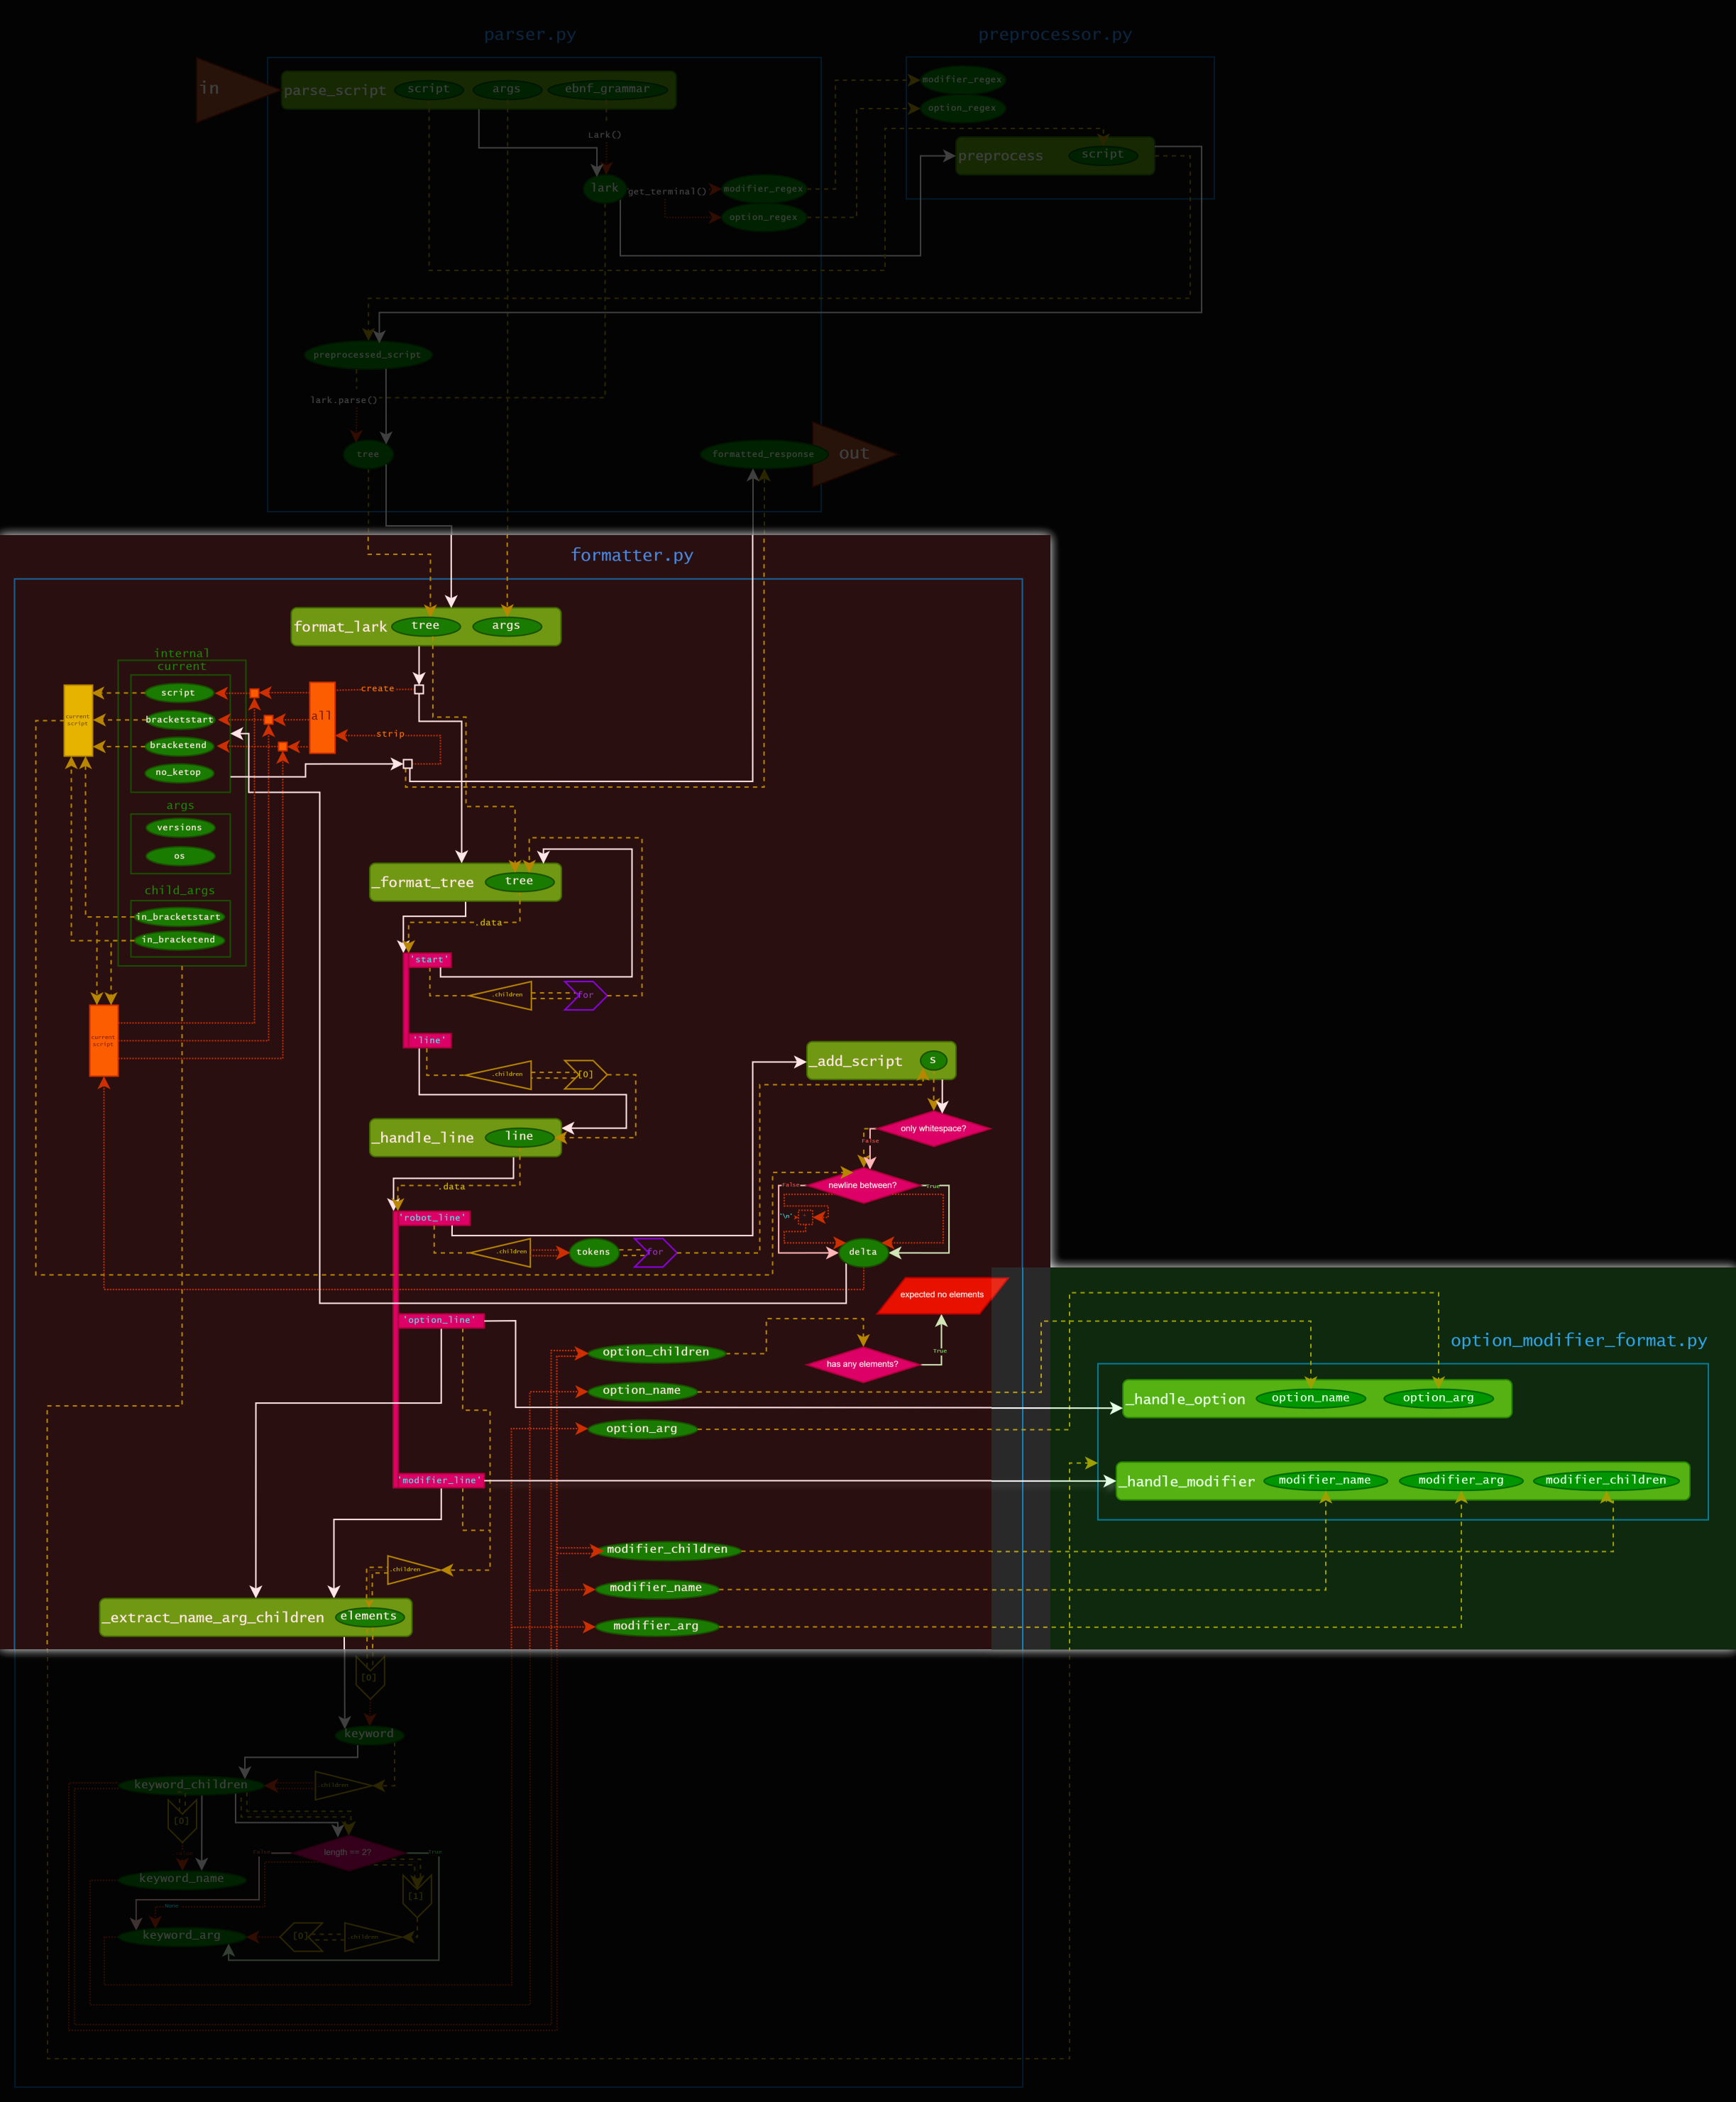
\includegraphics[width=0.45\linewidth]{pics/parser-flowchart/line-formatting_location.png}
    \caption{Location of the detailed insets from Figure~\ref{fig:parser-flowchart_line-formatting_combined} within the full flowchart (Figure~\ref{fig:parser-flowchart_full}).}
    \label{fig:parser-flowchart_line-formatting_location}
\end{figure}

\clearpage

\section{Extracting name, arg, children}

A keyword's name, its argument if present, and its children (block body) get extracted from the \verb|_extract_name_arg_children| function. In the case of an option, the expected amount of children is zero. 

In both cases however, the \verb|children| of the line get passed to this function. Assuming the input to be in the correct general format, the following can be said about the values of the elements of this list, which will be referred to as \verb|elements|:

\begin{itemize}
    \item \verb|elements[0]|: This represents the keyword as option or modifier.\\ 
    Its \verb|$.data| is either \verb|"option"| or \verb|"modifier"|.
    \item \verb|elements[0].children|: This list either contains one or two elements.
    \item \verb|elements[0].children[0]|: This element is a \verb|Token| and its \verb|$.value| represents the name of the keyword (e.g.\ \verb|"VERSION"|). 
    \item \verb|elements[0].children[1]|: If present (i.e.\ if \verb|elements[0].children| contains two elements), its \verb|$.children[0].value| represents the argument. Otherwise, there is no argument. 
    \item \verb|elements[1:]|: The rest of the \verb|elements| list, i.e.\ everything but the first element, is considered the children (block body) of the modifier.
\end{itemize}

Here, \verb|$| is used as a placeholder for the respective variable from before the colon of each bullet point.

Figure~\ref{fig:parser-flowchart_extract-name-arg-children_combined} highlights this procedure.

\begin{figure}[H]
    \centering
    
    \begin{subfigure}[b]{\linewidth}
        \centering
        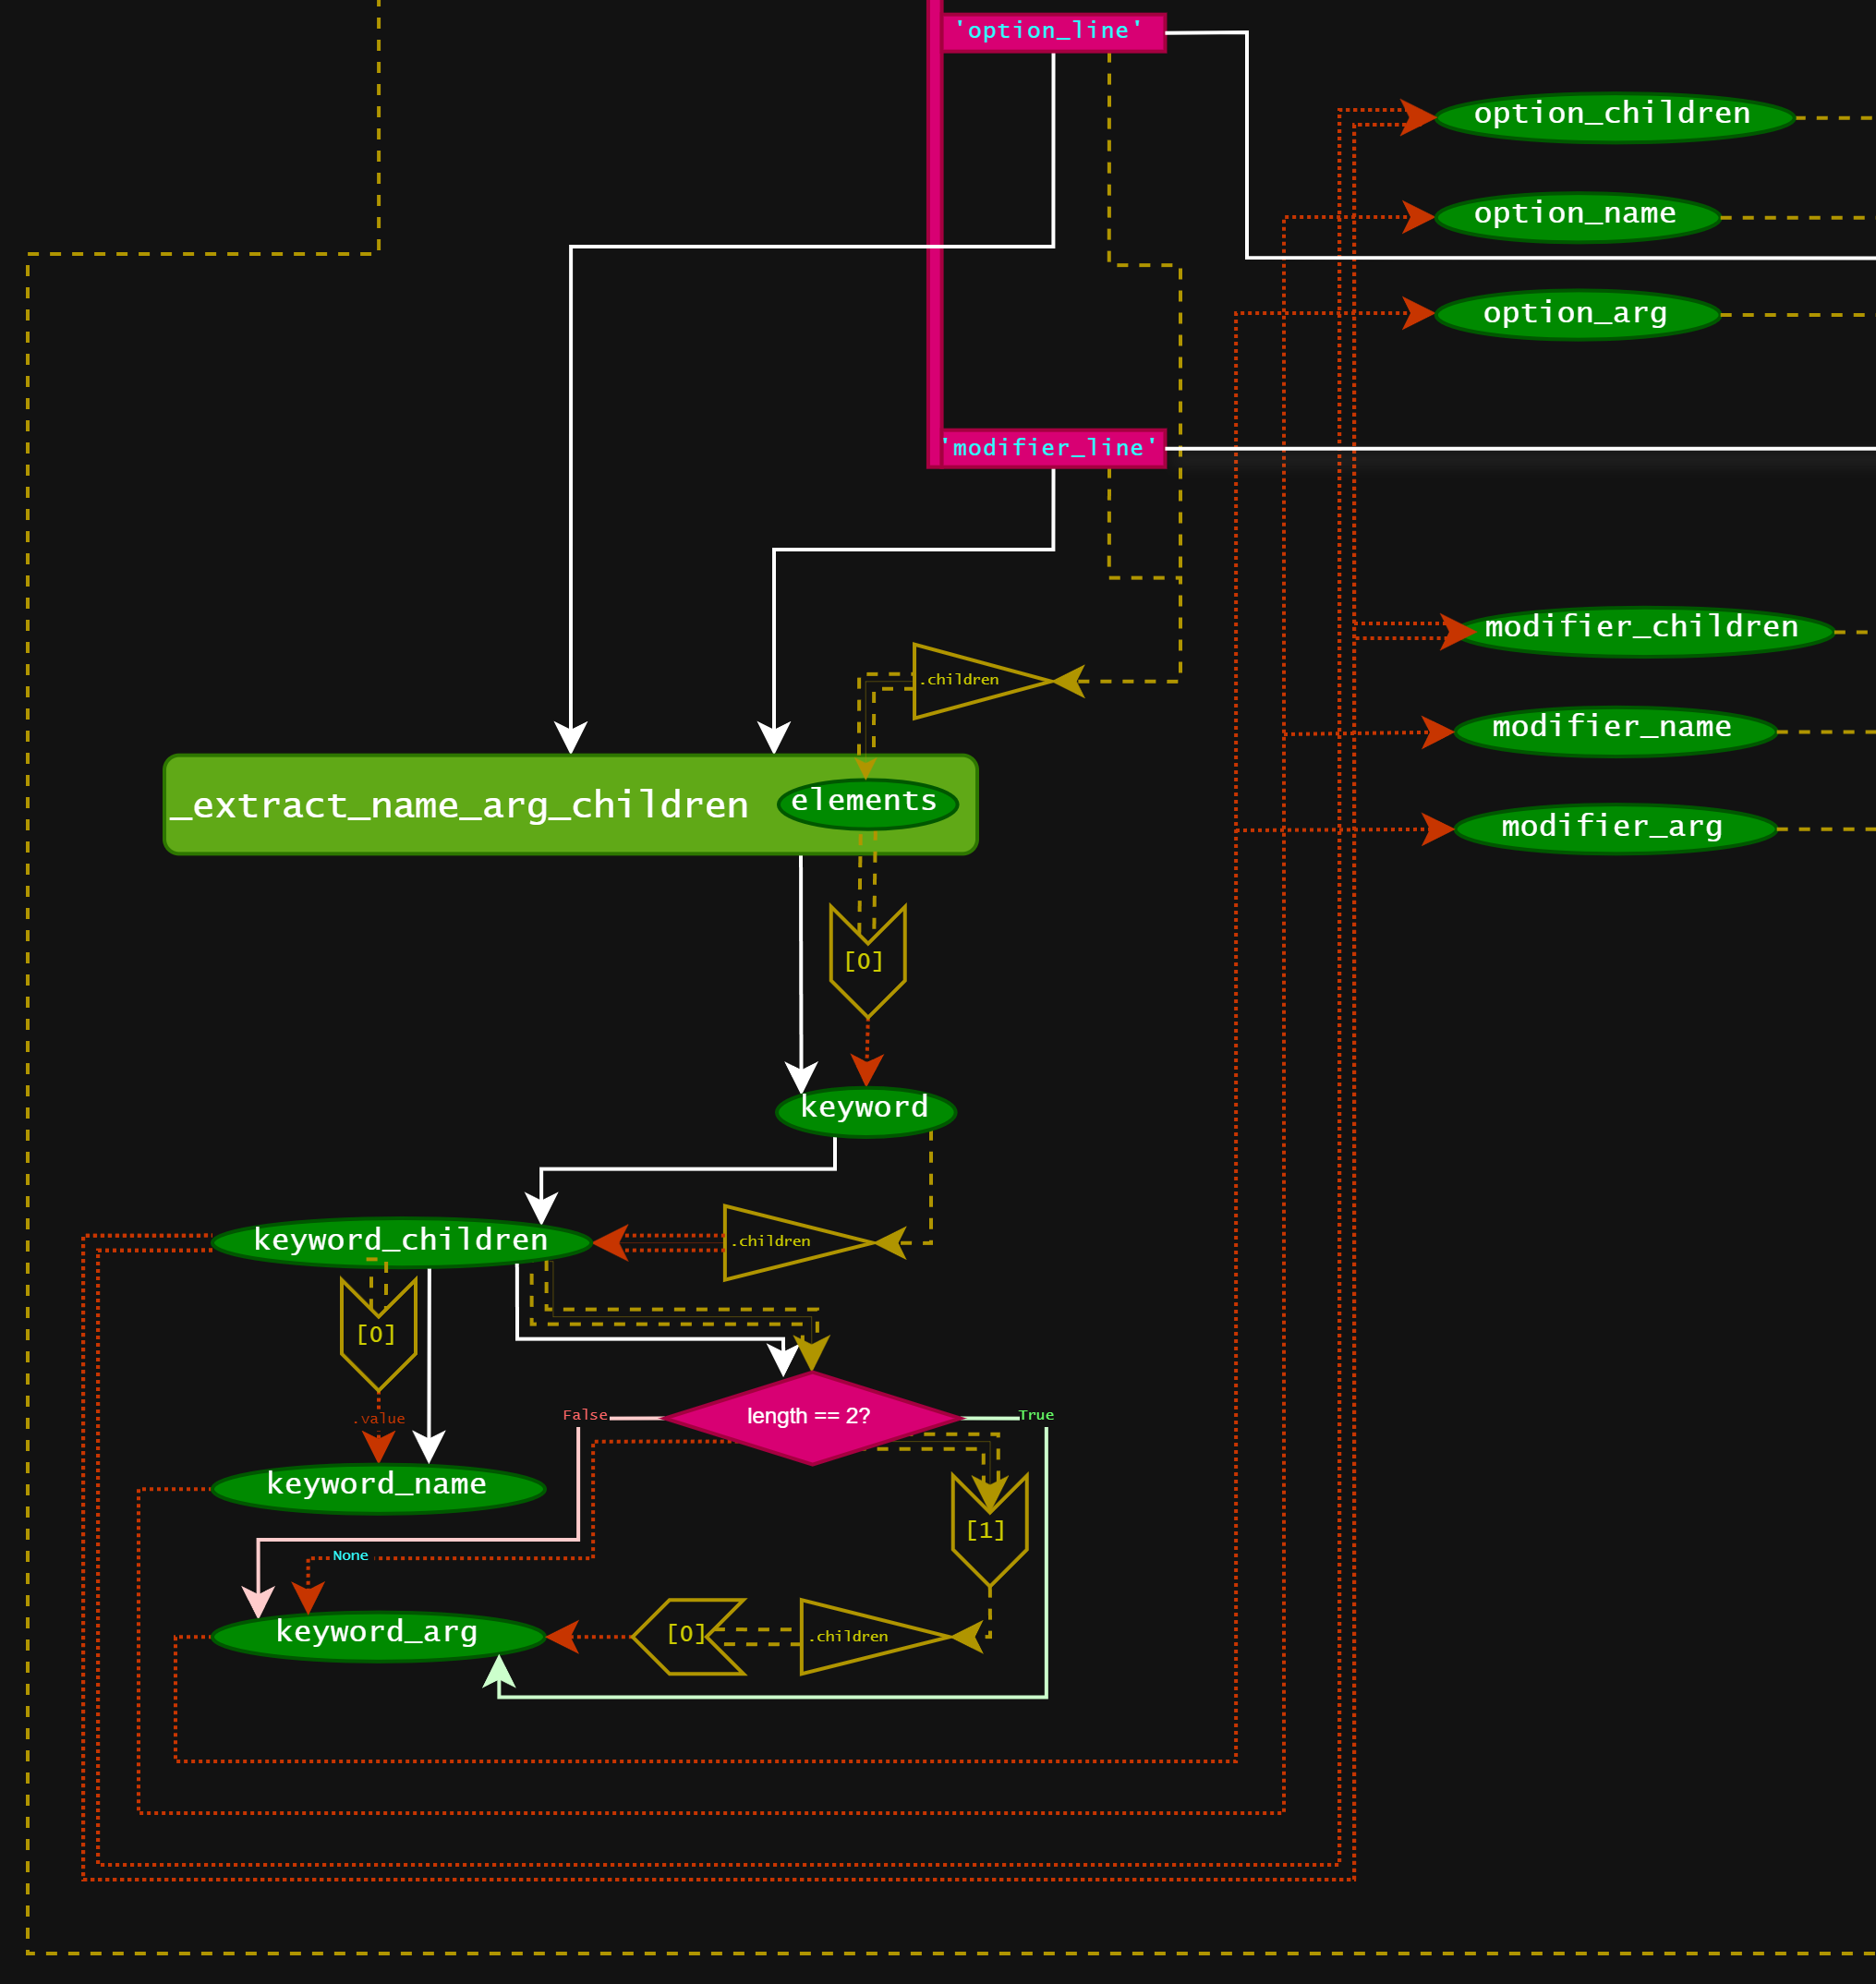
\includegraphics[width=0.8\linewidth]{pics/parser-flowchart/extract-name-arg-children.png}
        \caption{The detailed part of the parser's flowchart diagram which illustrates the extract-name-arg-children procedure.}
        \label{fig:parser-flowchart_extract-name-arg-children}
    \end{subfigure}

    \vspace{6pt}

    \begin{subfigure}[b]{\linewidth}
        \centering
        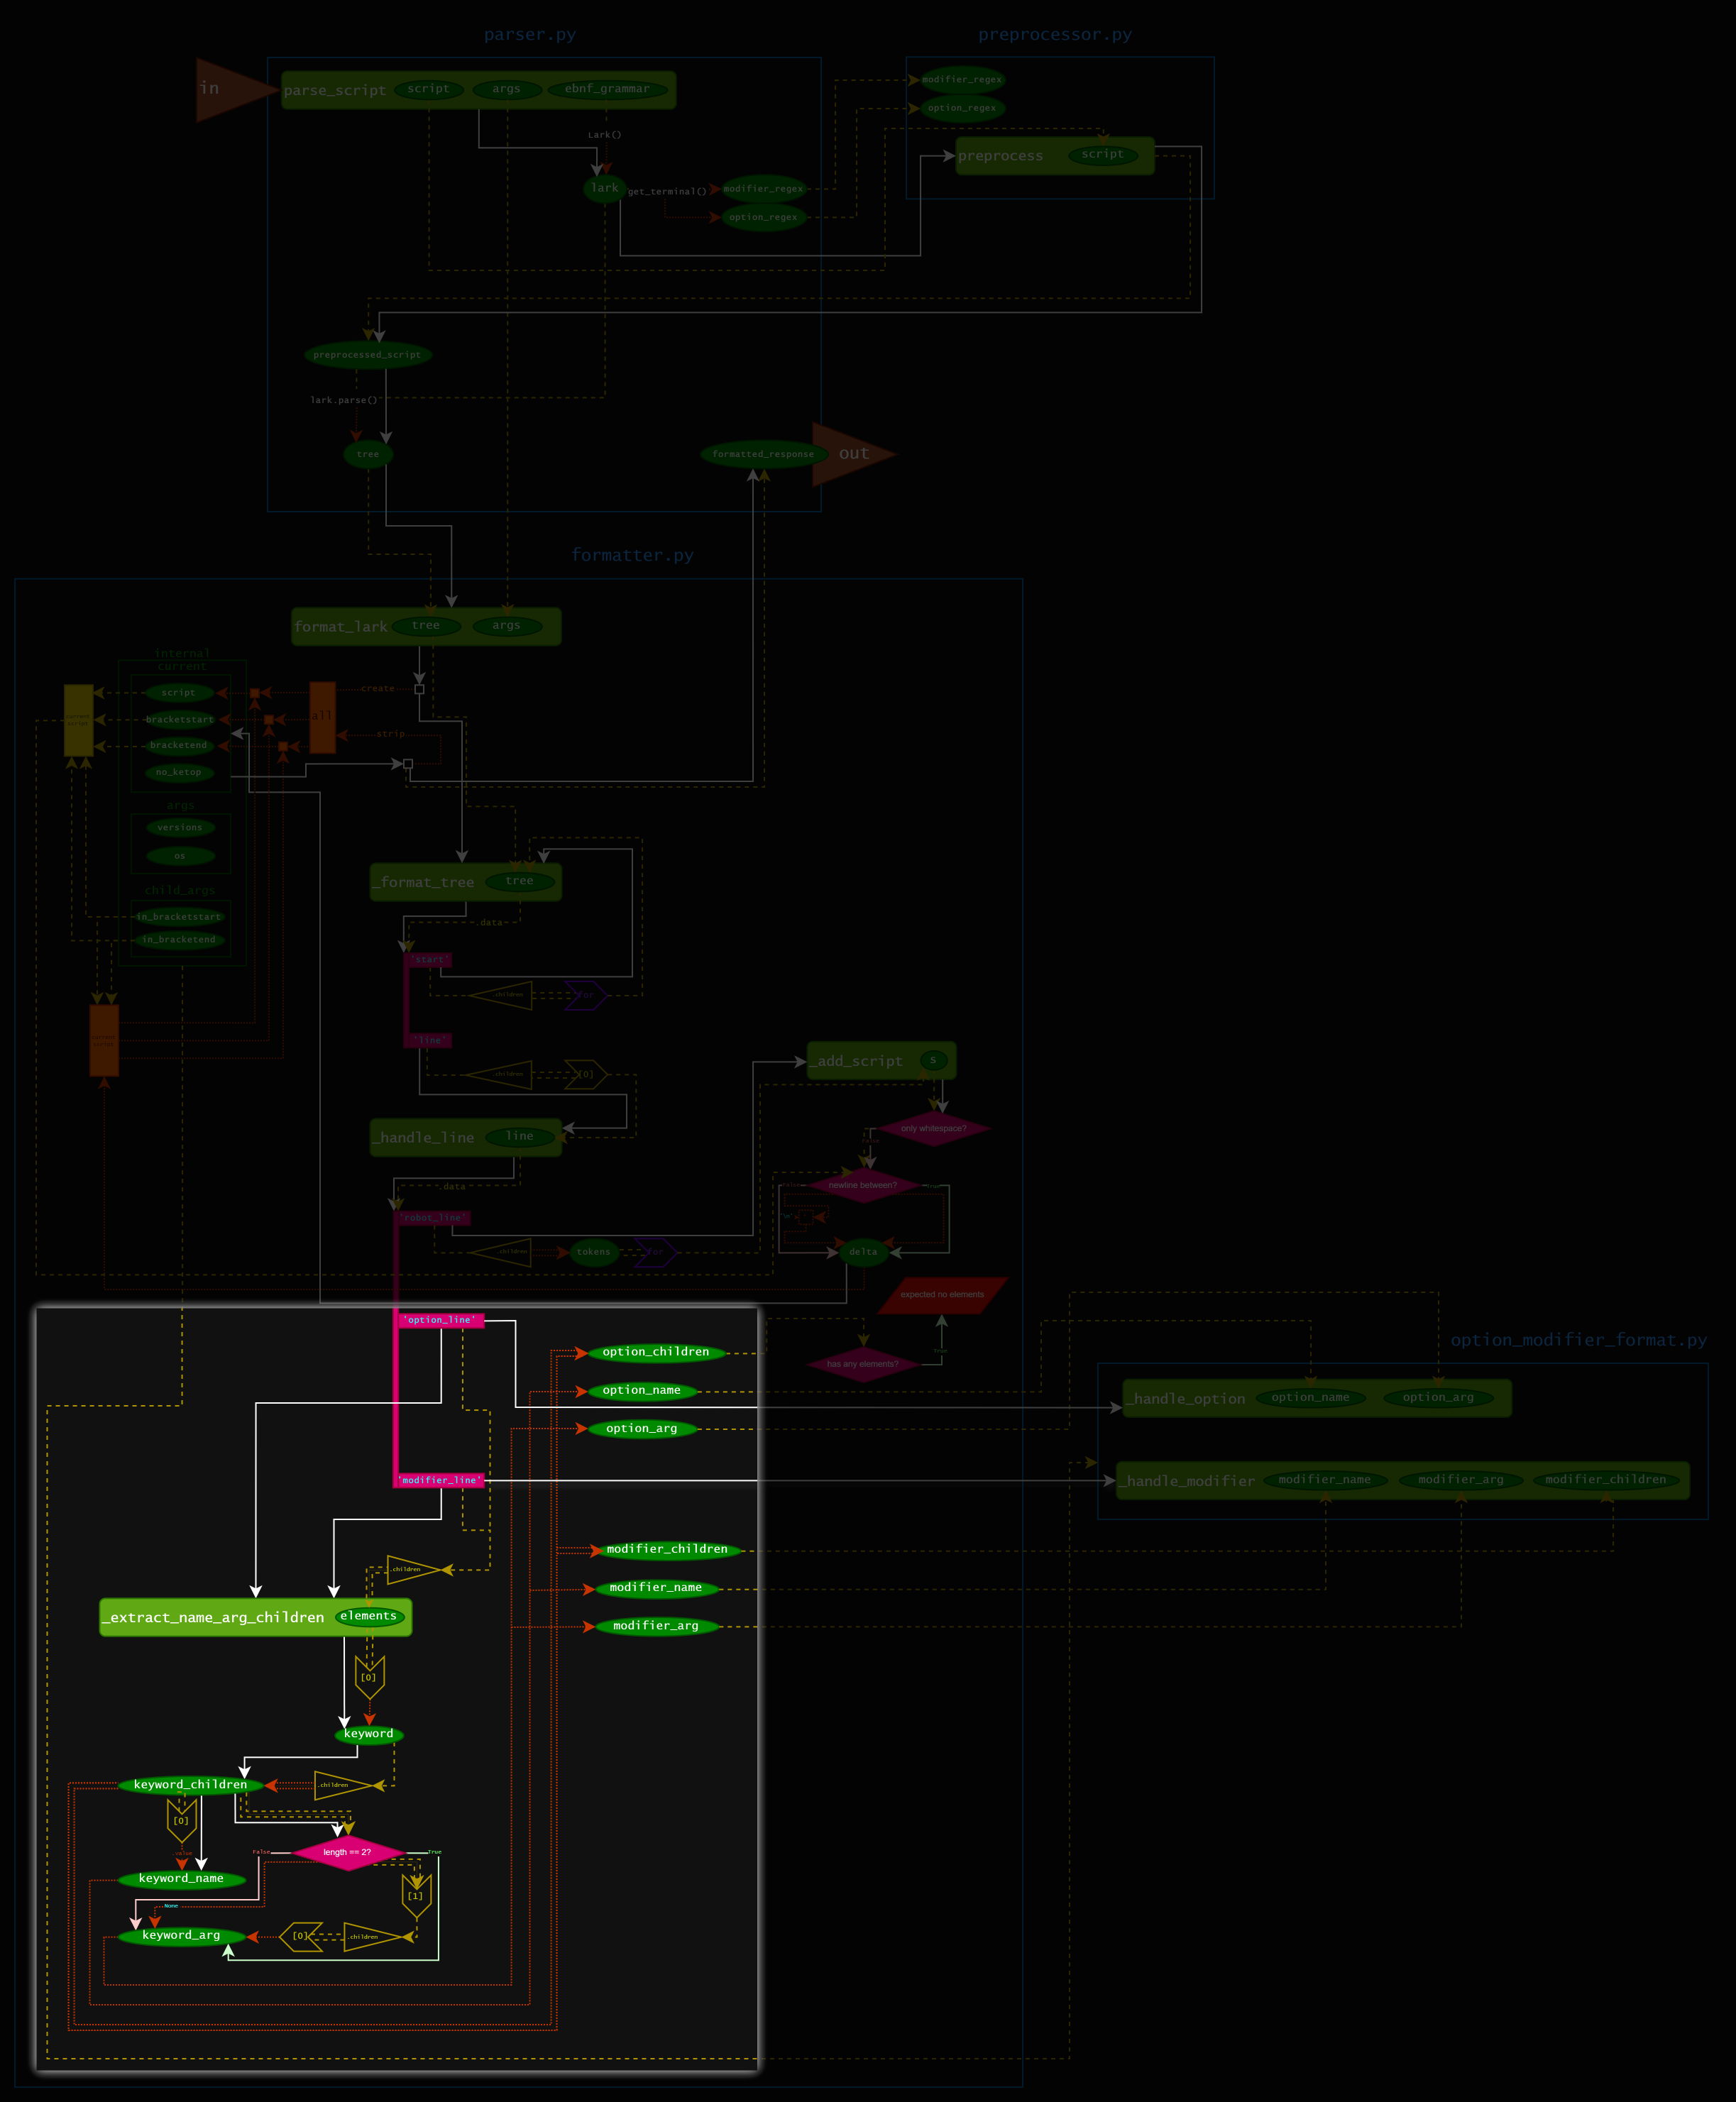
\includegraphics[width=0.35\linewidth]{pics/parser-flowchart/extract-name-arg-children_location.png}
        \caption{The location of the detailed inset within the full flowchart as seen in Figure~\ref{fig:parser-flowchart_full}.}
        \label{fig:parser-flowchart_extract-name-arg-children_location}
    \end{subfigure}

    \caption{The part of the flowchart diagram from Figure~\ref{fig:parser-flowchart_full_combined} that details the extract-name-arg-children procedure of the parser.}
    \label{fig:parser-flowchart_extract-name-arg-children_combined}
\end{figure}



\chapter{Option/Modifier Format [F]}\label{chap:option-modifier-format}
\setauthor{Filip Schauer}
This chapter highlights the implementiation of how options and modifiers are handled by the parser. 

The \verb|OptionModifierFormat| class is used to handle specific keywords. It includes two main functions, which are \verb|handle_option| and \verb|handle_modifier|. Each of these functions matches for its respective name. 

\section{Option @NO\_KETOP}

When encountered, the \verb|no_ketop| variable gets enabled in the \verb|current| \\(\verb|FormattedResponse|).

If that variable has already been set to true (i.e.\ if \verb|@NO_KETOP| was used twice in the file) a warning will be logged.

The \verb|@NO_KETOP| option expects no argument. 

\section{Modifier @VERSION}

TODO

\section{Modifier @OS [F]}

The \verb|@OS| modifier represents a conditional statement and requires an argument. 

The argument represents the operating system to check; it is compared against the \verb|os| variable provided in \verb|FormatterArgs|. This comparison is case-insensitive ignores any leading whitespace. 

If the provided \verb|os| variable is \verb|None|, a warning will be logged and the body gets discarded. 

If the comparison is satisfied, the body will be further recursively parsed; otherwise, the body will be discarded.

\section{Modifier @PREAMBLE [F]} 

The \verb|@PREAMBLE| modifier continues to recursively parse the body text, however the parsed text will be appended to the respective index of \verb|preamble_dict|, as opposed to \verb|script|. This index is given by the required argument.

This is done by returning a \verb|ChildArgs| instance with the \verb|preamble_index| variable set to that given by the argument. 

A syntax exception will be thrown if it is defined inside \verb|@BRACKETSTART|, \verb|@BRACKETEND| or another instance of \verb|PREAMBLE|.

\section{Modifiers @BRACKETSTART and @BRACKETEND [F]}

The \verb|@BRACKETSTART| or \verb|@BRACKETEND| modifier continue to recursively parse the body text, however the parsed text will be appended to \verb|bracketstart| or \verb|bracketend| respectively, as opposed to \verb|script|. 


This is done by returning a \verb|ChildArgs| instance with \verb|in_bracketstart| or \\\verb|in_bracketend| respectively set to \verb|True|.

A syntax exception will be thrown if it is defined inside \verb|@BRACKETSTART|, \verb|@BRACKETEND| or \verb|@PREAMBLE|.

The \verb|@BRACKETSTART| and \verb|@BRACKETEND| modifiers expect no argument.


\chapter{Exceptions and Logging [F]}\label{chap:exceptions-and-warnigs}
\setauthor{Filip Schauer}
% !TEX root = ../../thesis.tex

This chapter will explain how the preprocessor and parser handle exceptions and logging. 

\section{Logging}

In programming, logging is the process of recording information during the execution of a program. It is commonly considered to be an important part of an application, because it allows for issues to be diagnosed and debugged, monitoring performance and application health, analyzing usage patterns and more~\cite{logging}.

In Script Assembler, most things are logged using Python's \verb|logging| module, which had already been set up to work in the \gls{trp} project before the Script Assembler project was started on. 

This module allows for logging on multiple \textit{levels}~\cite{py-logging}. The levels that we utilized in Script Assembler are as follows:

\begin{itemize}
    \item \verb|debug|: We use this level to log nearly every step that the parser takes. As the name suggests, it is useful for debugging purposes, when it might be crucial to consider the exact steps that were taken.
    \item \verb|info|: We use this level for anything that might be \textit{useful to know} regarding the overall flow of the program, that is not critical or necessarily important to consider. It is used, for instance, when the body from a conditional modifier, such as \verb|@VERSION|, is discarded.
    \item \verb|warning|: We use this level to notify the user about situations that, despite not being exceptions, might not be intentional or entirely logical, and could therefore have unforeseen consequences. It is used, for instance, when an option that merely sets a single flag to a value, like \verb|@NO_KETOP|, is used multiple times in the same script. 
\end{itemize}

In this section, the only log level we will be taking an in-depth look at in this thesis is \verb|warning|, as it may provide insight into certain edge cases. 

\subsection{Warnings}

The following is a list of all warnings of \verb|OptionModifierFormat| a user may run into when using the parser:

\begin{itemize}
    \item \textit{NO\_KETOP flag has already been set for this file}: This warning is raised when the \verb|@NO_KETOP| option is used and the \verb|no_ketop| variable is already set to true from a previous use of the option in the same file. In this case, the flag remains enabled. 
    \item \textit{Version for \{\ldots\} is not provided. Discarding block}: This warning is raised when the \verb|@VERSION| modifier is called and the module given in the argument has not been provided in the \verb|versions| dictionary of \verb|FormatterArgs|. That modifier's body gets discarded.
    \item \textit{Provided OS is None. Discarding block}: This warning is raised when the \verb|@OS| modifier is used and the \verb|os| variable of \verb|FormatterArgs| is \verb|None|. That modifier's block gets discarded.
    \item \textit{Provided OS is None. Discarding block}: This warning is raised when the \verb|@OS| modifier is used and the \verb|os| variable of \verb|FormatterArgs| is \verb|None|. That modifier's block gets discarded.
    \item \textit{Provided actual version (\{\ldots\}) is not in a valid semantic version format (https://semver.org/); trying to force parse\ldots}: This warning is raised when the \verb|@VERSION| modifier is called with an argument with a version that is not a valid semantic version format. When this happens, \verb|semantic_version|'s \verb|Version.coerce| function is used, which attempts to correct the version string. If this fails, a \verb|ParserSyntaxError| is raised.
\end{itemize}

Many of the warnings above were requirements given by our project partner.

\section{Exceptions}

In programming, when the normal flow of a program is disrupted, an exception often gets thrown. Aside from built-in exceptions like when attempting to divide a number by zero, Python also allows for defining custom exceptions. This can be useful to, for instance, improve the clarity of error messages, make it easier to diagnose issues, and to avoid code duplication~\cite{py-exceptions}. 

In this chapter, the terms \textit{exception} and \textit{error} are used interchangeably. 

The exceptions \verb|ParserSyntaxError| and \verb|ParserInternalError| have been created for use in the parser and the preprocessor, and they are defined as the following:

\begin{lstlisting}[language=Python, caption={Class definitions of \texttt{ParserSyntaxError} and \texttt{ParserInternalError}.}, label={lst:class_definition_parser_syntax_internal_error}]
class ParserSyntaxError(Exception):
    message:str
    def __init__(self, message)->None:
        super().__init__(message)
        self.message = message

class ParserInternalError(Exception):
    message:str
    def __init__(self, message)->None:
        super().__init__(message)
        self.message = message
\end{lstlisting}

These exceptions are specified to be used for the following purposes:

\begin{itemize}
    \item When the use of a keyword or its related option/modifier syntax does not match specification, or when there is an attempt to use a keyword that is not recognized by the parser, a \verb|ParserSyntaxError| should be thrown. 
    \item When an internal problem prevents the parser or preprocessor from being able to continue in an intended way, a \verb|ParserInternalError| should be thrown. However, it is important to note that, ideally, the code should instead be written in a way that makes getting such exception impossible, as any unusual part of the input text should be handled by specified \verb|ParserSyntaxError|s. 
\end{itemize}

While neither of these exceptions have been used rigorously, many different scenarios have been considered and tested to prevent falsified or otherwise unhelpful results from the Script Assembler. 

For a user of our project, it might be important to be aware of the possible exceptions that are intended for them to run into if something is found to be syntactically incorrect. For this reason, what follows is a list of occasions that would raise a \verb|ParserSyntaxError|:

\begin{itemize}
    \item Usage of the \verb|@END| keyword which is reserved for internal purposes.
    \item Defining a modifier with no body.
    \item Usage of a keyword that the parser does not recognize. 
    \item Omitting the argument for a keyword that requires one. This includes \verb|@VERSION|, \verb|@OS|, and \verb|@PREAMBLE|.
    \item Including an argument for a keyword that does not allow for one. This includes \verb|@NO_KETOP|, \verb|@BRACKETSTART|, and \verb|@BRACKETEND|.
    \item Defining a \verb|@PREAMBLE|, \verb|@BRACKETSTART|, or \verb|@BRACKETEND| inside of the body of a \verb|@PREAMBLE|, \verb|@BRACKETSTART|, or \verb|@BRACKETEND|.
    \item The argument of the \verb|@VERSION| modifier not being made up of three parts each seperated by a space.
    \item The comparator given in the \verb|@VERSION| modifier is not valid.
    \item If \verb|semantic_versioning| fails to parse a version number to semantic version format after trying to force parse with \verb|Version.coerce|.
    \item When Lark runs into \textit{unexpected characters} and is therefore not able to match the remaining characters to a terminal~\cite{py-module-lark-api}.
    \item When Lark runs into an \textit{unexpected end of file} when it would still expect a token~\cite{py-module-lark-api}.
\end{itemize}


\chapter{TRP-Integration [X]}\label{chap:trp-integration}
\setauthor{Axel Csomány}
% !TEX root = ../../thesis.tex

The following section will focus on two aspects, namely the usage of the testing environment and the assembling of the final script, which occurs in the background.

\section{Using The Testing Environment}

The user interface of the testing environment has initially been designed to give the user the ability to easily monitor which test cases are present in the system and to quickly run a custom selection of these test cases. 

The test cases are displayed in a makeshift file explorer, which organizes the test cases in a hierarchical structure based on their respective test suites and sections. Checkboxes are provided next to each test case, as well as next to each test suite and section, allowing the user to easily select or deselect entire groups of test cases. Once the user selected a batch of test cases, they can give the test run a name and click to start the test run. 

Once the test run is started, the Script Assembler is responsible for which test cases should actually be included in the final script and in which order they should be placed. These decisions are based on the presence of the keywords in the test cases, as well as the order in which they are selected by the user. Once the final script is assembled, it is ready to be executed in the testing environment, and the results can be analyzed by the user upon completion. 

\section{Assembling The Script}

The \textit{casemanager.py} module is responsible for the handling and management of test cases within the system. Considering the new features and improvements that have been implemented, this module has undergone significant changes. The following subsections will provide a detailed overview of the modifications made to the \textit{casemanager.py} module, in form of code snippets and explanations.

The function that is responsible for assembling the final script has undergone the most significant changes, considering that it is not only one of the most important functions in the module, but also because our work targets the functionality of this function directly. This is because the new features include keywords such as PREAMBLE, BRACKETSTART and BRACKETEND, which explicitly alter the way the script is assembled. Furthermore, other functionalities have been modified to fit the new features.

\subsection{Detecting Keywords}

\begin{lstlisting}[language=Python, caption={Old: Checking for NO\_KETOP keyword in script}, label={lst:old_no_ketop}]
    if "@NO_KETOP" in script:
        log.warning("found NO_KETOP in test case.")
        script = script.replace("@NO_KETOP", "")
        variables["NO_KETOP"] = True

\end{lstlisting}

In listing~\ref{lst:old_no_ketop}, the old code checks for the presence of the NO\_KETOP keyword in the script directly, and if it is foung, it is removed from the script and a corresponding variable is set to True. This approach is straightforward and works well enough for the old functionality, but it does not take into account any new features that may be added in the future. Since the expandability of the system is a key aspect of our work, this approach has been modified.

\begin{lstlisting}[language=Python, caption={New: Checking for NO\_KETOP keyword in script}, label={lst:new_no_ketop}]
    if formatted.no_ketop:
        if variables['NO_KETOP']:
            log.warning('NO_KETOP flag has already been set for this test case')
        variables['NO_KETOP'] = True
\end{lstlisting}

In listing~\ref{lst:new_no_ketop}, the new code checks for the presence of the NO\_KETOP keyword in a more structured way, by using a formatted object that contains all the relevant information about the given script. This includes the presence of a BRACKETSTART or BRACKETEND keyword. This approach allows the functionality of the test script format to be more extendable, as data pertaining to a new keyword can easily be added to the formatted object without having to modify the core logic of the script assembly process.

Additionally, the new code also includes a check to ensure that the NO\_KETOP flag has not already been set for the given test case, since that unintended behavior would indicate a potential issue in the system.

\begin{lstlisting}[language=Python, caption={Old: Checking for BRACKETSTART and BRACKETEND keyword in script}, label={lst:old_bracket_keywords}]
    script_lines = script.splitlines()          
        if script and "@BRACKETSTART" in script_lines[0]:

            brackets = script.replace("@BRACKETSTART", "").split("@BRACKETEND")

            start += f"\nT{tc.tr_test_id} - {tc.tr_case.title} [BRACKET START]\n"
            start += brackets[0]

            end += f"\nT{tc.tr_test_id} - {tc.tr_case.title} [BRACKET END]\n"
            end += brackets[1]
\end{lstlisting}

The check for the BRACKETSTART and BRACKETEND keywords worked similarly to the NO\_KETOP keyword, as shown in listing~\ref{lst:old_bracket_keywords}. The script was split into lines. If the first line contained the BRACKETSTART keyword, the script was split into two parts using the BRACKETEND keyword as a delimiter. The first part was added to the start variable, while the second part was added to the end variable. The identical problems that were present in the NO\_KETOP keyword check arise here as well.

\begin{lstlisting}[language=Python, caption={New: Checking for BRACKETSTART and BRACKETEND keyword in script}, label={lst:new_bracket_keywords}]
    if formatted.bracketstart != '':
        start += f"\nT{tc.tr_test_id} - {tc.tr_case.title} [BRACKET START]\n"
        start += self._add_tab(formatted.bracketstart) + '\n'
    if formatted.bracketend != '':
        end += f"\nT{tc.tr_test_id} - {tc.tr_case.title} [BRACKET END]\n"
        end += self._add_tab(formatted.bracketend) + '\n'
\end{lstlisting}

As shown in listing~\ref{lst:new_bracket_keywords}, the bodies of the BRACKETSTART and BRACKETEND keywords are now stored in the formatted object as separate variables after the script has been parsed. The contents of these variables are then added to the start or end variable respectively, if they are not empty.

\subsection{Ordering of Scripts}

The initial implementation of the script assembly consisted of three variables that were used to store the different parts of the script, namely:

\begin{itemize}
    \item \textit{start}: \\
    This variable was used to store the scripts that contained the BRACKETSTART keyword.

    \item \textit{regular}: \\
    This variable was used to store the scripts that did not contain any of the special ordering keywords.

    \item \textit{end}: \\
    This variable was used to store the scripts that contained the BRACKETEND keyword.
\end{itemize}

This approach worked well enough and has been extended in the new implementation, now featuring an additional variable called \textit{preamble}, which contains all scripts that contain the PREAMBLE keyword in the correct order. This variable is placed first in the final assembly of the script. 

\begin{lstlisting}[language=Python, caption={Old: Finding and inserting regular scripts}, label={lst:old_regular_script}]
    elif script != "":
        regular += f"\nT{tc.tr_test_id} - {tc.tr_case.title}\n"
        regular += script
\end{lstlisting}

If the script did not contain any of the special ordering keywords, it arrives at the code shown in listing~\ref{lst:old_regular_script} and is added to the regular variable. 

\begin{lstlisting}[language=Python, caption={New: Finding and inserting regular scripts}, label={lst:new_regular_script}]
    if formatted.script != '':
                regular += f"\nT{tc.tr_test_id} - {tc.tr_case.title}\n"
                regular += self._add_tab(formatted.script) + '\n'
\end{lstlisting}

In the new implementation, the code simply checks if the script variable in the formatted object is not empty. Scripts that do not contain any of the special ordering keywords are stored in this variable, and if it exists, it is added to the regular variable. 

\begin{lstlisting}[language=Python, caption={New preamble variable and final assembly of the script}, label={lst:final_assembly}]
    preamble: str = ""
    for preamble_key in sorted(robot_preamble_dict.keys()):
        preamble += f"\nT{preamble_test_metadata[preamble_key][0]} - {preamble_test_metadata[preamble_key][1]} [PREAMBLE]\n"
        preamble += self._add_tab(robot_preamble_dict[preamble_key]) + '\n'

    combined_script = preamble + start + regular + end
\end{lstlisting}

In listing~\ref{lst:final_assembly}, the new preamble variable is created by iterating through the \textit{robot\_preamble\_dict}, which is a dictionary containing the bodies of all the PREAMBLE keywords, and adding the contents of these keywords to the preamble variable. This dictionary is already ordered by the index of each PREAMBLE keyword, making sure that the preamble variable is assembled correctly. This step happens after the start, regular and end variables have been completely assembled, leading into the final assembly of the script, which is a combination of all four variables.



\chapter{Syntax Highlighting [A]}\label{chap:syntax-highlighting}
\setauthor{Adam Höllerl}
\section{Introduction}

One part of this project presented in this theis, was the development of Syntax Highlighting. As already described in previous chapters, the Script Assembler works by overlaying a custom syntax on top of the standard Robot Framework language using an EBNF grammar, thus allowing annotations like \texttt{@VERSION} or \texttt{@BRACKETSTART}.

There is a fundamental problem though. Because standard text-editors and native Robot Framework syntax highlighters do not recognize this new grammar, custom annotations would be displayed as plain text, or worse, marked as syntax errors.

For KEBA, the frontend editor needs a way to visually mark these custom elements, because if they are not able to do so, it can lead to worse developer experience and more errors that go unnoticed until execution. Without visual validation, developers make more syntax mistakes. 
eFor example, writing \texttt{@VERISON} instead of \texttt{@VERSION} or using an invalid argument type, like passing a plain string where a semantic version number is expected, would not be recognized while typing. These mistakes remain unnoticed. The errors are only found during the backend transpilation phase much later, when an error log is generated. This breaks the entire programming workflow and wastes precious time.

To fix this, custom syntax highlighting should be integrated into the web-based pre-existing code editor. The main objective simply was to get immediate visual feedback and validation. Correct keywords, different types of arguments and errors should all be highlighted in unique colors. This should reduce the time needed for test development, with our Script Assembler annotations/modifiers in use, by a lot. Figure \ref{fig:syntax_highlighting} shows how the editor is supposed to handle valid and invalid inputs.

\begin{figure}
    \centering
    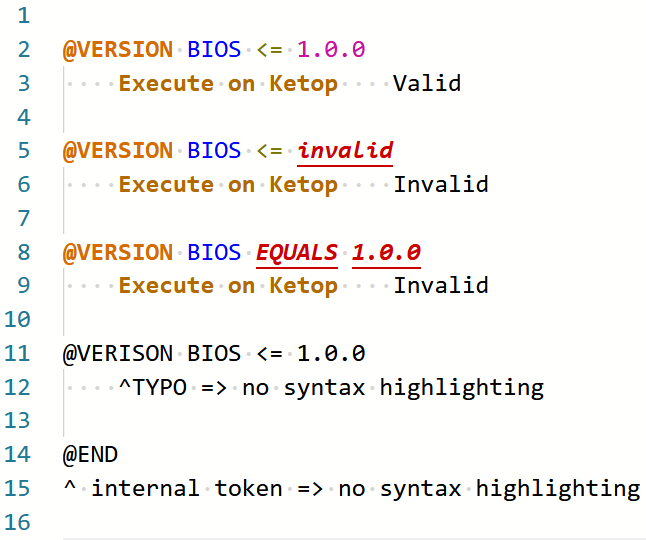
\includegraphics[width=0.75\linewidth]{pics/SyntaxHighlighting/SyntaxWHITE.png}
    \captionsetup{justification=centering,singlelinecheck=false}
    \caption{
      Syntax Highlighting in Action\\
{\small\itshape (color scheme was modified for better visibility in print)}}    
    \label{fig:syntax_highlighting}
\end{figure}

\section{Monaco Editor Setup}

The frontend application already used the Monaco Editor to provide basic syntax highlighting for standard Robot Framework scripts with the Monarch library \cite{MonacoGithub, MonacoMonarchDocs}.
Monaco is the underlying technology of Visual Studio Code and can be used in frontends through packages. The package that was used was outdated and a few other architectural issues had to be fixed, before the syntax highlighting could be implemented.

\subsection{Legacy Version Conflicts}

Over time the frontend ecosystem of the project has been updated to Angular 15, but the existing editor integration was still based on the widely used wrapper library \texttt{ngx-monaco-editor}. Unfortunately, this specific package was no longer being updated.  It officially only supported Angular up to version 12 \cite{DeprecatedNgxMonaco}. Previously developers used the npm force flag during installation to make the project compile using this already deprecated package, bypassing the dependency conflicts.

This workaround made it possible for the legacy code to somehow continue working, but it also created major risks for maintainability and the build process. Forcing npm installation is a bad practice since it only covers up package mismatches and other errors. Because of this, there is a major risk that one might get unpredictable runtime behaviors \cite{npmForceDocs}. Since we do not want that, especially later on in production, the package needed to be replaced.

After some research, the best and most widely used package, fitting exactly our requirements, seemed to be \texttt{ngx-monaco-editor-v2}. This version is an actively maintained community fork that is compatible with mordern Angular versions \cite{NgxMonacoEditorV2}.

The migration was handled in several steps to ensure a stable base. The \texttt{package.json} had to be updated, then the \texttt{app.module.ts} was refactored to match the new library and finally the asset paths in \texttt{angular.json} had to be updated.

\subsection{Custom Theme}

A custom Monaco theme was required to map the custom syntax to the correct colors. The requirement for that theme, was for the colors to stand out compared to the standard Robot Framework syntax.

The editor worked fine with its predefined default designs, but as soon as a newly created custom design was applied, a runtime error occurred: \texttt{Uncaught TypeError: this.themeData.colors is undefined}. This error completely stopped the editor from rendering any custom syntax highlighting.

Looking in the documentation gave me a hint in the right direction. The engine of Monaco is rather strict, so a \texttt{colors} object has to be provided for a theme, even if it is empty and never used \cite{MonacoThemeColorsAPI}. 

The solution was to add an empty \texttt{colors} object to the theme definition. Listing \ref{lst:theme_definition} shows the working theme configuration, which includes the required \texttt{colors} property alongside the specific token rules.

\begin{lstlisting}[caption={Custom monaco theme including the required color object}, label={lst:theme_definition}, float=htbp]
// Definition of the custom language theme
(<any>window).monaco.editor.defineTheme('robot-theme', {
  base: 'vs-dark',
  inherit: true,
  rules: [
    { token: 'variables', foreground: '#9CDCFE' },
    { token: 'keywords', foreground: '#ffe18f', fontStyle: 'bold' },
    { token: 'modifier', foreground: '#f09c00', fontStyle: 'bold' },
    { token: 'invalid', foreground: '#ff0000', fontStyle: 'underline italic' },
    // [...]
  ],
  colors: {} // Required to prevent 'this.themeData.colors is undefined'
});
\end{lstlisting}

\section{Monarch Lexer for Custom Annotations}

After the editor and theme were successfully configured, the core task was to define the syntax rules for the custom grammar of the Script Assembler. The already in use Monaco Editor uses Monarch for syntax highlighting, which works declaratively. Developers define lexers using JSON configuration objects instead of writing complex parser code \cite{MonacoMonarchDocs}.

\subsection{Tokenization and State Machine}

Monarch basically just uses Regex to handle the tokenization. The step-by-step-process starts with the lexer, that reads the document text in order and tries  to match the defined regular expression patterns. When it finds a match, the matched text is assigned a specific token class. This can be a specific keyword or a comment or it could also just be a newly defined custom modifier. The editor then maps these token classes to the specific color values defined in the active theme.

A global list of Regex rules is sufficient for simple languages. But for the custom annotations there is a need for context-aware parsing. For example, the arguments that follow an \texttt{@VERSION} annotation should be highlighted, but if the same argument is written in a comment it should not.

Monarch's state machine solved this problem. The lexer starts in a default \texttt{@root} state, when a specific pattern is matched, the lexer jumps into a different, explicitly defined state, and different Regex rules apply in this new state.

\subsection{Handling Modifiers and Arguments}

The annotations can be roughly divided into two categories. Those without any arguments and those with specific argument structures.

Modifiers without arguments, such as \texttt{@BRACKETSTART}, are simple to implement. As shown in Listing \ref{lst:root_tokenizer}, when the lexer encounters this keyword, it transitions to an \texttt{@endOfLine} state. This state  makes sure that no more text is accepted on this line. 

\begin{lstlisting}[caption={Monarch tokenizers root state}, label={lst:root_tokenizer}, float=htbp]
tokenizer: {
  root: [
    // Standard Robot Framework variables
    [/[\$@]\{[\w_/]+\}/, 'variables'],

    //#region MODIFIERS
    [/@(?:PREAMBLE)\b/, 'modifier', '@preambleArg'],
    // Modifiers without any arguments transition to @endOfLine
    [/@(?:BRACKETSTART|BRACKETEND)\b/, 'modifier', '@endOfLine'], 
    // Modifiers with complex arguments transition to their specific states
    [/@(?:VERSION)\b/, 'modifier', '@versionArgsIdentifier'],
    [/@(?:OS)\b/, 'modifier', '@osArg'],
    //#endregion
    
    // [...]
  ],
// ...
\end{lstlisting}

Modifiers with arguments are more difficult, because hey require a more complex sequence of state transitions. The modifier \texttt{@VERSION} is a good example of this as the version check needs three different components. Also important is,  they have to be in an exact order, starting with an identifier (the BIOS or software name), than a comparison operator (e.g., <, >=), and at last a valid semantic version string.

A chain of states was implemented, Root to identifier, Identifier to operator, Operator to version. That means that when \texttt{@VERSION} is found in the \texttt{@root} state, the lexer transitions to \texttt{versionArgsIdentifier}. Once a valid word is found there, it transitions to \texttt{versionArgsOperator} and finally to \texttt{versionArgsSemver}.

This ``state machine'' approach guarantees that the syntax highlighting exactly fits to the strict sequence that the parser needs. Listing \ref{lst:version_states} shows this state chain in detail. 

\begin{lstlisting}[caption={State transitions for the \texttt{@VERSION} modifier}, label={lst:version_states}, 
  breaklines=true, breakatwhitespace=false, float=htbp ]
versionArgsIdentifier: [ 
  // Entry point: match a word, then proceed to operator state
  [/[\w_]+/, 'arg.word', '@versionArgsOperator'],
  [/\n/, 'invalid', '@root'],
  [/./, 'invalid']
],
versionArgsOperator: [
  // Match comparison operators, then proceed to semantic version state
  [/(?:[<>]=?)|(?:[!=]=)/, 'arg.operator', '@versionArgsSemver'],
  [/\n/, 'invalid', '@root'],
  [/./, 'invalid']
],
versionArgsSemver: [
  // Match standard semantic versioning format
  // https://semver.org/#is-there-a-suggested-regular-expression-regex-to-check-a-semver-string
  [/(0|[1-9]\d*)\.(0|[1-9]\d*)\.(0|[1-9]\d*)(?:-((?:0|[1-9]\d*|\d*[a-zA-Z-][0-9a-zA-Z-]*)(?:\.(?:0|[1-9]\d*|\d*[a-zA-Z-][0-9a-zA-Z-]*))*))?(?:\+([0-9a-zA-Z-]+(?:\.[0-9a-zA-Z-]+)*))?/, 'arg.version'],
  [/\n/, '', '@root'],
  [/./, 'invalid']
],
\end{lstlisting}

The Regex for the semantic version argument might look complicated and hard to maintain, but it is the officially provided Regex by the organization behind semantic versions. 

\section{Troubleshooting and Error Handling}

After solving the correct highlighting of valid syntax, the next tasks were to handle edge cases and wrong inputs. 

During the implementation of the lexer, two main problems appeared, firstly to prevent ``state bleed'' over multiple lines,  secondly to provide visual error feedback without using a dedicated Language Server.

\subsection{Fixing State Bleed}

The custom EBNF grammar for the Script Assembler is strictly line-bound, so an annotation has to be strictly on a singular line. So if a line break occurs the editor should return to the standard context used for the syntax highlighting of the Robot Framework.

In the beginning, this caused a big conflict with Monarch's stateful tokenization. When the lexer goes into a state like \texttt{versionArgsIdentifier}, it just stays inside it until an explicit command such as \texttt{@root} or \texttt{@pop} is triggered. If a developer typed the keyword \texttt{@VERSION} and then pressed the Enter key without any arguments, the lexer got stuck in the \texttt{versionArgsIdentifier} state on the next line. Because of this, normal Robot Framework code on the following lines was wrongly checked against the version argument regular expressions. This completely destroyed the syntax highlighting for the whole rest of the file (see Figure \ref{fig:statebleed} for example).

\begin{figure}[hbtp]
    \centering
    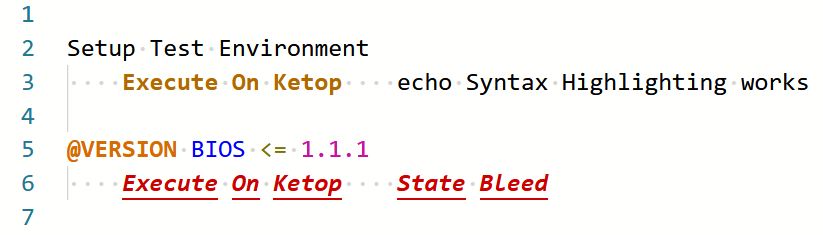
\includegraphics[width=1\linewidth]{pics/SyntaxHighlighting/state-bleed-white.png}
    \caption{State bleed in the editor when line breaks are not included}
    \label{fig:statebleed}
\end{figure}


To fix this ``state bleed'', the lexer had to recognize line breaks as termination triggers. Normally, Monarch works line-by-line and does not pass line break characters to the Regex engine. To change this, the \texttt{includeLF} property was enabled in the language configuration (see Listing \ref{lst:monarch_config_lf}).

\begin{lstlisting}[caption={\texttt{includeLF} in the Monarch config}, label={lst:monarch_config_lf}, float=htbp]
(<any>window).monaco.languages.setMonarchTokensProvider('robot', {
  ignoreCase: true,
  includeLF: true, // Exposes newline to the regex engine
  tokenizer: {
    // tokenizer rules ...
  }
});
\end{lstlisting}

With \texttt{includeLF} set to true, line breaks can be recognized. As can be seen in the state machine definition in Listing \ref{lst:version_states}, each argument state received a new rule for handling the newline character: \texttt{[/\textbackslash n/, 'invalid', '@root']}. Sometimes the lexer just resets to the \texttt{@root} state without marking an error. This is used when a line break is allowed and does not count as a syntax mistake in that specific case. This ensures that a line break always returns the lexer to the \texttt{@root} state and so protects the highlighting of all following code.

\subsection{Visualizing Syntax Errors}

A major goal for the fronted-editor was to show syntax errors to the user right away, but there was a strict rule for this. The error highlighting had to work only through the Monarch configuration, because a complex language server or an extra linter were not an option, as tools like that just use too many resources.

This was quite a problem because Monarch is really just a lexical analyzer, meaning a lexer, and not a semantic parser \cite{MonacoMonarchDocs};~\cite[pp.~5-8]{Aho2006}. It only uses regular expressions to map strings to token classes. It does not know anything about ``errors'' or ``warnings''. It also cannot draw the typical red wavy lines, that are used for code defects in modern \glspl{ide}.

To solve this problem, a visual workaround had to be built with a custom token class called \texttt{invalid}. In the custom Monaco Theme (see Listing \ref{lst:theme_definition}), this category got a unique style with red text-color,  italic style and an underline.

This \texttt{invalid} category then served as a catch-all mechanism in the state machine. Monarch always checks the rules of a state from top to bottom \cite{MonacoMonarchDocs}. By placing the rule \texttt{[/./, 'invalid']} at the very end of a states rule list, any character that does not match the expected valid patterns or the newline reset automatically falls through to this fallback rule.

A good  example for this is the modifier \texttt{@BRACKETSTART}. As it does not allow any arguments, the following happens by running the system. When the lexer sees this exact keyword, it switches to the \texttt{endOfLine} state (see Listing \ref{lst:end_of_line_state}).

\begin{lstlisting}[caption={The \texttt{endOfLine} state}, label={lst:end_of_line_state}, float=htbp]
endOfLine: [
  [/\n/, '', '@root'], // Valid: line ends, return to root
  [/./, 'invalid']     // Error: any other character is invalid
],
\end{lstlisting}

For example for the case, when a developer accidentally types a  \texttt{@BRACKETSTART argument}, the lexer first recognizes the annotation, jumps to the \texttt{endOfLine} state. There, it expects the end of the line. Instead, it encounters a space, and the word ``argument''. Because these characters do not match the \texttt{/\textbackslash n/} Regex, they fall through to the \texttt{/./} rule. As a result, the string ``argument'' turns red, gets underlined and italic, and by doing so, shows the developer a syntax error. The user sees a clear syntax error right away without backend validation. Real-time error feedback is a useful feature, and even better, everything remains strictly within the boundaries of the Monarch lexer architecture.

\section{Limitations}

Being able to catch errors early with the syntax highlighting was definitely worth the addition. But even with all the effort, there is a limitation that could not be fixed, since there is a conflict between the rules of the two used languages, which could only be fixed through a custom Language Server.

The EBNF grammar for the backend is strictly case-sensitive. That means, all annotations and modifiers like \texttt{@VERSION} or \texttt{@OS}, have to be in uppercase, and different spelling leads to  a syntax error during transpilation.

The standard Robot Framework language on the other hand works differently. Here upper and lower case do not matter, the language is case-insensitive \cite{RobotFrameworkCaseInsensitive}. Because of this, the \texttt{ignoreCase} property of the Monarch lexer must be set to true globally, if not, the normal keywords and variables do not get the correct highlighting (see example in Figure \ref{fig:case-sensitivity-issue}). 

\begin{figure}[htb]
    \centering
    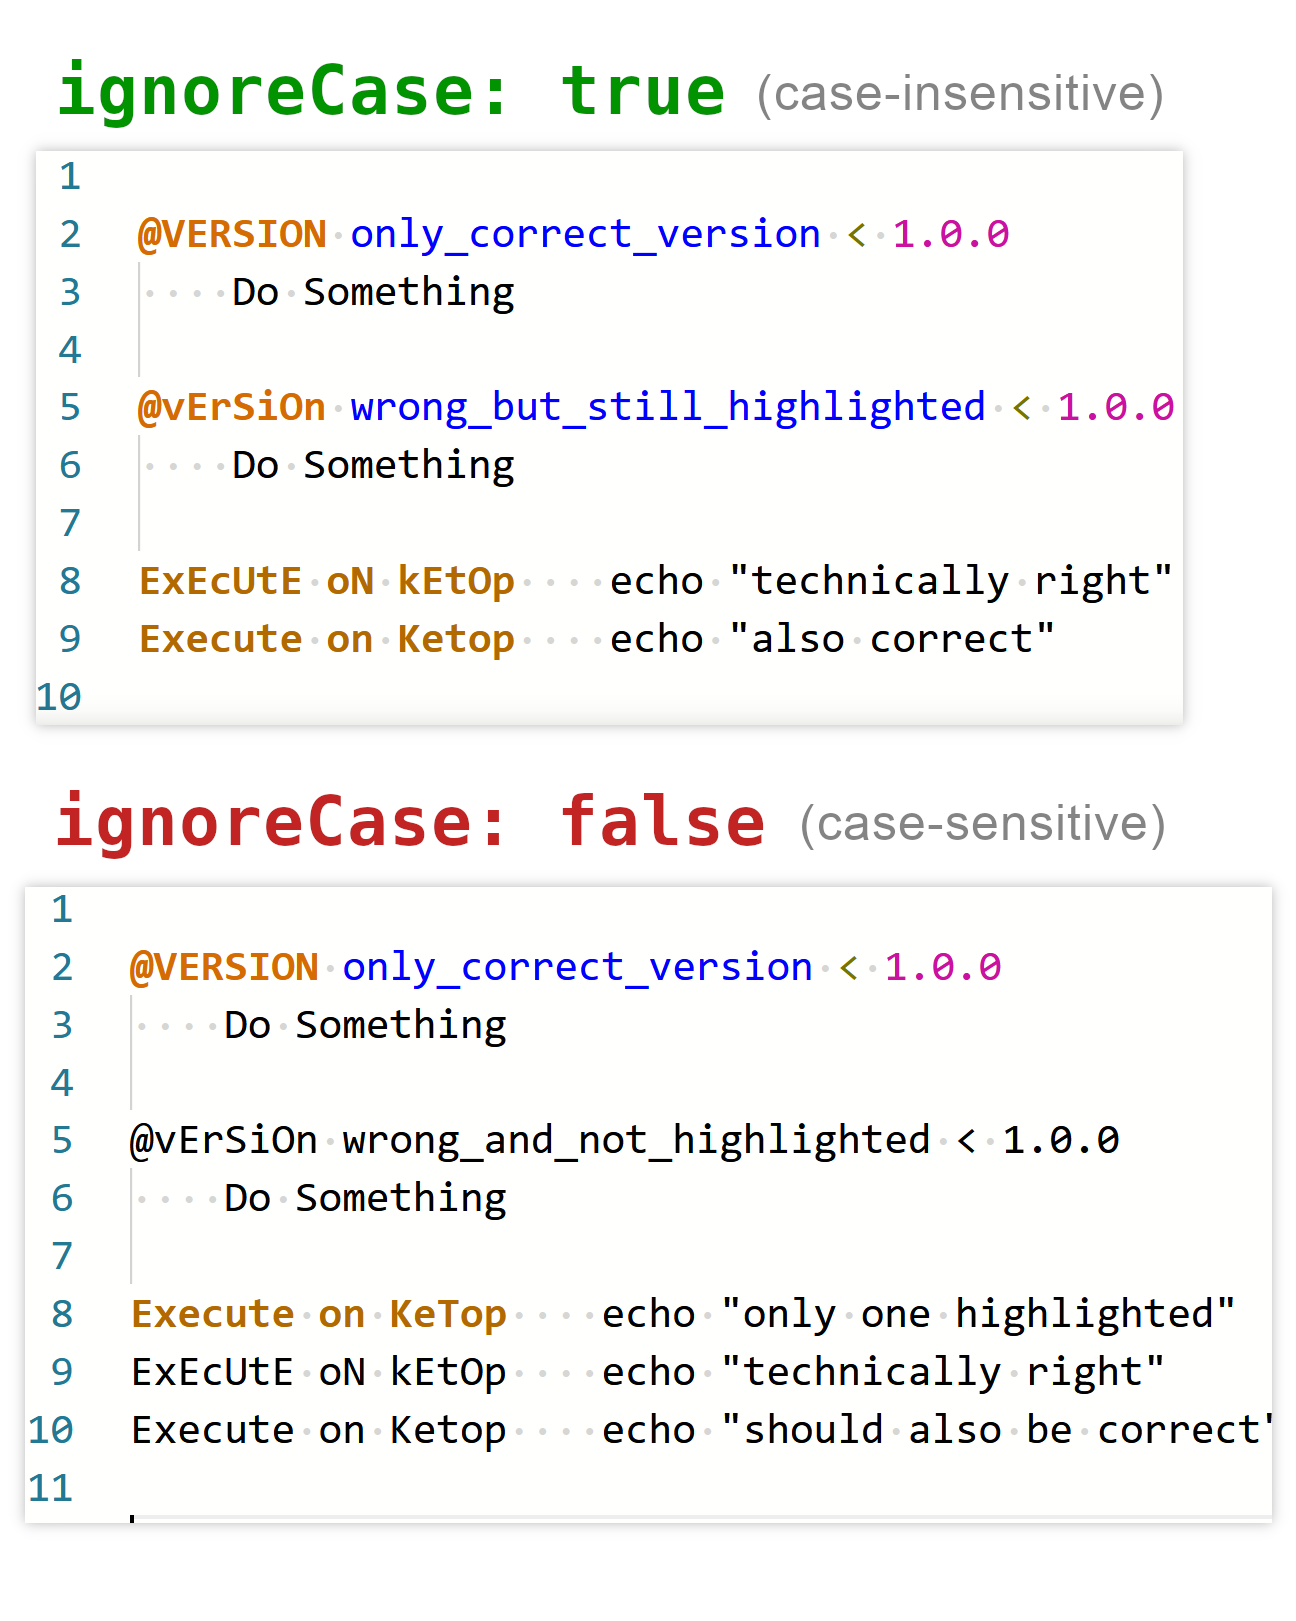
\includegraphics[width=0.8\linewidth]{pics/SyntaxHighlighting/case-sensitivity-issue.png}
    \caption{Case sensitivity issues in syntax highlighting}
    \label{fig:case-sensitivity-issue}
\end{figure}


The Monarch API only allows this setting for the entire language, because it is only possible through the global \texttt{ignoreCase} property defined in the \texttt{IMonarchLanguage} interface. A custom override for one tokenizer rule(\texttt{IMonarchLanguageRule}) or a single state is not possible. Therefore, the setting affects everything, the entire tokenizer. In the implemented editor configuration this global setting also affects the custom annotation rules, and as a result, if a developer types \texttt{@version} in lowercase, the frontend lexer still matches the rule and applies the corresponding syntax highlighting. But with the same script, the validation crashes when the backend EBNF parser takes the script. The reason is that the parser strictly needs the uppercase syntax \cite{MonacoMonarchTypes0341}.

This limitation leads to a small difference between the visual representation and the backend, but it is an unavoidable compromise. Disabling \texttt{ignoreCase} globally completely breaks the standard Robot Framework code highlighting, and that code is the vast majority of the file. That is why it is more important, that the base language simply has to function. This was the basis for the final architectural decision together with KEBA, even if it means the developer will only notice the error during transpilation and not while typing.



\chapter{Extensibility [F]}\label{chap:extensibility}
\setauthor{Filip Schauer}
% !TEX root = ../../thesis.tex

One of the most important requirements given by our project partner is that extending the project, by for example adding new keywords to the parser, should be as easy as possible. 

This chapter will go over the necessary steps required to define a new keyword or to write a seperate implementation of the parser. 

\section{Possibilities}

The parser is designed to make it particularly easy to define new keywords.

An option or a modifier may be defined to use, require, or optionally allow for an argument. Other keywords or parts of the parser may also be changed to react to the parser's current internal values, to the context of the scope that the keyword is used in, or to new or existing input data. 

If needed, it is possible to define keywords to allow for complex logic, for instance by adding an option that sets a variable to a chosen value and adding a modifier to compare it to a different variable.

What follows are a few of examples of keywords that we, for one reason or another, consider to be potentially useful within the context of the \gls{trp} project. 

\subsection{@LOADTEMPLATE}

In this example, \verb|@LOADTEMPLATE| is an option that takes a \textit{template name} as argument. \textit{Templates} could be passed as a dictionary, where each template name maps to a snippet of Robot Framework code that is commonly re-used across seperate test files. 

When this option is encountered, the parser could append the code snippet that belongs to the respective template to the current script or active bracket. 

This might allow for the reduction of code duplication, which could increase efficiency and maintainability. 

TODO: more examples

\section{Limitations}

Unfortunately, there are also some use cases where the core foundation that the parser is built on may not be sufficient. There are examples of features that, while they might be desirable for certain uses, are however thought to be particularly challenging to implement without rethinking the project from the ground up.

\subsection{Top-to-bottom processing}

Aside from the preprocessor, the parser traverses the file from the top to bottom. This means that, at any point of the file, it is currenty unaware of all keywords that are defined below, as the parser has not reached that point of the file yet.

\subsection{Naming}

The names of keywords must not include spaces and must be preceded by an \verb|@| character. Additionally, modifiers cannot have the same name as options, as they are differentiated by name only. 

\subsection{Multi-line}

Since arguments are defined to end when there a line break is encountered, it is not possible to have arguments that span across multiple lines.

Additionally, a keyword is only considered if, aside from inline whitespace, it is at the beginning of a line. 

\section{Adding a Keyword}

In general, there are three steps required to add a custom option or modifier to the parser:
\begin{enumerate}
    \item The keyword should be added to the \gls{ebnf}, which, from the root of the project, can be found in \verb|./TRP/config/script_assembler_ebnf.txt|.
    \item The keyword with its implementation should be added as a case to the parser. From the root of the project, the parser is found in \\\verb|./TRP/broker/managers/case/script_assembler|, and, within that folder, the core implementation of the keyword in \verb|option_modifier_format.py|. 
    \item The syntax highlighting for the keyword should be added. The definition for keywords used in syntax highlighting can be found in \\\verb|Angular/src/app/app.module.ts|. 
\end{enumerate}

TODO: example of exending with \verb|@LOADTEMPLATES|?

\section{Other purposes}

Since the parser treats Robot script lines as arbitrary pieces of text, and lines that do not start with an \verb|@| symbol generally pass through unchanged, the Script Assembler project may be used for purposes that transcend the domain of the \gls{trp} project that it was initially made for. 

In general, any project where simple, custom keywords may be needed to extend the capabilities of any text-based file might be a good use for Script Assembler. 

For instance, consider something that has nothing to do with \gls{trp}, like a product specification. Critical pieces of information that should not be given away to third parties could, for instance, be defined in a custom modifier named \verb|@SECRET|. Then, a boolean may be added as an input to the parser which decides whether the output should be a version of the specification that intended for internal use, or one that is fit to be sent to a third party. 


\chapter{Database [X]}\label{chap:database}
\setauthor{Axel Csomány}
Besides the extension of the Script Assembler's capabilities and the creation of a new EBNF language that makes the software more extendable, another main focus of the project is the creation of a mockup of the TestRail database. This mockup is not only made for testing purposes, but allows the user to work independently of the TestRail instance. The mockup is designed to be as close to the real TestRail database as possible, allowing a seamless switch between the two instances. This means that all functionalities that are available in the real TestRail database are also available in the new mockup.

This section aims to give an overview of the different types of databases, the structure and functionalities of the TestRail database specifically, the resulting design and implementation of the mockup database, and the way the database switch is finally implemented.

\section{Types of Databases}

Depending on the requirements of a given project, different types of databases are suitable for different use cases. It is important to analyze what qualities are needed and which qualities are negligible to find the best fitting solution. 

The most important qualities of a database type can be expressed in the following categories:

\begin{itemize}
    \item \textbf{Data Model:} \\
    The data model of a certain database type describes how the data is structured and stored. This can be in the form of tables, documents, graphs or other structures. The data model has a notable impact on aspects like performance and scalability.

    \item \textbf{Storage Architecture:} \\
    The storage architecture of a database type not only describes how the data is stored, but also how it may be accessed, managed and distributed. This can be in the form of a single server, a cluster of servers or even a distributed network of servers across the globe.

    \item \textbf{Query Model:} \\
    The query model of a database type describes the means of accessing the data. This can occur in the form of a specifically designed query language, an API or other methods. This has an undeniable impact on the ease of use of the database and how the user writes and optimizes queries.
\end{itemize}

Based on these qualities, various databases types have been developed, each with their own unique advantages and disadvantages. Some of the most common types of databases include but are not limited to relational databases, object-oriented databases and NoSQL databases, which can be further categorized by the data model they use, such as document stores, key-value stores, column-family stores and graph databases \cite{DigitalOceanDatabaseTypes}.

\section{Relational Databases}

For the purpose of this project, we will take a closer look at relational databases, as this is the type of database that TestRail uses. 

\subsection{Structure of Relational Databases}

Relational databases are based on the relational model, which organizes its data into tables, consisting of rows and columns. Each table represents a specific entity and each row in the table represents an instance of that entity. The columns in the table represent the attributes of the entity. 

Relationships between these entities can be established through the use of keys. A primary key is a unique identifier for each instance of an entity, while a foreign key is a reference to the primary key of another entity. Meaningful relationships between entities can be built with the usage of these keys, allowing complex queries to be executed across multiple linked entities \cite{WikipediaRelationalDatabase}.

Grouping in queries allows for the aggregation of data based on specific attributes, while joins allow for the combination of data from multiple tables based on the established relationships.

\begin{figure}[ht]
    \centering
    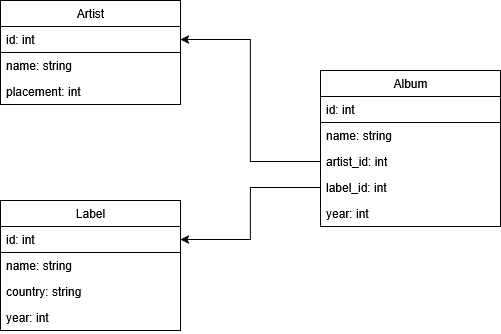
\includegraphics[width=0.8\textwidth]{pics/simple-erd.png}
    \caption{Simple Diagram showcasing the relationship between three entities in a relational database.}
    \label{fig:erd}
\end{figure}

In figure \ref{fig:erd}, we can see a simplified example of a relational database structure. The three entities "Artist", "Label" and "Album" are represented as tables, with their respective attributes as columns. The relationships between the entities are established through the usage of primary and foreign keys, allowing for queries to be executed across multiple linked entities. For example, we can query for all albums by a specific artist or a specific label.

\subsection{ACID}

ACID is an acronym that stands for the four key properties of a safe database transaction:

\begin{itemize}
    \item \textbf{Atomicity:} \\ 
    Atomicity ensures that a transaction, which is often a sequence of multiple operations, is treated as a single unit. This means that either all operations within a given transaction are executed successfully, or none of them are. If any operation of the transaction fails due to an error, a power outage or any other issue, the entire transaction is rolled back to its previous state before the transaction began. This guarantees that the database remains consistent and prevents data corruption or loss that could occur if only part of the transaction were to be executed.
    
    \item \textbf{Consistency:} \\
    Consistency ensures that the database can only be brought from one valid consistent state to another, while following all defined rules, constraints and triggers. Invalid transactions that violate any of the defined rules are rolled back accordingly, ensuring that the database remains consistent.
    
    \item \textbf{Isolation:} \\
    Isolation ensures that concurrent transactions have no impact on each other. This means that the effects of a transaction in progress are not visible to other transactions until it completes successfully. This prevents a number of issues that would otherwise arise from concurrent transactions, like dirty reads, where one transaction reads data that has been modified by another transaction but not yet fully committed, potentially leading to incorrect results.
    
    \item \textbf{Durability:} \\ 
    Durability ensures that once a transaction has been successfully completed and committed, the state of the database persists even in the case of a crash, power failure or any other issue. 
\end{itemize}

Databases that adhere to these properties are considered to be reliable and safe for use in critical environments, as they guarantee that the data not only remains consistent, but also that it is not lost or corrupted due to unforseen events \cite{WikipediaACID}.

\subsection{Advantages and Disadvantages of Relational Databases}

One of the main strengths of relational databases is their ability to handle long and complex queries across multiple linked entities with the usage of foreign keys and joins. The consistency and integrity of the data is guaranteed by the ACID properties. On top of that, relational databases are some of the most widely used and well-known types of databases, which means that there are a lot of resources and a large community available for support and development. 

However, relational databases can struggle with scalability and performance when dealing with large volumes of data or high traffic. The fixed schema of relational databases can also be a disadvantage, as it can make it difficult to adapt to changing requirements or to handle unstructured data. Additionally, the execution of complex queries can lead to performance issues on larger datasets.

\section{The TestRail Database}

TestRail is a web-based test management tool that provides a wide range of features for managing and organizing test cases, test runs and test results. The relational database in the background of TestRail is used to store all of the data related to these features. The user can interact with the database directly by using the TestRail API, although the database itself is not directly accessible to the user. 

Thus, for the creation of the mockup database, the structure and functionalities of the TestRail database have to be studied and analyzed based on the API documentation and the structure of its response data. While the mockup database doesn't have to be an exact replica of the TestRail database, the functionalities used by the Script Assembler need to deliver responses with identical structure to ensure the switch between databases can occur without any issues.

In order to achieve this, the most important entities and their relationships have to be identified.

\subsection{Test Cases}

Test cases can be seen as the most fundamental entity in the TestRail system, as they represent the individual tests that are to be executed. Test cases have a number of attributes, such as a title, description, type and the test steps that need to be executed. Test cases are furthermore linked to test suites and sections. 

\subsection{Projects, Suites and Sections}

Projects are the highest level of organization in TestRail, representing a specific testing effort or initiative. Each project can contain multiple test suites, which are collections of test cases. The test cases of Suites can further be organized into sections, allowing for more specific grouping and categorization. These relationships are an essential part of the database structure that needs to be replicated.

\subsection{Test Runs}

A test run represents a specific execution of test cases. Test runs are linked to test cases and contain information about the execution, such as the status of each case, the tester who executed the run and any relevant comments or other metadata. Test runs make the tracking and management of test executions possible. Importantly, a test run can only be created for test cases that are contained in one singular test suite.

\subsection{Test Plans}

Test plans are used to organize and manage test runs. TestRail allows the user to group multiple test runs into a test plan, which alleviates the need to manage each run individually.

\subsection{Test Results}

Test results represent the outcome of a test case within a test run. Test results mainly consist of a status, which can contain, but is not limited to:

\begin{itemize}
    \item \textbf{Passed} \\
    A test case is marked as passed when it has been successfully executed and all results are as expected.

    \item \textbf{Failed} \\
    A test case is marked as failed when it has been executed but the results are not as expected, meaning that the tested functionality does not work as intended.

    \item \textbf{Untested} \\
    A test case that hasn't been assigned a status yet is marked as untested.

    \item \textbf{Retest} \\
    A test case is marked as retest when it has failed previously, but has been fixed and is now ready to be tested again.

    \item \textbf{Blocked} \\
    A test case is marked as blocked when it cannot be executed due to an error that is not related to the functionality being tested.
\end{itemize}

\subsection{Users}

Users represent the individuals who interact with the TestRail system. Users can have different roles and permissions within the system. They can be assigned to test runs, test plans or other entities as creators. With the user entity it is possible to track who is responsible for which run and plan.

\section{PostgreSQL}

For the implementation of the mockup database, PostgreSQL was chosen as the database management system, as it is an open-source database that is not only widely used but also well-known for its reliability and performance. 

PostgreSQL is not only a database management system that the team is familiar with, but it also provides all the necessary features and capabilites needed for the implementation of this part of the project. It supports the relational data model, which is needed for replacing the TestRail database, and it guarantees the reliability and consistency of its data with the ACID properties.

\subsection{pgAdmin}

The open-source management tool "pgAdmin" is used for the administration of the PostgreSQL database, as it provides an easily navigable user interface for management, query execution and other administrative tasks.

\begin{figure}[ht]
    \centering
    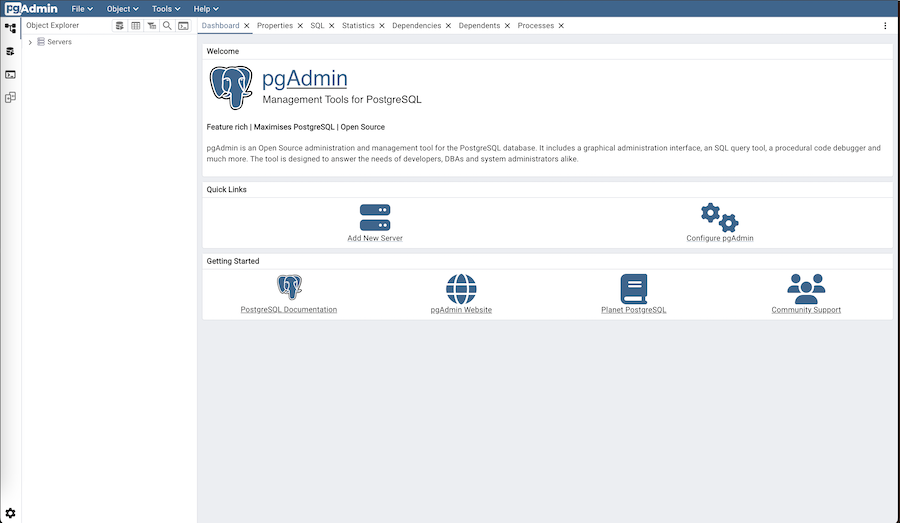
\includegraphics[width=0.95\textwidth]{pics/pgadmin-interface.png}
    \caption{Screenshot of the pgAdmin interface \cite{pgAdminInterface}.}
    \label{fig:pgadmin-interface}
\end{figure}

The current version of pgAdmin, which is pgAdmin 4, provides a wide range of features for managing and administering PostgreSQL databases, some of which include but are not limited to the following: \cite{pgAdminInterface}.

\begin{itemize}
    \item \textbf{SQL query tool:} \\
    Inside pgAdmin, there is a built-in SQL editor that allows users to write and execute SQL queries directly against the database. This tool provides syntax highlighting, further aiding the user in writing correct queries.

    \item \textbf{Direct data editing:} \\
    The tables in a database can be directly edited through the interface, allowing for quick and easy modifications of single points of data without the need to write and execute SQL queries. Caution should be taken when using this feature however, as the quick and easy nature of this feature can lead to unintended consequences.

    \item \textbf{Management of multiple databases:} \\
    The pgAdmin interface allows the management of multiple databases within the same interface, allowing for intuitive switching between independent databases. 
\end{itemize}

\section{First Approaches}

Early into the development of the database, two main approaches were considered for how the database should interact with the backend of the main system. 

One approach was to create an API that would allow the main system to interact with the database through API calls. This would have resulted in a clear separation between the database and the main system.

The other approach was to work in the preexisting backend to connect to the database directly. This approach was ultimately chosen, as it not only makes the switch between the two databases simpler, but also integrates the functionality of the new database directly into the main system. This approach was further endorsed by the supervisor of the project, as it helps the system to eventually transition away from the TestRail database and towards the new mockup database, which allows for more independence and expandability in the future.

The python library "psycopg" is used for the connection between the main system and the PostgreSQL database. This library provides a simple and efficient way to connect to the PostgreSQL database and execute various commands and queries. It also provides support for connection pooling, which can help to improve the performance of the database interactions.

\section{Database Connections in the System}

The following section aims to give a brief look into the structure and functionalities of not only the existing TestRail database connection, but also the new PostgreSQL mockup database. The goal is to show how the new database is designed to replicate the implementations of the TestRail connection, while also highlighting clear differences on a technical level.

\subsection{Existing TestRail Functionality}

The existing funtionalities concerning the TestRail connection is contained within the TRSession class, which is responsible for all interactions with the database. This class contains functions for retrieving and creating test cases, runs, plans and results, as well as other relevant data. 

The communication with the TestRail database is achieved through the usage of the TestRail API, which provides all necessary reading and writing functionalities.

\begin{lstlisting}[caption={Code snippet of the get\_case\_title function within the TRSession class.}, label={lst:tr-function}]

    def get_case_title(self, case_id: int, safe_name: bool = False) -> str | None:
        response = self.do_request(f"get_case/{case_id}", TRConst.REQUEST_TYPE_GET)
        if not response:
            return None
        if len(response) <= 0:
            self.log.warning(f"could not find a result for test case: {case_id}")
            return None
        if not safe_name:
            return response['title']
        return response['title'].replace(":", "")

\end{lstlisting}

In listing \ref{lst:tr-function}, one of the functions of the TRSession class can be seen. This function is responsible for retrieving the title of a test case based on its ID. Using the ID of the wanted test case, a GET request is sent to the TestRail API, which then returns the relevant data. The function then processes the response data and returns the title. 

All functions of the TRSession class follow a similar structure, with the type of interaction with the API being the main difference. For example, functions that create new entities in the database use POST requests and send the relevant data in the body of the request.

\subsection{DBSession}

The DBSession class is designed to replicate all used functionalities of the exisitng TRSession class, while replacing the communication with the TestRail API with a direct connection to the PostgreSQL database, using the "psycopg" python library. It is strictly necessary that the functions of the DBSession have the same name, parameters and return values as the functions of the TRSession class, in order to avoid major conflicts when switching between the two database connections.

\begin{lstlisting}[caption={Code snippet of the get\_case\_title function within the DBSession class.}, label={lst:db-function}]

    def get_case_title(self, case_id: int, safe_name: bool = False) -> str | None:

        if case_id == None:
            print("Did not get a case_id")
            return None
        
        if case_id < 0:
            print(f"Invalid value for case_id: {case_id}")
            return None
        
        self.cursor.execute("SELECT title FROM test_cases WHERE id = %s", (case_id,))

        result = self.cursor.fetchone()

        if result != None:
            return str(result[0])
        
        return None

\end{lstlisting}

In listing \ref{lst:db-function}, the same function as in listing \ref{lst:tr-function} can be seen, but this time within the DBSession class. Thus, while the parameters and return value of the function are identical to the one in the TRSession class, the implementation is different.

Instead of interacting with an API, this function uses a connection to the PostgreSQL database to execute a SQL query that retrieves the title of the specified test case. 

\section{Integration of the DBSession Class}

Since the DBSession class replicates all essential functions of the TRSession class, the switch between database usages can be achieved easily.

Any occurrence of the TRSession class within the backend of the system is now denoted as a TRSession or DBSession, using a pipe symbol. This means that at system startup, the appropriate session class has to be identified and initialized accordingly. 

\begin{lstlisting}[caption={Code snippet showcasing a function that takes a parameter that can be either a TRSession or a DBSession.}, label={lst:tr-or-db}]

    def fetch_cases(self, testrail: TRSession | DBSession):
        # Function implementation

\end{lstlisting}

This way, the TRSession functionalities remain unaltered, while the possibility of using the DBSession is a new feature that can be easily switched on or off.

\subsection{Switching Between Databases}

The switch between the two databases is implemented in a way that allows the user to easily and definitively choose which database should be used at the execution of the python script. This is achieved by using a command line argument that can be passed when executing the script. The argument is then processed and the appropriate database instance is initialized based on if the argument is present or not. 

\begin{verbatim}
    python ./broker.py
\end{verbatim}

Here, the standard TestRail database is used, as no argument is passed to the script.

\begin{verbatim}
    python ./broker.py -db
    # OR
    python ./broker.py --database
\end{verbatim}

Here, the PostgreSQL mockup database is used, as the argument is passed to the script. The argument can either be a short version, or a long version, as both are processed in the same way and lead to the same result.

\section{The PostgreSQL Database}

Since the structure of the TestRail database is not publicly available, the structure of the PostgreSQL mockup database is based on the structure of the response data the TestRail API provides. All entities contain their respective attributes, as well as keys that establish the relationships between the different entities.

It is important to note that the relationships between entities are not made with the usage of foreign keys, as the logic for the relationships is implemented in the backend of the system, and the database is only used for storing data. While this is not the most efficient way to implement the relationships between entities, as a mockup database, it is sufficient for the purpose of this project. Despite that, in section \ref{sec:potential-future-steps}, potential future steps are discussed, one of which is the implementation of proper relationships between entities with the usage of foreign keys.

The database contains tables for all the entities of the TestRail system, that are relevant for the functionalities of the Script Assembler. All entities are listed below, along with their respective attributes.

Every entity contains an \textit{id} attribute, signifying the unique identifies for each instance of the entity, with the datatype of \textit{serial}, which means that the integer value of the attribute is automatically incremented with each new instance of the entity. Since this attribute is present in all entities, it will not be listed for each entity separately.

\subsection{Case Types}

Case Types are used to categorize the test cases based on their type, such as functional, performance or security test cases. This is mainly used to group test cases together and strictly serve the organizational purposes of the system.

This table has the following attributes:
\begin{itemize}
    \item \textbf{is_default:} \\
    This attribute is a boolean value that is set to true for one specific case type, which is assigned as the default case type. All other case types have this attribute set to false.

    \item \textbf{case_name:} \\
    This attribute is a string value that contains the name of the case type.
\end{itemize}

\subsection{Groups}

Groups are used to categorize users based on their roles, permissions or tasks. Similarily to case types, groups are mainly used for organizational purposes.

This table has the following attributes:
\begin{itemize}
    \item \textbf{name:} \\
    This attribute is a string value that contains the name of the group.

    \item \textbf{user_ids:} \\
    This attribute is an array of integers that contains the IDs of all users assigned to the specific group.
\end{itemize}

\subsection{Priorities}

Priorities are used to order test cases in the system. Test cases with a higher value of priority are considered more important and are therefore executed before others with a lower value of priority. This also influences the ordering of test cases in the user interface, as well as the order they are assembled in the final script.

This table has the following attributes:
\begin{itemize}
    \item \textbf{is_default:} \\
    This attribute is a boolean value that is set to true for one specific priority, which is assigned as the default priority. All other priorities have this attribute set to false.

    \item \textbf{prio_name:} \\
    This attribute is a string value that contains the name of the priority.

    \item \textbf{priority:} \\
    This attribute is an integer value that contains the priority level, with higher values corresponding to a higher priority.

    \item \textbf{short_name:} \\
    This attribute is a string value that contains a short name alternative for the priority.
\end{itemize}

\subsection{Projects}

Projects are the uppermost level of organization in the system. They contain other entities such as test suites and by extension sections and test cases. Projects represent a specific testing effort or testing environment for an entire system.

This table has the following attributes:
\begin{itemize}
    \item \textbf{announcement:} \\
    This attribute is a string value that contains the announcement message for the project, which provides more information about the project and its purpose.

    \item \textbf{default_role_id:} \\
    This attribute is an integer value pointing to the ID of the role that is assigned as the default role for the project. This role is automatically assigned to all users that are added to the project, unless they are assigned a different role.

    \item \textbf{default_role:} \\
    This attribute is a string value that contains the name of the default role.

    \item \textbf{is_completed:} \\
    This attribute is a boolean value that indicates whether the project has been completed or not.

    \item \textbf{project_name:} \\
    This attribute is a string value that contains the name of the project.

    \item \textbf{show_announcement:} \\
    This attribute is a boolean value that indicates whether the announcement message of the project should be shown to users or not.

    \item \textbf{url:} \\
    This attribute is a string value that contains the URL of the project.

    \item \textbf{users:} \\
    This attribute is an array of integers that contains the IDs of all users assigned to the project.

    \item \textbf{completed_on:} \\
    This attribute is an integer value that contains the UNIX timestamp of when the project was completed.
\end{itemize}

\subsection{Test Suites}

Test Suites are collections of test cases that are grouped together based on their purpose or functionality.

This table has the following attributes:
\begin{itemize}
    \item \textbf{description:} \\
    This attribute is a string value that contains the description of the specific test suite.

    \item \textbf{name:} \\
    This attribute is a string value that contains the name of the test suite.

    \item \textbf{project_id:} \\
    This attribute is an integer value that contains the ID of the project that the test suite is assigned to.

    \item \textbf{url:} \\
    This attribute is a string value that contains the URL of the test suite.
\end{itemize}

\subsection{Sections}

Sections further divide and organize the test cases within a test suite.

This table has the following attributes:
\begin{itemize}
    \item \textbf{depth:} \\
    The depth attribute is an integer value that indicates the level of the section within the hierarchy of sections. The lower the value, the higher the section is in the hierarchy.

    \item \textbf{description:} \\
    This attribute is a string value that contains the description of the specific section.

    \item \textbf{display_name:} \\
    This attribute is a string value that contains a name of the section as it should be displayed in the user interface.

    \item \textbf{name:} \\
    This attribute is a string value that contains the name of the section.

    \item \textbf{parent_id:} \\
    Sections can be nested within other sections, which can be achieved by assigning a section as the parent of another. This attribute is an integer value that contains the ID of the parent section, if there is one. If this section is in the uppermost level of the hierarchy, it does not have a parent and therefore this attribute is set to null.

    \item \textbf{suite_id:} \\
    This attribute is an integer value that contains the ID of the test suite that the section is assigned to.
\end{itemize}

\subsection{Test Cases}

This table has the following attributes:
\begin{itemize}
    \item \textbf{} \\
\end{itemize}

\subsection{Test Results}

This table has the following attributes:
\begin{itemize}
    \item \textbf{} \\
\end{itemize}

\subsection{Test Runs}

This table has the following attributes:
\begin{itemize}
    \item \textbf{} \\
\end{itemize}

\subsection{Tests}

This table has the following attributes:
\begin{itemize}
    \item \textbf{} \\
\end{itemize}

\subsection{Users}

This table has the following attributes:
\begin{itemize}
    \item \textbf{} \\
\end{itemize}

\section{Potential Future Steps} \label{sec:potential-future-steps}

\subsection{Easier Creation of Test Cases}

TestRail provides a functionality for the creation of test cases through the API, as well as through their user interface. This makes the creation of new test cases in the database an easy task, especially with the user interface, as the user can efficiently create new test cases and other entities without having to worry about the structure of the database itself.

Currently, the creation of test cases in the PostgreSQL database is done manually by either executing SQL queries manually or by making use of the pgAdmin user interface. This is not only time-consuming, but also prone to errors, as the user has to ensure that all necessary attributes of the test case are filled in correctly and that the relationships between entities are established properly.

A potential future step to fix this issue would be to create a user interface that allows for the easier creation of test cases and other entities in the database. This system could either be a separate application that interacts with the database on its own, or it could be integrated into the existing system. 

\subsection{Information Security}

For convenience and ease of use, the users of the PostgreSQL database currently have their credentials stored in plain text within their respective columns in the database. While this is not an issue for the mockup database, as it is only used for testing purposes, if the PostgreSQL database approach is to be used in the future as a replacement for the TestRail database, it would be necessary to implement a system for encrypting or hashing the credentials of all users, in order to ensure the security of the database and the data it contains. 

This could be achieved by using a hashing algorithm to hash the passwords before storing them in the database, and then comparing the hashed password with the stored hash when a user attempts to log in. This would ensure that actual passwords cannot be retrieved from the database, even if the database is compromised.

Hasing is an irreversible process, meaning that once a password is hashed, it cannot be converted back to its plain text form. Encryption, on the other hand, is a reversible process, so it would be possible to retrieve the original password from the encrypted form if the key is known. While hashing is more secure for storing passwords, both methods are viable options for ensuring the security of credentials in the database.

\subsection{Implementation of Proper Relationships}

The relationships between entities in the PostgreSQL database are not implemented with the usage of foreign keys, but rather with the usage of keys that are processed in the backend of the system. The logic for the relationships is implemented in the backend, which means that the database is only used for strictly storing data. 

This is not the most efficient way to implement relationships, as it can lead to issues with data integrity, as well as performance issues when executing queries that involve multiple linked tables.

The logical next step to improve the implementation of the database would be to implement proper relationships between entities with the correct usage of foreign keys. 

\newpage
\pagenumbering{Roman}
\setcounter{page}{\value{RPages}}
%\setlength{\glsdescwidth}{0.8\linewidth}
\glsnogroupskiptrue
\glsaddall
\IfStrEq{\thesislang}{de}
{
	\printglossary[title=Glossar,toctitle=Glossar] %,style=long]
}
{
	\printglossary[title=Glossary,toctitle=Glossary] %,style=long]
}
\IfStrEq{\thesislang}{en}{
    \renewcommand{\refname}{References}
    \renewcommand{\bibname}{References}
}

\IfStrEq{\thesislang}{de}
{
	\bibliographystyle{ieeetrande}
}
{
	\bibliographystyle{IEEEtran}
}
\nocite{*}
\bibliography{bib}

\listoffigures
%\listoftables
\lstlistoflistings
\appendix
\addchap{Appendix}
% !TEX root = ../thesis.tex

\section*{Project Timeline}

\section*{Filip Schauer's Takeaways}

\section*{Axel Csomány's Takeaways}

\section*{Adam Höllerl's Takeaways}
\end{document}
